\documentclass[12pt,titlepage]{article}
\usepackage[margin=1in]{geometry} 
\usepackage{amsmath,amsthm,amssymb,graphicx,mathtools,tikz,hyperref}
\usepackage{pgfplots}
\usepackage{xcolor}
\newcommand{\redp}[1]{\textcolor{red}{#1}}
\newcommand{\bluep}[1]{\textcolor{blue}{#1}}
\newcommand{\tealp}[1]{\textcolor{teal}{#1}}
\usetikzlibrary{patterns,hobby}
\numberwithin{equation}{section}
\usepackage{wrapfig}
\usepackage{indentfirst}
\usepackage{ragged2e}
\RaggedRightParindent = 24 pt
\setlength{\parskip}{0.8em}
\renewcommand{\baselinestretch}{1.5}
\usepackage[noline]{algorithm2e}
\SetAlFnt{\footnotesize}
\usepackage{graphicx}
\usepackage{titling}
\renewcommand\maketitlehooka{\null\mbox{}\vfill}
\renewcommand\maketitlehookd{\vfill\null}
\usepackage{tocloft}
\renewcommand\cftsecafterpnum{\vskip6pt}
\usepackage{makeidx}
\makeindex

\title{Notes on Phase Transition and RG}
\author{Sizhe Liu\\Department of Mechanical Science and Engineering
\\University of Illinois at Urbana-Champaign}
\date{Version 1.0}

\begin{document}

\maketitle

\section{Introduction}
\subsection{Scaling and dimensional analysis}
The phenomena of phase transitions all exhibit \textbf{scaling}. This just means that two measurable quantities depend on each other in a \emph{power-law} fashion. For example, we can write the formula for the phase speed \textit{c} of waves on shallow water of depth $h$ as:
\begin{equation}
    c^2=gh
\end{equation}
where the surface tension and viscous effect are neglected. The scaling law in this case is $c\propto\sqrt{h}$.

Often, scaling laws can easily be deduced from \textbf{dimensional analysis}. In the water wave case, we have $[g]=LT^{-2}$, $[h]=[\lambda]=L$ and the unit of density is $[\rho]=ML^{-3}$. Thus
\begin{equation}
    c=(gh)^{1/2}f(\frac{h}{\lambda})
\end{equation}
where $f$ is a function that cannot be determined by dimensional analysis. In the limit $h/\lambda\rightarrow 0$,
\begin{equation}
    c \sim (gh)^{1/2}f(0)\propto\sqrt{h},
\end{equation}
recovering the scaling law, without requiring any detailed knowledge about fluid dynamics.

However, this happy derivation is an \emph{illusion--we assumed that the limiting case was regular}. In fact, \textbf{the cases where the regularity assumption breaks down constitute the phase transition phenomena.}

\subsubsection{Magnetic critical point}
At high temperature and zero external field, the system is in the \textbf{paramagnetic\index{paramagnetic} }phase: following the time evolution of any spin would reveal that it points in all directions with equal frequency.

Below a \textbf{critical temperature}, $T_c$, however, the spins tend to align along a particular direction in space, even in the absence of an external field. In this case, there is a net \textbf{magnetisation\index{magnetisation}}, $M(T)$, and the system is in the \textbf{ferromagnetic\index{ferromagnetic}} phase. The onset of this behavior is a \textbf{continuous phase transition}: the magnetisation rises \textit{continuously} from zero as the temperature is reduced below $T_c$. A quantity which varies in this way is referred to as an \textbf{\index{order parameter}}.

\subsection{Some important questions}
First, we examine the Ehrenfest's classification of phase transition. Ehrenfest proposed that phase transtions could be classfied as "$n^{th}$ order" if any $n^{th}$ derivative of the free energy with respect to any of its arguments yields a discontinuity at the phase transition. The phenomena which are called as \textbf{critical phenomena} usually occur at \textbf{continuous order phase transition\index{continuous order phase transition}}. Ehrenfest's classification fails because at the time that it was formulated, it was not known that thermodynamic quantities such as the specific heat actually \emph{diverge at continuous transitions}, rather than exhibiting a simple \textbf{discontinuity} as Ehrenfest implies.

\textbf{Question 1: \emph{Why do phase transitions occur at all?}}

In statistical mechanics, thermodynamics arises from the free energy, $F$, and its derivatives, given by Gibb's formula:
\begin{equation}
    e^{F/k_BT} = Tr e^{-H/k_BT}
\end{equation}
where $Tr$ denotes a sum over all degrees of freedom mentioned in $H$. Since the Hamiltonian will usually be a non-singular function of the degree of freedom, the \emph{patition function is nothing more than a sum of exponentials of analytic function of the parameters in the Hamiltonian}. How, then, can such a sum give rise to \emph{non-analytic} behavior? Is it even clear \emph{a priori} that a single partition function can describe multiple phases?

\textbf{Question 2: \emph{Why does universality occur, and what are the factors that determine which set of phenomena have the same critical exponents?}}

Phenomena with the same set of critical exponents are said to form a \textbf{universality class\index{universality! class}}. The usefulness of the concept lies in the fact that, in general, members of a universality class have three things in common:\textbf{the symmetry group of the Hamiltonian (not the lattice), the dimensionality, and whether or not the forces are short-ranged.}

\subsection{Solution to Exercises}
\subsubsection{Prove Pythagoras' theorem using dimensional analysis}
\begin{wrapfigure}{r}{5cm}
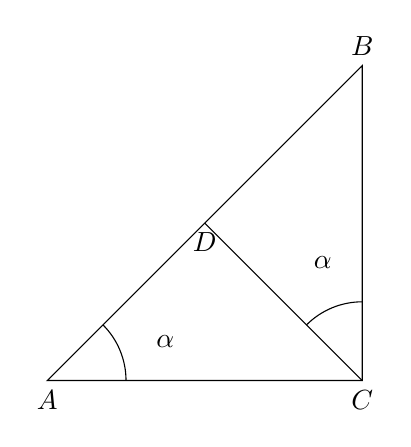
\begin{tikzpicture}
\draw (0,0) node[anchor=north]{$A$}
  -- (4,0) node[anchor=north]{$C$}
  -- (4,4) node[anchor=south]{$B$}
  -- cycle;
\draw (4,0)--(2,2) node[anchor=north]{$D$};
\draw (1, 0) arc (0:45:1cm);
\draw (4, 1) arc (90:135:1cm);
\draw (1.5, 0.5) node{$\alpha$};
\draw (3.5, 1.5) node{$\alpha$};
\end{tikzpicture}
\end{wrapfigure}
From the figure, we know the area of $\Delta ABC$ is $A_{ABC}=f(d_{AB},\alpha)$. Similarly, we have $A_{ADC}=f(d_{AC},\alpha)$, $A_{BDC}=f(d_{BC},\alpha)$. According to dimensional analysis, we can write these relations as:
\begin{equation}
\begin{split}
    A_{ABC}=d^2_{AB}g(\alpha)\\
    A_{ADC}=d^2_{AC}g(\alpha)\\
    A_{BDC}=d^2_{BC}g(\alpha)
\end{split}
\end{equation}
Because $A_{ABC}=A_{ADC}+A_{BDC}$, we arrive at
\begin{equation}
    d^2_{AB}=d^2_{AC}+d^2_{BC}
\end{equation}

\subsubsection{Scaling law of radius R of blast versus time t}
The units of related quantities are:
\begin{equation}
\begin{split}
    [E]=ML^2T^{-2}\\
    [\rho] = ML^{-3}\\
    [E/\rho]=L^5T^{-2}
\end{split}
\end{equation}
Because $E/\rho$ is a constant, we have 
\begin{equation}
    \begin{split}
        f(R,t)=\frac{E}{\rho}\sim R^5t^{-2}\\
        \Rightarrow R\propto t^{2/5}
    \end{split}
\end{equation}

\section{How Phase Transitions Occur in Principle}
\subsection{Review of statistical mechanics}
The goal of statistical mechanics is to compute the partition function $Z$. We specify the system of interest as some sample region $\Omega$, in which is defined the Hamiltonian $H_{\Omega}$. The volume of the region is $V(\Omega)$ and the surface area is $S(\Omega)$. Often it will be convenient to think of our system as having some characteristic linear dimension $L$, so that $V(\Omega)\propto L^d$ and $S(\Omega)\propto L^{d-1}$, where $d$ is the dimensionality of the system.

Usually, there will be \textbf{boundary conditions} specified on the boundary of $\Omega$. Often these will be periodic or hard wall. The system may exist as a continuum (\emph{e.g., fluid}) or a lattice; for now, $V(\Omega)$ is finite. We then write the Hamiltonian for the system as:
\begin{equation}
    -\frac{H_{\Omega}}{k_BT}=\sum_nK_n\Theta_n
\end{equation}
where $K_n$ are the \textbf{coupling constants}\index{coupling constants} and the $\Theta_n$ are combinations of the dynamical degree of freedom (DOI), which are summed over in the partition function. We shall sometimes refer to the $\Theta_n$ as \textbf{local operator}\index{local operator}. In an example of a magnet, the DOI are the spins on the lattice sites $\boldsymbol{S}_i$, where $1\leq i \leq N(\Omega)$. Thus, $\Theta_1=\sum_i\boldsymbol{S}_i$, $\Theta_2=\sum_{ij}\boldsymbol{S}_i\cdot\boldsymbol{S}_j$, etc. In this context, 
\begin{equation}
    Tr\equiv\sum_{S_1}\sum_{S_2}...\sum_{S_N}
\end{equation}
where each sum is over all possible values that each spin can take. The partition function itself is given by
\begin{equation}
    Z[{K_n}]\equiv Tr e^{-\beta H_{\Omega}}
\end{equation}
After carrying out the trace, $Z$ depends on all of the $K_n$. We shall sometimes indicate this dependence on the entire set of coupling constants as:$[K]\equiv[{K_n}]$.

The \textbf{free energy}\index{free energy} is defined by
\begin{equation}
    F_{\Omega}[{K_n}] = -k_BT log Z_{\Omega}
\end{equation}
and information on the thermodynamics of the system $\Omega$ is contained in the derivatives of free energy.

\subsection{The thermodynamic limit}
The free energy is extensive for a large system:$F_{\Omega}\propto V(\Omega)$. Thus, we expect that for a finite system, we can write
\begin{equation}
    F_{\Omega} = V(\Omega)f_b + S(\Omega)f_s+O(L^(d-2)),
\end{equation}
where $f_b$ is the \textbf{bulk free energy}\index{bulk free energy} per unit volume or \textbf{bulk free energy density} and $f_s$ is the \textbf{surface free energy}\index{surface free energy} per unit area. A precise definition of these quantities are given as follows:
\begin{equation}
\begin{split}
    f_b[K]\equiv\lim_{V\rightarrow\infty}\frac{F_{\Omega}[K]}{V(\Omega)},\textit{ or}\\
    f_b[K]\equiv\lim_{N\rightarrow\infty}\frac{F_{\Omega}[K]}{N(\Omega)}.
\end{split}
\end{equation}
To describe surface or finite size behavior, we need to compute the surface free energy as:
\begin{equation}
    f_s[K]\equiv \lim_{S\rightarrow\infty}{\frac{F_{\Omega}[K]-V(\Omega)f_b[K]}{S(\Omega)}}.
\end{equation}

\subsubsection{Thermodynamic limit in a charged system}
Consider the energy at $T=0$ of a system of uniform charge density $\rho$ in 3 dimensions with an interaction potential between two particles separated by a distance $r$ given by \textbf{Coulomb's Law}: $U(r)=A/r$, with $A$ being a constant. For a spherical system of radius $R$, the energy $E$ is given by 
\begin{equation}
\label{chargeint}
    E(R) = \int_0^R(\frac{4}{3}\pi r^3\rho)\cdot \frac{A}{r}\cdot 4\pi r^2\rho dr.
\end{equation}
In this expression, we have used the fact that in 2 dimensions for \textbf{inverse square law}\index{inverse square law} forces, the charge can be considered to reside at the center of the sphere (Gauss' Law) and we have used the fact that charge outside the shell of thickness $dr$ at radius $r$ does not contribute to the electrostatic energy of the shell. So the energy per unit volume is 
\begin{equation}
    E_b\equiv\frac{E(R)}{V(R)}=\frac{4\pi A}{5}\rho^2R^2
\end{equation}
which diverges as $R\rightarrow\infty$. We conclude that \emph{inverse square law forces, such as gravity and electrostatics are too \textbf{long-ranged} to permit thermodynamic behavior}. This is a consequence of the fact that \emph{we have only allowed for charge of one sign.} If the charges are mobile and have both signs, then the phenomenon of \textbf{screening} occurs, and the interaction potential changes from $1/r$ to $exp(-r/\mathit{l}_D)/r$ where $\mathit{l}_D$ is the \textbf{Debye screening length}\index{Deby screening length}, which depends on the density of positive and nagative charge in the system.

\subsubsection{Thermodynamic limit for power law interactions}
If we repeat the calculation above, for an interaction potential $U(r)=A/r^{\sigma}$ in d-dimensions, Gauss' law does not apply. Expression \ref{chargeint} now becomes
\begin{equation}
    E(R) = \frac{1}{2}\int_{\Omega}d^drd^dr^{\prime}\rho(\boldsymbol{r})U(r-r^{\prime})\rho(r^{\prime})
\end{equation}
For a uniform system, $\rho(r)=\rho$ and we make the change of variables $\boldsymbol{r}=R\boldsymbol{x}$;$\boldsymbol{r^{\prime}}=R\boldsymbol{y}$ and $\Omega$ becomes the unit sphere. Then we can simply extract the dependence on $R$:
\begin{equation}
\begin{split}
    E(R) = \frac{1}{2}\rho^2R^{2d-\sigma}C\\
    C = \int_{u.s.}d^dxd^dy\frac{1}{|\boldsymbol{x}-\boldsymbol{y}|^{\sigma}}
\end{split}
\end{equation}
Thus
\begin{equation}
    E_b\equiv\frac{E(R)}{V(R)} = \frac{A\rho^2CR^{2d-\sigma}}{2V_dR^d}\sim R^{d-\sigma}
\end{equation}
where $V_d$ is the volume of a unit sphere. In the limit $R\rightarrow\infty$, we see that the thermodynamic limit is only well defined \emph{if and only if $\boldsymbol{\sigma>d}$}.

In fact, we also need to examine the integrability of $C$ since $C$ may not converge when $r\rightarrow r^{\prime}$. This does not represent a serious problem in practive, because the charges may be considered to have hard core repulsion at a radius $a$. Thus, the interaction $U(r)$ only applies for $r>a$. The integral of $C$ can be examined by changing the variables:
\begin{equation}
    \begin{split}
        u = x -y\\
        v = \frac{1}{2}(x+y)
    \end{split}
\end{equation}
for which the Jacobian is unity. The integral over $v$ simply gives $V_d$. Thus we get
\begin{equation}
    C = V_b\int_{u.s.}d^du\frac{1}{u^{\sigma}}.
\end{equation}
Note that the volume of a hypersphere of radius $R$ in n-dimensional space is
\begin{equation}
    V_n(R)=\int_0^RS_{n-1}(r)dr.
\end{equation}
where the hypersphere surface $S_n(R)=nC_nR^{n-1}$. Some simple algbra tells us that $C_n=\frac{\pi^{n/2}}{\Gamma(1+n/2)}$. In this case, $S_d = d\cdot C_d$ as $R=1$, and 
\begin{equation}
    \begin{split}
        \int_{u.s.}dV_d=dC_d\int_{a/R}^1u^{d-1}du=\int_{a/R}^1S_du^{d-1}du\\
        \Rightarrow C = V_d\int_{a/R}^1 S_du^{d-1}\frac{du}{u^{\sigma}}=\frac{V_dS_d}{d-\sigma}(1-[\frac{a}{R}]^{d-\sigma})\textit{ for  $d\neq\sigma$, and}\\
        \Rightarrow E_b = \frac{A\rho^2S_dR^{d-\sigma}}{2(d-\sigma)}(1-(a/R)^{d-\sigma})\textit{, for $d\neq\sigma$}.
    \end{split}
\end{equation}
With this improved calculation, we can address the case of $d=\sigma$. As $R\rightarrow\infty$ for fixed $a$, the bulk energy per unit volume $E_b$ diverges. Thus, the thermodynamic limit exists only for $\sigma>d$.

\subsection{Phase boundaries and phase transitions}
When $f_b[K]$ exists, then a precise definition of a \textbf{phase boundary}\index{phase!boundary} follows. Let us suppose that there are D coupling constants. The axes of the \textbf{phase diagram}\index{phase!diagram} are $K_1,K_2,..K_D$, and hence the dimension of the phase diagram is D. The possible non-analyticities of $f_b[K]$ are points, lines, planes, hyperplanes, etc. These \textbf{singular loci}\index{singular!loci} have a dimensionality ($D_s=0,1,2,...$ respectively), and the important \textbf{codimension invariant}\index{invariant!codimension} for each type of singular lucus is:
\begin{equation}
    C\equiv D-D_s.
\end{equation}
If we decide to include an extra variable in ${K_n}$, both $D$ and $D_s$ increase by 1 so the $C$ remains fixed. Loci of codimension $C=1$ are called \textbf{phase boundaries}.
\subsubsection{Amiguity in the definition of phase boundary}
There may exist a path along which $f_b[K]$ is analytic going from one side of a phase boundary to the other. Using "room analogy", this is like having a wall in the room which does not quite reach the ceiling. At the floor level, the room is partitioned, but a flying insect may be able to pass from one side to the other without encountering any impediment to its progress.

\begin{wrapfigure}{r}{5cm}
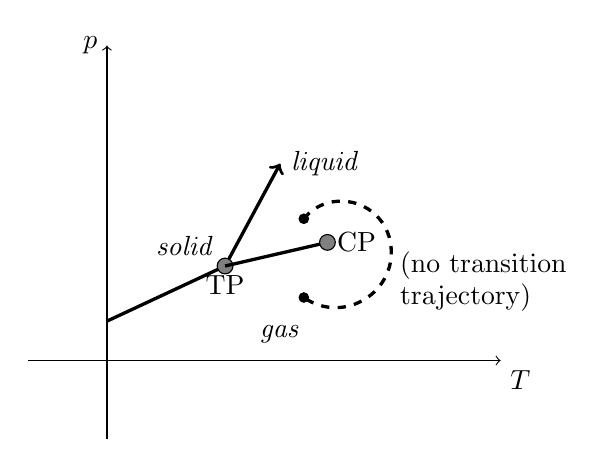
\begin{tikzpicture}[domain=0:6]
\draw[->] (-1,0) -- (5,0)node[below right] {$T$};
\draw[->] (0,-1) -- (0,4)node[left] {$p$};
\draw [very thick] (0,0.5)--(1.5, 1.2)node[above left] {\textit{solid}};
\draw[->, very thick] (1.5, 1.2)--(2.2, 2.5)node[right]{\textit{liquid}};
\draw[fill=gray] (1.5, 1.2) circle (0.1cm);
\draw (1.5, 1.2) node[anchor=north]{TP};
\draw [very thick] (1.5, 1.2)--(2.8, 1.5);
\draw (2.2, 0.1) node[anchor=south]{\textit{gas}};
\draw[fill=gray] (2.8, 1.5) circle (0.1cm);
\draw (2.8, 1.5) node[anchor=west]{CP};
\draw [very thick, dashed] (2.5 ,1.8) to [ curve through ={(2.8, 2) . . (3.6,1.5)  }] (2.5,0.8);
\draw[fill=black] (2.5, 1.8) circle (0.06cm);
\draw[fill=black] (2.5, 0.8) circle (0.06cm);
\draw (3.6,1.2) node[anchor=west]{(no transition};
\draw (3.6,0.8) node[anchor=west]{trajectory)};
\end{tikzpicture}
\end{wrapfigure}
In the liquid-gas-solid phase diagram shown in the figure right, it is possible to choose a path in $p-T$ space which goes from liquid to gas without encountering any singular behaviour in the thermodynamic quantities. This is a reflection of the fact that the liquid and gas states have the same degree of symmetry, whereas a fluid has a higher degree of symmetry than a solid.

\subsubsection{Types of Phase Transition}
Because $f_b[K]$ is everywhere continuous, the phase boundaries must come in two classes: (1) $\partial f_b/\partial K_i$ is discontinuous across a phase boundary. It can be one or more of the derivatives that is discontinuous. In this case, the transition is said to be \textbf{first-order phase transition}\index{first order phase transition}. (2) The only other possibility for non-analytic behavior is that all $\partial f_b/\partial K_i$ are continuous across the phase boundary. If this occurs, the transition is said to be a continuous phase transition.

\subsubsection{Finite-size effects and the correlation length}
If there were perfect instrumental resolution, a change in the physical properties in a finite system would not occur over an infinitesimal interval of the relevant coupling constant, but \textit{would occur over some range}. This phenomenon is an example of a \textbf{finite size effect}\index{finite size effect}.

Loosely speaking, the \textbf{correlation length}\index{correlation length} $\xi$ describes the spatial extent of fluctuations in a physical quantity about the average of that quantity. We might expect that $\xi$ depends upon the coupling constants, in particular temperature. For temperature sufficiently close to $T_c$ that the correlation lentgh of an infinitely large system would exceed characteristic length scale $L$, the behavior of the finite system departs from the ideal behaviour described by $f_b$. To make a rough estimate of when this occurs, let us assume that
\begin{equation}
    \xi\approx\xi_0t^{-2/3}\textit{ where }t\equiv\frac{T-T_c}{T_c}
\end{equation}
with $\xi_0\approx10$\textit{\r A} being the correlation length well away from the critical point. For a system with $L=1 cm$, we find that $\xi=L$ when the reduced temperature $t\approx10^{-11}$. \emph{In this situation, finite size effects would be hard to observe}.

\subsection{The Ising model}
In this model, we consider a lattice in \textit{d} dimensions of sites {\textit{i}} labelled 1 ... N($\Omega$), which we will take to be hypercubic. The DOI are classical spin variables $S_i$, residing on the vertices of the lattice, which takes only two values: up or down. A general form of the Hamiltonian is 
\begin{equation}
\label{isinghamil}
    -H_{\Omega} = \sum_{{i}}H_iS_i+\sum_{ij}J_{ij}S_iS_j
\end{equation}
although we will neglect three and higher spin interactions here. The free energy is given by
\begin{equation}
    F_{\Omega}(T, H_i, J_{ij}) = -k_BTlog(Tre^{-\beta H_{\Omega}})
\end{equation}
The average value of the magnetisation at the site $i$ is obtained by differentiating with respect to the external magnetic field $H_i$:
\begin{equation}
    \frac{\partial F_{\Omega}}{H_i}=-k_BT\frac{1}{Tr e^{-\beta H_{\Omega}}}Tr\frac{S_i}{k_BT}e^{-\beta H_{\Omega}}=-<S_i>_{\Omega}
\end{equation}
Even if we are interested in the situation where there is no magnetic field or one that $H_i=const.$, it is still useful to keep $\sum_{{i}}H_iS_i$ in $H_{\Omega}$ so that formal identities like ones above can be established. At the end of a given calculation, $H_i$ can be set to any desired value. (\textbf{method of sources})\index{mathod of sources}. The partition function can be rewritten according to energy level of $n^{th}$ state, $E_n$:
\begin{equation}
    Z_{\Omega}=\sum_{n=1}^{2^N}exp(-\beta E_n[K])
\end{equation}

\subsection{Analytic properties of the Ising model}
With a uniform external magnetic field $H_i=H$, we can define the magnetisation\index{magnetisation} or magnetic moment per site, $M$:
\renewcommand{\labelenumi}{(\alph{enumi})}
\begin{equation}
    M\equiv\frac{1}{N(\Omega)}\sum_{i=1}^N\langle S_i\rangle=-\frac{\partial f}{\partial H}
\end{equation}
where $f=F_{\Omega}/N$. The principle analytic properties of $f$ are:
\begin{enumerate}
    \item $f<0$,
    \item $f(H,J,T,...)$ is continuous,
    \item $\partial f/\partial T\text{, } \partial f/\partial H$,etc exist almost everywhere,
    \item The entropy per site $S\equiv -\partial f/\partial T\geqslant0$ almost everywhere,
    \item $\partial^2 f/\partial^2 T\leqslant0$,
    \item $\partial^2 f/\partial^2 H\leqslant0$ and thus, susceptibility $\chi_T=-\partial^2 f/\partial^2 H\geqslant0$,
\end{enumerate}
\textbf{Proof of (d)}: Assume existence of derivative for the moment. Then
\begin{equation}
\begin{split}
    -\frac{\partial F_{\Omega}}{\partial T} &= k_Blog Tr e^{-\beta H_{\Omega}}+k_BT\frac{1}{k_BT^2}\frac{Tr H_{\Omega}e^{-\beta H_{\Omega}}}{Tr e^{-\beta H_{\Omega}}}\\
    &=k_B[logZ_{\Omega}+\frac{Tr \beta H_{\Omega}e^{-\beta H_{\Omega}}}{Z_{\Omega}}]\\
    &=-k_BTr(\rho_{\Omega}log\rho_{\Omega})
\end{split}
\end{equation}
where $\rho_{\Omega}\equiv \frac{exp(-\beta H_{\Omega})}{Tr e^{-\beta H_{\Omega}}}$. But equation above is a sum of positive terms, since $0<\rho_{\Omega}<1$ and thus $log \rho_{\Omega}<0$.

The other properties of $f$ listed above are a direct consequence of the property of \textbf{convexity}: $F_{\Omega}$ and $f$ are \textbf{convex functions}\index{convex function} of their arguments $T$, $H$ and $J$.

\subsubsection{Convex functions}
\textbf{Definition:} A function $f(x)$ is said to be \textbf{convex up (down)} in $x$ if $\alpha_1+\alpha_2=1$, we have
\begin{equation}
    \begin{split}
        f(\alpha_1x+\alpha_2y)\geqslant\alpha_1f(x)+\alpha_2f(y)\textit{ (convex up)}\\
        \textit{ or}\\
        f(\alpha_1x+\alpha_2y)\leqslant\alpha_1f(x)+\alpha_2f(y)\textit{ (convex down)}
    \end{split}
\end{equation}
From this definition it can be proved that if $f(x)$ is bounded and convex up (down) then:
\renewcommand{\labelenumi}{(\roman{enumi})}
\begin{enumerate}
    \item $f(x)$ is continuous,
    \item $f(x)$ is differentiable almost everywhere,
    \item $\partial f/\partial x$ is monotonically non-increasing (non-decreasing).
\end{enumerate}

\subsubsection{Convexity and the free energy density}
From \textbf{Holder inequality}\index{Holder inequality}:
\begin{equation}
    \sum_k(g_k)^{\alpha}(h_k)^{\beta}\leqslant(\sum_kg_k)^{\alpha}(\sum_kh_k)^{\beta}
\end{equation}
where $\{g_k\}$ and $\{h_k\}$ are $\geqslant0$, and $\alpha+\beta=1$. Now use the Holder inequality:
\begin{equation}
    Z_{\Omega}(\alpha_1H_1+\alpha_2H_2)\leqslant Z_{\Omega}(H_1)^{\alpha_1}Z_{\Omega}(H_2)^{\alpha_2}
\end{equation}
Taking the logarithm, multiplying by $-k_BT$, dividing by $N$, and taking the thermodynamic limit we find
\begin{equation}
    f(\alpha_1H_1+\alpha_2H_2)\geqslant \alpha_1f(H_1)+\alpha_2f(H_2)
\end{equation}
\subsection{Symmetry properties of the Ising model}
We begin with a trivial lemma: for any function $\phi$ which depends on the spin configuration ${S_i}$,
\begin{equation}
\label{firstlemma}
    \sum_{S_i=\pm 1}\phi(\{S_i\})=\sum_{S_i=\pm1}\phi(\{-S_i\})
\end{equation}
\subsubsection{Time-reversal symmetry}
We now examine the up-down symmetry, called \textbf{$Z_2$ symmetry}\index{Z2 symmetry}. From equation \ref{firstlemma}, the Hamiltonian \ref{isinghamil} can be written as 
\begin{equation}
\label{hamilz2}
    H_{\Omega}(H,J,\{S_i\})=H_{\Omega}(-H,J,\{-S_i\})
\end{equation}
Thus,
\begin{equation}
\begin{split}
\label{t-reveral-sym}
    Z(-H, J,T)&=\sum_{S_i=\pm1}exp[-\beta H_{\Omega}(-H,J,\{S_i\})]\\
    &=\sum_{S_i=\pm1}exp[-\beta H(-H,J,\{-S_i\})]\\
    &=\sum_{S_i=\pm1}exp[-\beta H(H,J,\{S_i\})]\textit{ from eq.\ref{hamilz2}}\\
\end{split}
\end{equation}
Thus the free energy density is even in $H$: $f(H,J,T)=f(-H,J,T)$.

\subsubsection{Sub-lattice symmetry}
When $H=0$, there is \textbf{sub-lattice symmetry}\index{sub-lattice symmetry}. We divide our hypercubic lattice up into two interpenetrating \textbf{sub-lattices}, which we shall call $A$ and $B$. In the Hamiltonian
\begin{equation}
    H_{\Omega}(0, J,\{S_i\})=-J\sum_{\langle ij \rangle}S_iS_j
\end{equation}
the spins on sub-lattice $A$ only interact with spins on sub-lattice $B$ and \emph{vice versa}, so we can trivially re-write the Hamiltonian as
\begin{equation}
\label{subhamil}
    H_{\Omega}(0, J,\{S^A_i\},\{S^B_i\})=-J\sum_{\langle ij\rangle}S^A_iS^B_j
\end{equation}
The Hamiltonian, written as in eqn. \ref{subhamil}, exhibits the symmetry
\begin{equation}
\begin{split}
    H_{\Omega}(0, -J,\{S^A_i\},\{S^B_i\})&=H_{\Omega}(0, J,\{-S^A_i\},\{S^B_i\})\\
    &=H_{\Omega}(0, J,\{S^A_i\},\{-S^B_i\})
\end{split}
\end{equation}
and
\begin{equation}
\begin{split}
    Z_{\Omega}(0,-J,T)&=\sum_{\{S^A\}}\sum_{\{S^B\}} e^{-\beta H_{\Omega}(0,-J, S_i^A,S_i^B)}\\
    &=\sum_{\{S^A\}}\sum_{\{S^B\}} e^{-\beta H_{\Omega}(0,J, -S_i^A,S_i^B)}\\
    &=Z_{\Omega}(0,J,T)
\end{split}
\end{equation}
Thus, we obtain the second symmetry property of the free energy density:
\begin{equation}
    f(0, J, T)=f(0,-J,T)
\end{equation}
In zero field, the ferromagnetic Ising model (J>0) and the anti-ferromagnetic Ising model (J<0) on a hypercubic lattic have the \emph{same thermodynamics}. This conclusion relies on the fact that a hypercubic lattice is \textbf{bipartite}\index{bipartite}: it can be subdivided into two equivalent sub-lattice. The theorem does not apply on a triangular lattice, which is not bipartite. On the triangular lattice, it is not possible to simultaneously minimize all the interactions. This phenomenon is an example of \textbf{frustration}\index{frustration}.

\subsection{Existence of phase transitions}
How do we construct the phase diagram of a particular system? One of the most useful techniques is the so-called \textbf{energy-entropy argument}\index{energy-entropy argument}. At high temperature, the free energy is minimized by minimizing $S$. At low temperature, the free energy is minimized by minimising $E$. \textit{if the macroscopic states of the system obtained by these two procedures are different, then we conclude that at least one phase transition has occurred at some intermediate temperature}.

\textbf{Lemma}: If the energy $E$ is the sum of a number of terms dependent upon the spin configuration $[S]$:
\begin{equation}
    E=\sum_{\lambda}E_{\lambda}[S]
\end{equation}
then
\begin{equation}
    min_{[S]}E\geqslant\sum_{\lambda}min_{[S]}E_{\lambda}[S]
\end{equation}
The ground state is any state for which the equality is satisfied.
\subsubsection{Zero temperature phase diagram}
\begin{wrapfigure}{l}{6cm}
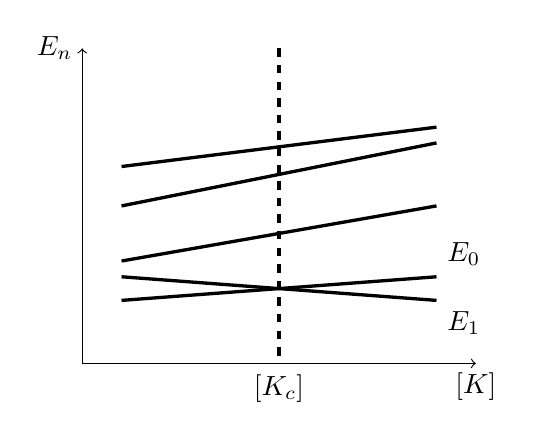
\begin{tikzpicture}[domain=0:6]
\draw[->] (0,0) -- (5,0)node[below] {$[K]$};
\draw[->] (0,0) -- (0,4)node[left] {$E_n$};
\draw [very thick] (0.5,2.5)--(4.5, 3.0);
\draw [very thick] (0.5, 2.0)--(4.5, 2.8);
\draw [very thick] (0.5, 1.3)--(4.5, 2.0);
\draw [very thick] (0.5, 1.1)--(4.5, 0.8)node[below right]{$E_1$};
\draw [very thick] (0.5, 0.8)--(4.5, 1.1) node[above right]{$E_0$};
\draw[dashed, very thick] (2.5, 4)--(2.5, 0) node[below]{$[K_c]$};
\end{tikzpicture}
\end{wrapfigure}
If we can map out the energy levels as a function of [K], as sketched left. It may happen that as the coupling constants pass through the set of values denoted by [$K_c$] the first excited state of the system. This will usually generate a first order transition, because \textbf{there will be a discontinuity in $\partial E/\partial K_i$}. This mechanism for a \textbf{zero temperature phase transition }is known as \textbf{level crossing}.\index{level crossing} The non-analytic behaviour is permitted to occur in this case, not because $N\rightarrow\infty$, but because $\beta\rightarrow\infty$.

\subsubsection{Phase diagram at non-zero temperature: d=1}
In d=1 for $T>0$ there is no \textbf{long range order}(i.e. no ferromagnetic state), whereas for d=2, long range order can exist above $T=0$, with a transition at $T_c>0$ to a paramagnetic state. In the preceding section, we found that at zero temperature, there are two possible phases at zero field: all spins up and all spins down. Consider the spin up phase $\uparrow\uparrow\uparrow...\uparrow\uparrow\uparrow$. As the temperature is raised above zero, the uncorrelated flipping of a finite number of spins, $n$, cannot destroy long range order. Only a large fraction of spins flipping, $f$, could destroy long range order.
\begin{equation}
    lim_{N(\Omega)\rightarrow\infty}\frac{N-fN}{N}<1
\end{equation}
In the ordered state the entropy is zero, so the free energy is just $F_N=-NJ$. Now consider the state with 2 domain
\[\uparrow\uparrow...\uparrow\wr\downarrow...\downarrow\downarrow\]
The interface \(\wr\) has cost energy. In fact,
\begin{equation}
    E_{N}=-NJ+2J=-(N-1)J+J
\end{equation}
and the entropy becomes $S_N=k_BlogN$. Hence, the free energy difference between the state with an interface and the state with all spins up is
\begin{equation}
    \Delta F=2J-k_BTlogN
\end{equation}
\textbf{For and $T>0$, $\Delta F\rightarrow-\infty$ as $N\rightarrow\infty$.} \emph{The system can lower the free energy by creating a domain wall for any temperature $T>0$.} Thus, the long range order state is unstable towards thermal fluctuations for $T>0$.

If the interaction $J_{ij}$ between spins at $r_i$ and $r_j$ varies as
\begin{equation}
    J_{ij}=\frac{J}{|r_i-r_j|^{\sigma}}
\end{equation}
then long range order may persist for $0<T<T_c$ as long as $1\leqslant\sigma\leqslant2$. For $\sigma<1$, the thermodynamic limit does not exist. For $\sigma>2$, the interaction qualifies as being short-ranged, and the argument for the destruction of long range order for $T>0$ applies.

\subsubsection{Phase diagram at non-zero temperature: d=2}
Suppose the border between the flipped spins and the up spins contains $n$ bonds. Then the energy difference between the state with a domain and one with complete long range order is $\Delta E\sim 2Jn$. If the co-ordination number of the number of the lattice is $z$, then we can estimate the entropy as:$\Delta S\sim k_Bnlog(z-1)$. Thus, the change in free energy due to a domain whose boundary contains $n$ bonds is
\begin{equation}
    \Delta F_n=[2J-(log(z-1))k_BT]n
\end{equation}
At the thermodynamic limit, $n\rightarrow\infty$, the behaviour of $\Delta F_n$ in this limit depends upon the temperature. If
\begin{equation}
    T>T_c\equiv\frac{2J}{k_Blog(z-1)}
\end{equation}
then $\Delta F\rightarrow-\infty$ as $n\rightarrow\infty$ and the system is unstable towards the formation of domains. For $0<T<T_c$, $\Delta F$ is minimized by $n\rightarrow0$, the system exhibits a net magnetization M. In the absence of an applied field, this phenomenon is referred to as \textbf{spontaneous magnetization}\index{spontaneous magnetization}.

Note that the transition temperature depends on coordination number $z$, and therefore on the type of lattice. \emph{The transition temperature is not a unversal quantity}.

\subsubsection{Impossibility of phase transition}
From equation \ref{t-reveral-sym}, we know that 
\begin{equation}
    \begin{array}{l}{ F _ { \Omega } ( H , J , T ) = F _ { \Omega } ( - H , J , T ) }\\{ M ( H ) M _ { \Omega } ( H ) = - \frac { \partial F _ { \Omega } ( H ) } { \partial H } }\\{ = - \frac { \partial F _ { \Omega } ( - H ) } { \partial H } }\\{ = \frac { \partial F _ { \Omega } ( - H ) } { \partial ( - H ) } }\\{ = - N ( \Omega ) M _ { \Omega } ( - H ) }\\{ M _ { \Omega } ( H ) = - M _ { \Omega } ( - H ) }\end{array} 
\end{equation}
At $H=0$ we must have
\begin{equation}
\label{impossible-theorem}
    M_{\Omega}(0) = -M_{\Omega}=0
\end{equation}
This "impossibility" theorem\index{impossibility theorem} shows that the magnetisation in zero external field must be zero, ant the phase transition become impossible. In fact, \textbf{the symmetry of Hamiltonian at thermodynamic limit is broken.}

\subsection{Spontaneous symmetry breaking}
The argument of $M(0)=0$ is correct for \textbf{a finite system}. It fails in the thermodynamic limit, because $f(H)$ can develop a discontinuity in its first derivative $\partial f/\partial H$. The condition $f(H)=f(-H)$ does not imply $M(0)=0$ unless \textbf{we assume $f(H)$ is smooth at $H=0$}.



\tikzset{every picture/.style={line width=0.75pt}} %set default line width to 0.75pt        

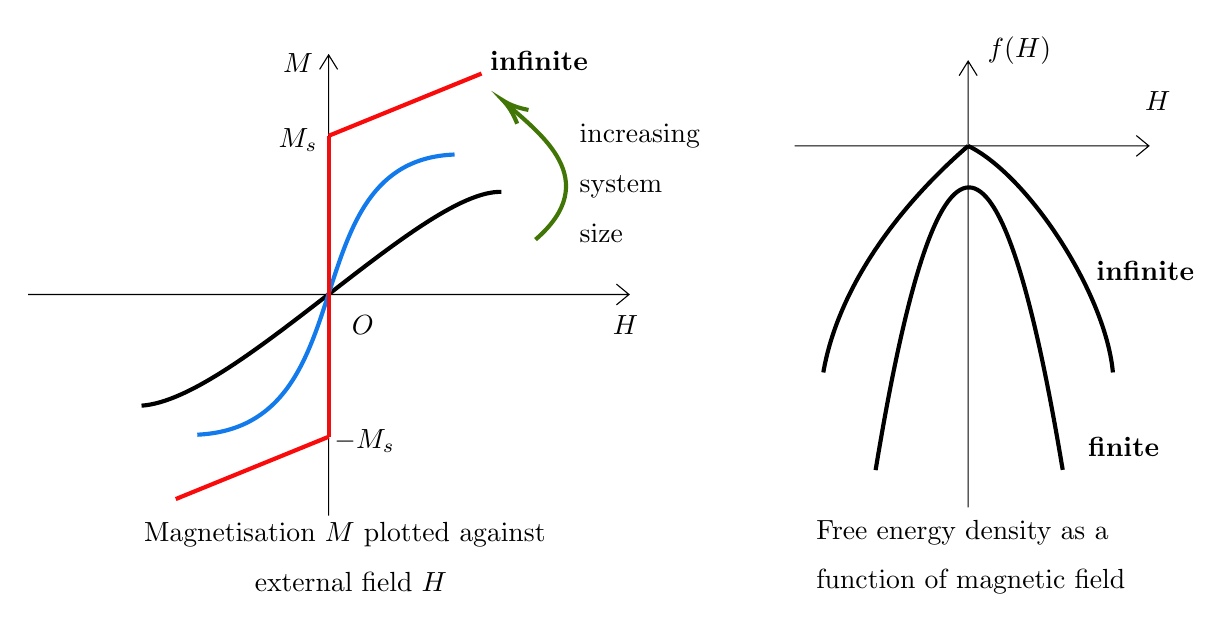
\begin{tikzpicture}[x=0.65pt,y=0.75pt,yscale=-1,xscale=1]
\path (0,295); %set diagram left start at 0, and has height of 295

%Shape: Axis 2D [id:dp5559015927211374] 
\draw  (-4,143.44) -- (330,143.44)(163,28) -- (163,250) (323,138.44) -- (330,143.44) -- (323,148.44) (158,35) -- (163,28) -- (168,35)  ;
%Curve Lines [id:da8118404892921705] 
\draw [line width=1.5]    (59,197) .. controls (111,194) and (215,93) .. (259,94) ;


%Curve Lines [id:da656011700434274] 
\draw [color={rgb, 255:red, 19; green, 122; blue, 235 }  ,draw opacity=1 ][line width=1.5]    (90,211) .. controls (186,207) and (141,79) .. (233,76) ;


%Straight Lines [id:da2869018515069013] 
\draw [color={rgb, 255:red, 250; green, 11; blue, 11 }  ,draw opacity=1 ][line width=1.5]    (78,242) -- (163,212) ;


%Straight Lines [id:da15135394123831747] 
\draw [color={rgb, 255:red, 238; green, 15; blue, 15 }  ,draw opacity=1 ][line width=1.5]    (163,67) -- (163,212) ;


%Straight Lines [id:da4982177217220094] 
\draw [color={rgb, 255:red, 250; green, 11; blue, 11 }  ,draw opacity=1 ][line width=1.5]    (163,67) -- (248,37) ;


%Curve Lines [id:da791784529929195] 
\draw [color={rgb, 255:red, 65; green, 117; blue, 5 }  ,draw opacity=1 ][line width=1.5]    (278,117) .. controls (316.4,88.2) and (280.15,65.85) .. (262.15,51.72) ;
\draw [shift={(260,50)}, rotate = 399.47] [color={rgb, 255:red, 65; green, 117; blue, 5 }  ,draw opacity=1 ][line width=1.5]    (14.21,-4.28) .. controls (9.04,-1.82) and (4.3,-0.39) .. (0,0) .. controls (4.3,0.39) and (9.04,1.82) .. (14.21,4.28)   ;

%Shape: Axis 2D [id:dp7437264409166084] 
\draw  (422,71.85) -- (619,71.85)(518.53,31) -- (518.53,246) (612,66.85) -- (619,71.85) -- (612,76.85) (513.53,38) -- (518.53,31) -- (523.53,38)  ;
%Curve Lines [id:da009234981277251197] 
\draw [line width=1.5]    (438,181) .. controls (446,141) and (478.53,101.85) .. (518.53,71.85) ;


%Curve Lines [id:da44036554290303564] 
\draw [line width=1.5]    (599,181) .. controls (595,143) and (552,86) .. (518.53,71.85) ;


%Shape: Parabola [id:dp026738883579881967] 
\draw  [line width=1.5]  (571.09,227.93) .. controls (536.2,46.44) and (501.53,46.48) .. (467.08,228.06) ;

% Text Node
\draw (280,31) node  [align=left] {\textbf{infinite}};
% Text Node
\draw (336,90) node  [align=left] {increasing\\system\\size};
% Text Node
\draw (328,158) node  [align=left] {$\displaystyle H$};
% Text Node
\draw (146,32) node  [align=left] {$\displaystyle M$};
% Text Node
\draw (146,69) node  [align=left] {$\displaystyle M_{s}$};
% Text Node
\draw (183,214) node  [align=left] {$\displaystyle -M_{s}$};
% Text Node
\draw (182,158) node  [align=left] {$\displaystyle O$};
% Text Node
\draw (617,132) node  [align=left] {\textbf{infinite}};
% Text Node
\draw (605,217) node  [align=left] {\textbf{finite}};
% Text Node
\draw (547,26) node   {$f( H)$};
% Text Node
\draw (624,50) node   {$H$};
% Text Node
\draw (520,270) node [scale=1] [align=left] {Free energy density as a\\ function of magnetic field};
% Text Node
\draw (172,270) node [scale=1] [align=left] {Magnetisation $\displaystyle M$ plotted against \\ \ \ \ \ \ \ \ \ \ \ \ \ external field $\displaystyle H$};

\end{tikzpicture}

However, \textbf{none of the properties of $f(H)$ guarantee that smoothness occurs.} The figure above shows that we can evade the consequence of the "impossibility theorem" by creating the discontinuity near $H=0$. From the graph of magnetisation M versus $H$, we see that $M_s$, the spontaneous magnetisation is given by
\begin{equation}
    \begin{array}{l}{ M _ { s } = \lim _ { H \rightarrow 0 ^ { + } } - \frac { \partial f ( H ) } { \partial H } }\\{ - M _ { s } = \lim _ { H \rightarrow 0 ^ { - } } - \frac { \partial f ( H ) } { \partial H } }\end{array} 
\end{equation}
Notice that the limits: (a)$N\rightarrow\infty$ and (b)$H\rightarrow0$ \textbf{do not commute:}
\begin{equation}
    \begin{array} { l } {  \text{lim}_{N \rightarrow \infty}  \lim _ { H \rightarrow 0 } \frac { 1 } { N ( \Omega ) } \frac { \partial F _ { \Omega } ( H ) } { \partial H } = 0 } \\ { \lim _ { H \rightarrow 0 } \lim _ { N \rightarrow \infty } \frac { 1 } { N ( \Omega ) } \frac { \partial F _ { \Omega } ( H ) } { \partial H } \neq 0 } \end{array} 
\end{equation}
Notice also $M_s=f(T)$: at zero temperature, we know that $M_s$ should be unity as the spins will be all up or all down. As $T\rightarrow T_c$, the value of the spontaneous magnetisation is reduced.

This set of phenomena is referred to as \textbf{spontaneous sysmmetry breaking}\index{symmetry breaking!spontaneous}. When H=0:
\begin{equation}
    H _ { \Omega } [ \{ S _ { i } \} ] = H _ { \Omega } [ \{ - S _ { i } \} ]
\end{equation}
\textbf{Even though the Hamiltonian is invariant under $\{S_i\}\rightarrow\{-S_i\}$, the statistical expectation values are not invariant under time-reversal symmetry $\langle S_i\rangle\neq0$} and
\begin{equation}
    M=\lim _ { N arrow \infty } \frac { 1 } { N ( \Omega ) } \sum _ { i } \langle S _ { i } \rangle\neq0
\end{equation}
The use of the word "spontaneous" in the above definition is to distinguish this phenomenon from \emph{the appearance of magnetisation in the presence of an external field.}

\subsubsection{Probability distribution}
If the probability of finding the system in a state is given by the \textbf{Boltzmann distribution}
\begin{equation}
    \begin{split}
        P _ { \Omega } ( \{ S _ { i } \} ) = \frac { \exp ( - \beta H _ { \Omega } ( \{ S _ { i } \} ) ) } { Z _ { \Omega } }\\
        \langle S _ { i } \rangle \equiv \operatorname { Tr } P _ { \Omega } ( \{ S _ { i } \} ) S _ { i } = 0\\
    \end{split}
\end{equation}
since the distribution is even and $S_i$ is odd. This is a restatement of "impossible theorem".  \textbf{In the thermodynamic limit, the probability distribution is not necessarily given by the Boltzmann distribution.}

Now apply an external field $H$. If two configurations of the system, A and B, are related by \emph{time-reversal symmetry}, the probability ratio of these two state is:
\begin{equation}
     \frac { P _ { A } } { P _ { B } } = \frac { e ^ { - \beta ( - H N ( \Omega ) M ) } } { e ^ { - \beta ( H N ( \Omega ) M ) } } = e^{2\beta HNM}
\end{equation}
Taking the limit $N ( \Omega )\rightarrow\infty$, for $H>0$, gives
\begin{equation}
    \frac{P_B}{P_A}\rightarrow0
\end{equation}
and thus the system must be state A, $+M$. Similarly, if $H\rightarrow0^-$, the system has the magnetisation $-M$. To explain spontaneous magnetisation in the thermodynamic limit, in zero field, we notice that the use of the limit $H\rightarrow 0^+$ is equivalent to setting $H=0$ but \textbf{using a restricted ensemble in which microstates contributing to $-M_s$ are not included}. The probability distribution for a system after the thermo limit has been taken is identically zero for all states whose magnetisation is negative.

\subsubsection{Continuous symmetry}
The fact that the Ising model has a \textbf{discrete symmetry}\index{symmetry!discrete} means that the width of the domain walls must be \textit{finite.} However, things change if the spin obey a \textbf{continuous symmetry}\index{symmetry!continuous} (e.g.,\textbf{Heisenberg ferromagnet}). One way for this to occur is if the spins are vectors, allowed to point in \textit{all directions}:
\begin{equation}
    H _ { \Omega } [ \{ S _ { i } \} ] = - \sum J _ { i j } S _ { i } \cdot S _ { j } - \sum H _ { i } \cdot s _ { i }
\end{equation}
Suppose $R(\theta)$ is a rotation matrix which rotates a vector in space by an angle $\theta$ about arbitrary direction. The energy defined above is invariant under the \textbf{simultaneous rotation of all the spins by an angle $\theta$}(\textbf{rotationally invariant}, $O(3)$, in 3D space\index{O(3) symmetry}):
\begin{equation}
    H _ { \Omega } [ \{ R ( \theta ) S _ { i } \} ] = H _ { \Omega } [ \{ S _ { i } \} ]
\end{equation}

The continuous rotational symmetry is spontaneously broken in the state of long range order. To compensate for the increased entropy due to the larger dimensionality of the order parameter,\textbf{an increased energy is required if there is to be long range order in the Heisenberg model at $T>0$.} This can be achieved by \emph{increasing the dimensionality of the lattice.}

\subsection{Ergodicity breaking}
\textbf{What are the consequences of spontaneous symmetry breaking for the dynamics?} In stat. mech., the time average of any observables $A{\eta_i}$ is given by:
\begin{equation}
    \begin{array} { l } { \langle A \rangle \equiv \lim _ { t \rightarrow \infty } \frac { 1 } { t } \int _ { 0 } ^ { t } A \{ \eta _ { i } ( t ^ { \prime } ) \} d t ^ { \prime } } \\  { \langle A \rangle = \int \prod _ { i } d \eta _ { i } P _ { \text { eqm } } ( \{ \eta _ { i } \} ) A \{ \eta _ { i } \} } \end{array} 
\end{equation}
where $\eta$ are dynamic DOI as functions of time, $P_{eqm}(\eta_i)$ is the \emph{equilibrium probability distribution of $\{\eta_i\}$}. These equations are based on the \textbf{ergodic hypothesis}\index{ergodic hypothesis}: as $t\rightarrow\infty$, $\eta_i(t)$ comes arbitrarily close to every possible configuration of the $\eta_i$ allowed by energy conservation.

In the thermodynamic limit, the lifetime of a cluster of spins will rapidly grow very large (e.g.,$\tau\sim exp[N^{(d-1)/d}]$), so that the \textbf{initial condition} determines whether or not the magnetisation is positive or negative. The system is effectively \textit{trapped in one or the other region of configuration or phase space}. This is known as \textbf{ergodicity breaking}\index{ergodicity breaking}.

\subsubsection{Illustrative example}
Consider a system with DOI $\{c_i\}$ ($i$=1,...,N) and a Hamiltonian $H_{\lambda}\{c_i\}$. If the system is translationally invariant:
\begin{equation}
    H _ { \lambda } \{ c _ { i } \} = H _ { \lambda } \{ c _ { i } + a \}
\end{equation}
The parameter $\lambda$ is supposed to represent all the parameters or coupling constants in the Hamiltonian. Now suppose that we are interested in computing the expectation value of the function $f_i(\boldsymbol{k})$, $\boldsymbol{k}\neq0$:
\begin{equation}
    f _ { i } ( k ) = \exp ( i k \cdot c _ { i } ) 
\end{equation}
The function serves as our order parameter. It has a simple interpretation:\textbf{when summed over $i$, it is the Fourier transform of the density}: $\rho(r)=\sum_i\delta(r-c_i)$. Thus, we expect that for $\lambda>\lambda_c$, $\langle f_i(k)\rangle=0$, whilst for $\lambda<\lambda_c$,$\langle f_i(k)\rangle\neq0$. To be more precise:
\begin{equation}
    \langle f _ { i } ( k ) \rangle _ { \sigma } = \frac { \operatorname { Tr } _ { \sigma } f _ { i } ( k ) \exp ( - \beta H _ { \lambda } \{ c _ { i } \} ) } { \operatorname { Tr } _ { c } \exp ( - \beta H _ { \lambda } \{ c _ { i } \} ) }
\end{equation}
where $\sigma$ denotes the microstates included in the trace operation.

What would happen when $\lambda=\lambda_c$? The fact that $\langle f _ { i } ( k ) \rangle _ { \sigma }$ becomes non-zero means that \textbf{the density of the system is not simply a constant in space, as it is for $\lambda>\lambda_c$. Thus the transition is associated with some ordering of the particles in space--solidification}\index{solidification}.

To internalize the argument above, think about the XRD of solid, and liquid. We only got peak patterns for solid, indicating $\langle f _ { i } ( k ) \rangle _ { \sigma }\neq 0$.

To proceed, we must first specify which microstates should be included in $\sigma$. If all possible microstates are included, then because of the translational invariance:
\begin{equation}
    \langle f _ { i } ( k ) \rangle _ { \sigma } = e ^ { i k \cdot a } \langle f _ { i } ( k ) \rangle _ { \sigma }
\end{equation}
and hence $\langle f _ { i } ( k ) \rangle _ { \sigma }= 0$ regardless of the value of $\lambda$. Therefore, it is only if the residual set $\sigma$ is not invariant under the symmetry can acquire a non-zero value of the order parameter.\textbf{The requirement that the set of microstates included in the trace be restricted for $\lambda<\lambda_c$ is ergodicity breaking}.

In summary, there are two complementary ways of looking at spontaneous symmetry breaking:(i) Method of small fields:$H\rightarrow0^+$ etc. (ii) Ergodicity breaking and the restricted ensemble.

\subsubsection{Symmetry and its implications for ergodicity breaking}
Let $\lambda_2$ be a set of microstates generated from the set $\lambda_1$ by some member T of the translational transformations $T_a$:$\lambda_2=T(\lambda_1)$, $H(Tc_i)=H(c_i)$, $Z_2=Z_1$. Thus, $\langle f _ { i } ( k ) \rangle _ { \sigma2 }=e^{ik\cdot a}\langle f _ { i } ( k ) \rangle _ { \sigma1 }$. Hence, we conclude that \textbf{if ergodicity is broken so that a certain order parameter is non-zero in some set $\sigma$ of microstates in phase space, then the order parameter will attain a non-zero value in all other sets of microstates related to $\sigma$ by applying the symmetry of the Hamiltonian that has been spontaneously broken}.



\tikzset{every picture/.style={line width=0.75pt}} %set default line width to 0.75pt        

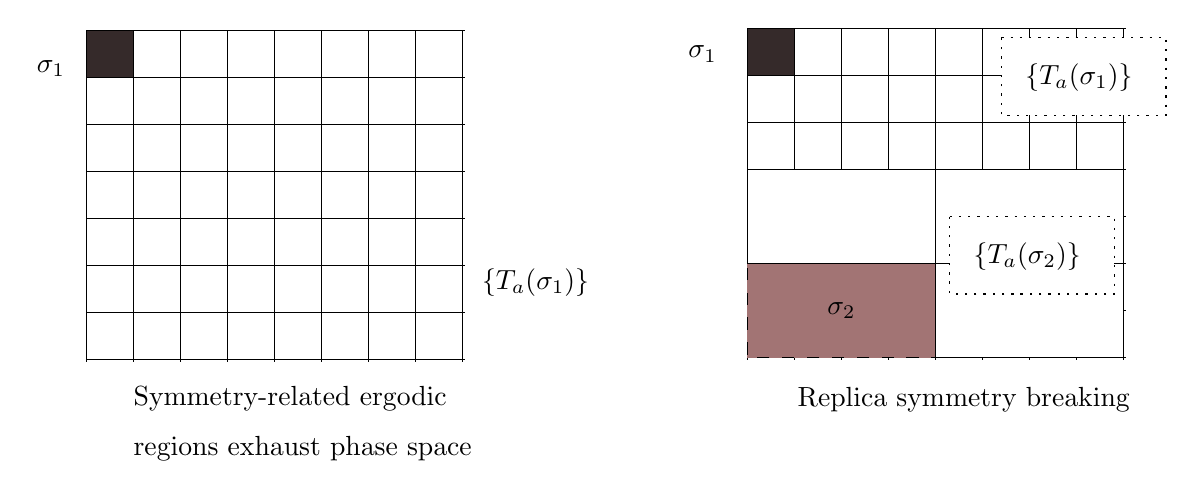
\begin{tikzpicture}[x=0.85pt,y=0.85pt,yscale=-1,xscale=1]
%uncomment if require: \path (0,192); %set diagram left start at 0, and has height of 192

%Shape: Grid [id:dp9462499325366089] 
\draw  [draw opacity=0] (33,15) -- (194,15) -- (194,156) -- (33,156) -- cycle ; \draw   (33,15) -- (33,156)(53,15) -- (53,156)(73,15) -- (73,156)(93,15) -- (93,156)(113,15) -- (113,156)(133,15) -- (133,156)(153,15) -- (153,156)(173,15) -- (173,156)(193,15) -- (193,156) ; \draw   (33,15) -- (194,15)(33,35) -- (194,35)(33,55) -- (194,55)(33,75) -- (194,75)(33,95) -- (194,95)(33,115) -- (194,115)(33,135) -- (194,135)(33,155) -- (194,155) ; \draw    ;
%Shape: Rectangle [id:dp7331769696990961] 
\draw  [fill={rgb, 255:red, 53; green, 42; blue, 42 }  ,fill opacity=1 ] (33,15) -- (53,15) -- (53,35) -- (33,35) -- cycle ;
%Shape: Grid [id:dp388435085632994] 
\draw  [draw opacity=0] (314,14) -- (475,14) -- (475,155) -- (314,155) -- cycle ; \draw   (314,14) -- (314,155)(334,14) -- (334,155)(354,14) -- (354,155)(374,14) -- (374,155)(394,14) -- (394,155)(414,14) -- (414,155)(434,14) -- (434,155)(454,14) -- (454,155)(474,14) -- (474,155) ; \draw   (314,14) -- (475,14)(314,34) -- (475,34)(314,54) -- (475,54)(314,74) -- (475,74)(314,94) -- (475,94)(314,114) -- (475,114)(314,134) -- (475,134)(314,154) -- (475,154) ; \draw    ;
%Shape: Rectangle [id:dp8763618826392132] 
\draw  [fill={rgb, 255:red, 162; green, 116; blue, 116 }  ,fill opacity=1 ][dash pattern={on 4.5pt off 4.5pt}] (314,114) -- (394,114) -- (394,154) -- (314,154) -- cycle ;
%Shape: Rectangle [id:dp9501695179727356] 
\draw  [fill={rgb, 255:red, 255; green, 255; blue, 255 }  ,fill opacity=1 ] (394,114) -- (474,114) -- (474,154) -- (394,154) -- cycle ;
%Shape: Rectangle [id:dp6403102931712145] 
\draw  [fill={rgb, 255:red, 255; green, 255; blue, 255 }  ,fill opacity=1 ] (314,74) -- (394,74) -- (394,114) -- (314,114) -- cycle ;
%Shape: Rectangle [id:dp4144077482991442] 
\draw  [fill={rgb, 255:red, 255; green, 255; blue, 255 }  ,fill opacity=1 ] (394,74) -- (474,74) -- (474,114) -- (394,114) -- cycle ;
%Shape: Rectangle [id:dp6243691792039068] 
\draw  [fill={rgb, 255:red, 53; green, 42; blue, 42 }  ,fill opacity=1 ] (314,14) -- (334,14) -- (334,34) -- (314,34) -- cycle ;
%Shape: Rectangle [id:dp6113510819459621] 
\draw  [fill={rgb, 255:red, 255; green, 255; blue, 255 }  ,fill opacity=1 ][dash pattern={on 0.84pt off 2.51pt}] (422,18) -- (492,18) -- (492,51) -- (422,51) -- cycle ;
%Shape: Rectangle [id:dp36532529079191833] 
\draw  [fill={rgb, 255:red, 255; green, 255; blue, 255 }  ,fill opacity=1 ][dash pattern={on 0.84pt off 2.51pt}] (400,94) -- (470,94) -- (470,127) -- (400,127) -- cycle ;

% Text Node
\draw (18,31) node   {$\sigma _{1}$};
% Text Node
\draw (224,122) node  [align=left] {$\displaystyle \{T_{a}( \sigma _{1})\}$};
% Text Node
\draw (295,25) node   {$\sigma _{1}$};
% Text Node
\draw (455,35) node  [align=left] {$\displaystyle \{T_{a}( \sigma _{1})\}$};
% Text Node
\draw (433,111) node  [align=left] {$\displaystyle \{T_{a}( \sigma _{2})\}$};
% Text Node
\draw (354,134) node   {$\sigma _{2}$};
% Text Node
\draw (125,182) node  [align=left] {Symmetry-related ergodic \\regions exhaust phase space};
% Text Node
\draw (406,172) node  [align=left] {Replica symmetry breaking};


\end{tikzpicture}

We have shown that \textbf{spontaneous symmetry breaking generates disjoint ergodic regions} in phase space, we must logically allow, in principle, for the possibility that the symmetry-related ergodic region in phase space do not \textbf{exhaust phase space}. If an ergodic region and its symmetry-related counterparts do exhaust phase space, then there is only one way for the solid state to exist, corresponding to the microstates contained within the region. If there are, for example, two sets $\lambda_1$ and $\lambda_2$, each with their symmetry-related counterparts, which are required to exhaust phase space, then we conclude that \textbf{there are two ways for the solid state to exist, one corresponding to $\lambda_1$, the other to $\lambda_2$}. The latter possibility is referred to as \textbf{replica symmetry breaking}\index{symmetry breaking!replica}.(broken symmetry is replicated)

\subsubsection{Possible forms for possibility distribution of overlap}
When the replica symmetry breaking happens, it is usually complicated to differentiate different phase space region, both symmetry related and non-symmetry related. To obviate these difficultis, we can employ the concept of \textbf{overlap}\index{overlap} between the region $\sigma$ and $\sigma^{\prime}$, $q^{\sigma\sigma^{\prime}}$. Its probability distribution is:
\begin{equation}
    P(q)\equiv\sum_{\sigma\sigma^{\prime}}\omega^{\sigma}\omega^{\sigma^{\prime}}\delta(q-q^{\sigma\sigma^{\prime}})
\end{equation}
where
\begin{equation}
    \omega^{\sigma}\equiv\frac{Z_{\sigma}}{\sum_{\tau}Z_{\tau}}
\end{equation}
and the overlap of two phase space regions is defined as
\begin{equation}
    \begin{array}{c}{q^{\sigma \sigma^{\prime}} \equiv \lim _{N(\Omega) \rightarrow \infty}\left|\frac{1}{N(\Omega)} \sum_{i=1}^{N(\Omega)} m_{i}^{\sigma} m_{i}^{q^{\prime}}\right|} \\ {m_{i}^{\sigma}=\frac{1}{Z_{\sigma}} \operatorname{Tr}_{\sigma} S_{i} e^{-\beta H_{\Omega}}}\end{array}
\end{equation}
The overlap has several desirable features. It is zero in the paramagnetic phase, but may be non-zero for appropriate choices of $\sigma$ and $\sigma'$ in the spin glass phase. In particular, $q^{\sigma \sigma} \neq 0$. If ergodic region $\sigma_1'$ is the same as ergodic region $\sigma_1$ , but all the spins are flipped (i.e. $\sigma_1$ are $\sigma_1'$ related by time-reversal symmetry), then $q^{\sigma \sigma_{1}}=q^{\sigma \sigma_{1}^{\prime}}$ , showing that the overlap does not favour any particular ergodic region over its symmetry-related counterparts.
\tikzset{every picture/.style={line width=0.75pt}} %set default line width to 0.75pt        

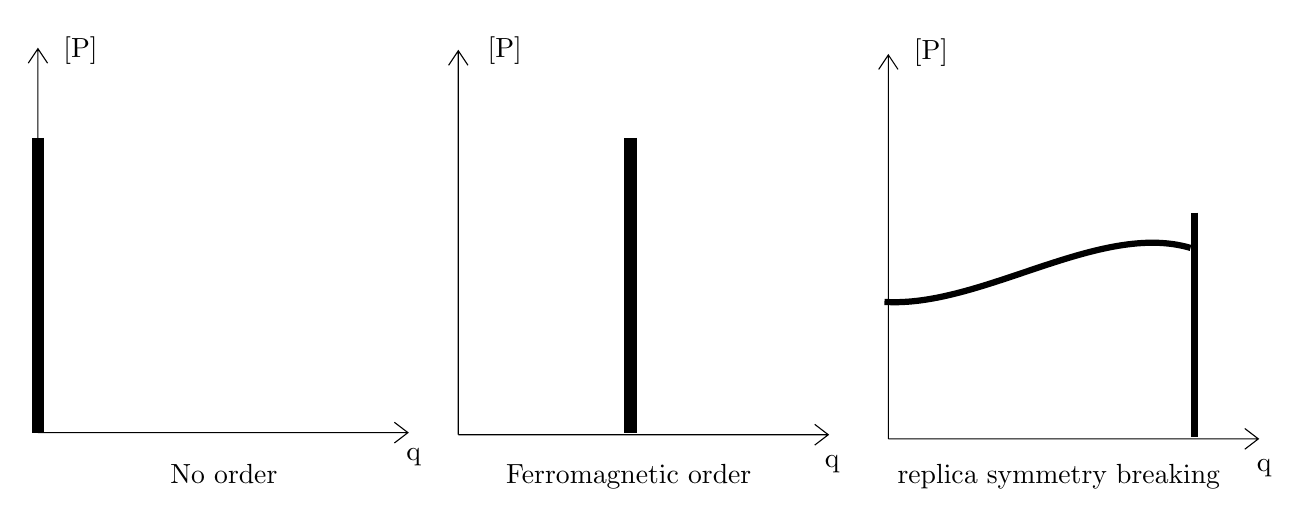
\begin{tikzpicture}[x=0.7pt,y=0.75pt,yscale=-1,xscale=1]
%uncomment if require: \path (0,300); %set diagram left start at 0, and has height of 300

%Shape: Axis 2D [id:dp4398561135234478] 
\draw  (12,249) -- (203,249)(12,64) -- (12,249) -- cycle (196,244) -- (203,249) -- (196,254) (7,71) -- (12,64) -- (17,71)  ;
%Shape: Axis 2D [id:dp7828317466085237] 
\draw  (229,250) -- (420,250)(229,65) -- (229,250) -- cycle (413,245) -- (420,250) -- (413,255) (224,72) -- (229,65) -- (234,72)  ;
%Shape: Axis 2D [id:dp8373035026435443] 
\draw  (451,252) -- (642,252)(451,67) -- (451,252) -- cycle (635,247) -- (642,252) -- (635,257) (446,74) -- (451,67) -- (456,74)  ;
%Straight Lines [id:da2512526838445679] 
\draw [line width=4.5]    (12,107) -- (12,249) ;


%Straight Lines [id:da8681762451774699] 
\draw [line width=4.5]    (318,107) -- (318,249) ;


%Straight Lines [id:da9977299646388169] 
\draw [line width=2.25]    (609,143) -- (609,251) ;


%Curve Lines [id:da06866257233439232] 
\draw [line width=2.25]    (449,186) .. controls (499,189) and (560,147) .. (607,160) ;



% Text Node
\draw (34,65) node  [align=left] {[P]};
% Text Node
\draw (253,65) node  [align=left] {[P]};
% Text Node
\draw (473,66) node  [align=left] {[P]};
% Text Node
\draw (206,261) node  [align=left] {q};
% Text Node
\draw (422,264) node  [align=left] {q};
% Text Node
\draw (645,266) node  [align=left] {q};
% Text Node
\draw (108,269) node  [align=left] {No order};
% Text Node
\draw (317,270) node  [align=left] {Ferromagnetic order};
% Text Node
\draw (539,270) node  [align=left] {replica symmetry breaking};


\end{tikzpicture}

\subsection{Equivalence in statistical mechanics}
\begin{itemize}
    \item Exact equivalence: exact mapping of one model partition function of the two models. For instance, Ising model to lattice gas equivalence
    \item Approximate equivalence: models whose partition functions are not equal or related by an exact mapping, but which, behave identically near a critical point. Such models are said to be in the same \textbf{universality class}.
\end{itemize}
The pahse diagram, thermodynamics, correlation functions etc. of a system depend on 
\begin{itemize}
    \item Specific values of coupling constants $K_i$;
    \item Symmetry of model: discrete, continuous, actual symmetry group
    \item Type of lattice
    \item Dimensionality
    \item Everything else you can think of!
\end{itemize}
whereas the critical behavior turns out only to depend on
\begin{itemize}
    \item symmetry of order parameter
    \item dimensionality
    \item nature of critical point
\end{itemize}

\subsection{Solution to Exercises}
\subsubsection{Convexity of functions}
(a)
\begin{align*}
& -H_{\Omega } =H\sum _{i} s_{i} +J\sum _{\langle ij\rangle } s_{i} s_{j}\\
&\Rightarrow Z_{\Omega }( \beta ) =Tr\ e^{-\beta H_{\Omega }}\\
&\Rightarrow Z_{\Omega }( \alpha _{1} \beta _{1} +\alpha _{2} \beta _{2}) =Tr\ \left( e^{-\beta _{1} H_{\Omega }}\right)^{\alpha _{1}} \ \left( e^{-\beta _{2} H_{\Omega }}\right)^{\alpha _{2}}\\
&\Rightarrow Z_{\Omega }( \alpha _{1} \beta _{1} +\alpha _{2} \beta _{2}) \leq Z^{\alpha 1}_{\Omega }( \beta _{1}) Z^{\alpha 2}_{\Omega }( \beta _{2})\\
&\Rightarrow ln( Z_{\Omega }( \alpha _{1} \beta _{1} +\alpha _{2} \beta _{2})) \leq \alpha _{1} logZ_{\Omega }( \beta _{1}) +\alpha _{2} logZ_{\Omega }( \alpha _{2} \beta _{2})\rightarrow convex\ down\ in\ \beta \\
\end{align*}

(b)
\begin{align*}
&f( T) =-kTlim_{N\rightarrow \infty }\frac{log\ Tr\ e^{-\beta H}}{N}\\
&\frac{\partial f}{\partial T} =-klim\frac{log\ Tr\ e^{-\beta H}}{N} -kTlim\frac{Tr\ \frac{H}{kT^{2}} e^{-\beta H}}{Z_{\Omega } N}\\
&with\ a\ little\ algebra:\\
&\frac{\partial ^{2} f}{\partial T^{2}} =-\frac{1}{kT^{3}} lim\frac{\langle H^{2} \rangle }{N} +\frac{1}{kT^{3}} lim\frac{\langle H\rangle ^{2}}{N} -\frac{1}{T^{2}} lim\frac{\langle H\rangle }{N} +\frac{1}{T^{2}} lim\frac{\langle H\rangle }{N}\\
\ \ \ \ \ \ \ &=\frac{1}{kT^{3}} lim\frac{\langle H\rangle ^{2} -\langle H^{2} \rangle }{N}\\
\ \ \ \ \ \ \ &=-\frac{1}{kT^{3}} lim\frac{\langle ( H-\langle H\rangle )^{2} \rangle }{N} \leq 0\rightarrow convex\ up\ in\ T
\end{align*}

(c)
\begin{align*}
    &\frac{\partial \Gamma }{\partial M} =\frac{\partial \Gamma }{\partial H}\frac{\partial H}{\partial M}=\frac{\partial f}{\partial H}\frac{\partial H}{\partial M} +H\frac{\partial M}{\partial H}\frac{\partial H}{\partial M} +M\frac{\partial H}{\partial M}\\
\ \ \ \ \ \ &=-\frac{\partial ^{2} f}{\partial H^{2}}\frac{dH}{dM} H\\
\ \ \ \ \ \ \ &=-\frac{\partial ^{2} f}{\partial H^{2}}\left(\frac{dM}{dH}\right)^{-1} H\\
\ \ \ \ \ \ \ &=\frac{\partial ^{2} f}{\partial H^{2}}\left(\frac{\partial ^{2} f}{\partial H^{2}}\right)^{-1} H=H\\
&\Rightarrow \frac{\partial ^{2} \Gamma }{\partial M^{2}} =\frac{dH}{dM} =\left(\frac{dM}{dH}\right)^{-1}=-\left(\frac{\partial ^{2} f}{\partial H^{2}}\right)^{-1} \geq 0\rightarrow convex\ down\ in\ M
\end{align*}

\subsubsection{Infinite-range Ising model}
(a) The rescaled coupling constant makes the total energy finite.

(b) let $u=y-x/N$, we have
\begin{align*}
    original\ eqn.\ &=\int ^{\infty }_{-\infty }\frac{du}{\sqrt{2\pi /Nu}} e^{-Nau^{2} /2+ax^{2} /2N} =e^{ax^{2} /2N}\\
as\ \int ^{\infty }_{-\infty } dx\ e^{-ax^{2}} =\sqrt{\frac{\pi }{a}}
\end{align*}

(c)
\begin{align*}
&\int ^{\infty }_{-\infty }\frac{dy}{\sqrt{2\pi /N\beta J}} exp\{-N\beta L\}\\
&=\int ^{\infty }_{-\infty }\frac{dy}{\sqrt{2\pi /N\beta J}} exp\left\{-\frac{N\beta J}{2} y^{2} +Nln( 2cosh[ \beta ( H+Jy)])\right\}\\
&=\int ^{\infty }_{-\infty }\frac{dy}{\sqrt{2\pi /N\beta J}} exp\left\{-\frac{N\beta J}{2} y^{2}\right\}\{2cosh[ \beta ( H+Jy)]\}^{N}\\
\\
&where\ \{2cosh[ \beta ( H+Jy)]\}^{N} =\left\{\sum _{s=\pm 1} exp[ \beta ( H+Jy)]\right\}^{N} =\sum _{\{s_{i}\}} exp\left\{\beta ( H+Jy)\sum _{i} s_{i}\right\}\\
&Thus,\ the\ equation\ above\ becomes\\
&\int ^{\infty }_{-\infty }\frac{dy}{\sqrt{2\pi /N\beta J}} exp\left\{-\frac{N\beta J}{2} y^{2}\right\}\sum _{\{s_{i}\}} exp\{\beta ( H+Jy) M\} ,\ where\ M=\sum _{i} s_{i} .\\
&=\sum _{\{s_{i}\}}\int ^{\infty }_{-\infty }\frac{dy}{\sqrt{2\pi /N\beta J}} exp\left\{-\frac{N\beta J}{2} y^{2} \beta ( H+Jy) M\right\}\\
&=\sum _{\{s_{i}\}} exp\{\beta HM\} exp\left\{\frac{\beta J}{2N} M^{2}\right\} =\sum _{\{s_{i}\}} exp\{-\beta H_{\Omega }\}
\end{align*}

(d) To use the method of steepest descents, we first find $y_i$ satisfy:
\begin{align*}
    \frac{\partial L}{\partial y_i}=0
\end{align*}
which gives:
\begin{align*}
    y_i=Jtanh[\beta(H+Jy_i)]
\end{align*}
Now, we apply Laplace's method to approx. partition function:
\begin{align*}
& Z_{\Omega } \cong \sum _{yi}\int ^{\infty }_{-\infty }\frac{dy}{\sqrt{2\pi /N\beta J}} exp\left\{-N\beta L( y_{i}) -N\beta \frac{L''( y_{i})( y-y_{i})^{2}}{2}\right\}\\
& =\sum _{yi}\sqrt{\frac{N\beta J}{2\pi }} exp\{-N\beta L( y_{i})\}\sqrt{\frac{2\pi }{N\beta L''( y_{i})}}\\
& =\sum _{yi} exp\left\{-N\beta L( y_{i}) +\frac{1}{2} ln\left(\frac{J}{L''( y_{i})}\right)\right\} \cong \sum _{yi} exp\{-N\beta L( H,J,\beta ,y_{i})\}\\
\\
& further\\
\\
& lnZ_{\Omega } =ln( exp\{-\beta NL( H,J,\beta ,y_{0})\})\\
& =-\frac{\beta NJ}{2} y^{2}_{0} +Nln\{2cosh[ \beta ]\}\\
& \Rightarrow lim_{N( \Omega )\rightarrow \infty }\frac{1}{\beta N( \Omega )}\frac{\partial lnZ_{\Omega }}{\partial H} =Jy_{0}
\end{align*}
\newpage
\section{How Phase Transition Occur in Practice}
\subsection{Ad hoc solution methods}
We start with the Ising model Hamiltonian with nearest neighbor interactions in one dimension:
\begin{equation}
-H_{\Omega}\{S\}=H \sum_{i} S_{i}+J \sum_{\langle i j>} S_{i} S_{j}, \quad J>0
\end{equation}
Then the partition function for N spins is
\begin{equation}
Z_{\Omega}(h, K, N)=\sum_{\{S\}} \exp \left[h \sum_{i} S_{i}+K \sum_{i} S_{i} S_{i+1}\right]
\end{equation}
and define $h=\beta H$, $K=\beta J$. Notice that the sum $\sum_{i} S_{i} S_{i+1}$ avoids the double counting of the nearest-neighbor interaction.
\subsubsection{Free boundary and H=0}
In this case, the partition function becomes
\begin{equation}
Z_{\Omega}=\sum_{S_{1}} \ldots \sum_{S_{N}} \exp \left(K \sum_{i=1}^{N-1} S_{i} S_{i+1}\right)
\end{equation}
If we define a new variable
\begin{equation}
\begin{array}{c}{\eta_{i}=S_{i} S_{i+1} \quad \text { where } i=1 \ldots N-1} \\ {\eta_{i}=\left\{\begin{array}{ll}{+1} & {S_{i}=S_{i+1}} \\ {-1} & {S_{i}=-S_{i+1}}\end{array}\right.}\end{array}
\end{equation}
then we need to provide the set of numbers $\left\{S_{1}, \eta_{1}, \dots, \eta_{N-1}\right\}$ to specify the state of the system. Now the partition function becomes
\begin{equation}
\begin{aligned} Z_{\Omega} &=\sum_{S_{1}} \sum_{\eta_{1}} \cdots \sum_{\eta_{N-1}} e^{K\left(\eta_{1}+\eta_{2}+\cdots+\eta_{N-1}\right)} \\ &=2(2 \cosh K)^{N-1} \end{aligned}
\end{equation}
The first factor of 2 comes from \textbf{the sum over $S_1$}.
\subsubsection{PBC and H=0}
The partition function is now
\begin{equation}
Z_{\Omega}=\sum_{S_{1}} \ldots \sum_{S_{N}} \exp \left(K \sum_{i=1}^{N-1} S_{i} S_{i+1}+K S_{N} S_{1}\right)
\end{equation}
and
\begin{equation}
\label{spinprod}
S_{N} S_{1}=\eta_{1} \eta_{2} \dots \eta_{N-1}
\end{equation}
as $S^2_i=1$. Use eqn.\ref{spinprod} gives
\begin{equation}
\begin{aligned} Z_{\Omega} &=\sum_{\eta_{0}} \ldots \sum_{\eta_{N-1}} e^{K\left(\eta_{1}+\cdots+\eta_{N-1}\right)+K \eta_{1} \eta_{2} \ldots \eta_{N-1}} \\ &=2 \sum_{\eta_{1}} \cdots \sum_{\eta_{N-1}} e^{K\left(\eta_{1}+\cdots+\eta_{N-1}\right)} \sum_{\alpha=0}^{\infty} \frac{\left(K \eta_{1} \ldots \eta_{N-1}\right)^{\alpha}}{\alpha !} \\ &=2 \sum_{\alpha=0}^{\infty} \frac{K^{\alpha}}{\alpha !}\left[\sum_{\eta} \eta^{\alpha} e^{K \eta}\right]^{N-1} \\ &=2 \sum_{\alpha=0}^{\infty} \frac{K^{\alpha}}{\alpha !}\left[e^{K}+(-1)^{\alpha} e^{-K}\right]^{N-1} \\ &=(2cosh(K))^{N-1}\sum_{\alpha=even}\frac{K^{\alpha}}{\alpha !}+ (2sinh(K))^{N-1}\sum_{\alpha=odd}\frac{K^{\alpha}}{\alpha !} \\ &=(2 \cosh K)^{N}+(2 \sinh K)^{N} \end{aligned}
\end{equation}

\subsection{The transfer matrix}
The ad hoc methods of the previous section are difficult to apply in the case when $H \neq 0$. The \textbf{transfer matrix method}\index{transfer matrix} generalises the ad hoc methods, and can be used for $h \neq 0$.

We start with the case of PBC
\begin{equation}
\begin{aligned} Z_{N}(h, K)=\sum_{S_{1}} & \cdots \sum_{S_{N}}\left[e^{\frac{h}{2}\left(S_{1}+S_{2}\right)+K S_{1} S_{2}}\right] \cdot\left[e^{\frac{h}{2}\left(S_{2}+S_{3}\right)+K S_{2} S_{3}}\right] \ldots \\ & \cdots\left[e^{\frac{h}{2}\left(S_{N}+S_{1}\right)+K S_{N} S_{1}}\right] \end{aligned}
\end{equation}
We can think of each term as being like a matrix element of a matrix T:
\begin{equation}
T_{S_{1}} s_{2}=e^{\frac{h}{2}\left(S_{1}+S_{2}\right)+K S_{1} S_{2}}
\end{equation}
\begin{equation}
\mathbf{T}=\left(\begin{array}{cc}{T_{11}} & {T_{1-1}} \\ {T_{-11}} & {T_{-1-1}}\end{array}\right)=\left(\begin{array}{cc}{e^{h+K}} & {e^{-K}} \\ {e^{-K}} & {e^{-h+K}}\end{array}\right)
\end{equation}
recall that the rule of matrix multiplication is that the matrix elements are given by
\begin{equation}
\mathbf{A}=\mathbf{B} \cdot \mathbf{C} \longmapsto A_{i j}=\sum_{k} B_{i k} C_{k j}
\end{equation}
\begin{equation}
\operatorname{Tr}(\mathbf{A})=\sum_{i} A_{i i}
\end{equation}
Then
\begin{equation}
Z_{N}(h, K)=\sum_{S_{1}} \cdots \sum_{S_{N}} T_{S_{1} S_{2}} T_{S_{2} S_{3}} T_{S_{3}} T_{S_{3}} s_{4} \cdots T_{S_{N} S_{1}}
\end{equation}
\begin{equation}
Z_{N}(h, K)=\sum_{S_{1}} T_{S_{1} S_{1}}^{N}=\operatorname{Tr}\left(\mathbf{T}^{N}\right)
\end{equation}
How do we compute Tr $\left(\mathbf{T}^{N}\right)$? Perform a similarity transformation of T:
\begin{equation}
\begin{array}{c}{\mathbf{T}^{\prime}=\mathbf{S}^{-1} \mathbf{T} \mathbf{S}} \\ {\mathbf{T}^{\prime}=\left(\begin{array}{cc}{\lambda_{1}} & {0} \\ {0} & {\lambda_{2}}\end{array}\right)}\end{array}
\end{equation}
Since $\mathrm{T}$ is real and symmetric $\mathbf{S}^{T}=\mathbf{S}^{-1}$. and $\lambda_{1}$ and $\lambda_{2}$ are the eigenvalues of $\mathbf{T}$. \textbf{Now consider the case that $\lambda_{1} \neq \lambda_{2}$;} Assuming that $\lambda_{1}>\lambda_{2},$ we have
\begin{equation}
Z_{N}(h, K)=\lambda_{\mathbf{l}}^{N}\left(1+\left[\frac{\lambda_{2}}{\lambda_{1}}\right]^{N}\right)
\end{equation}
The free energy is then given by
\begin{equation}
\lim _{N \rightarrow \infty} \frac{F_{N}(h, K, T)}{N}=-k_{B} T \log \lambda_{1}
\end{equation}
and 
\begin{equation}
\label{free_E_1d_Ising}
\begin{aligned} \lambda_{1,2} &=e^{K}\left[\cosh h \pm \sqrt{\sinh ^{2} h+e^{-4 K}}\right] \\ \frac{F_{N}(h, K)}{N} &=-k_{B} T \log \left\{e^{K}\left[\cosh h+\sqrt{\sinh ^{2} h+e^{-4 K}}\right]\right\} \\ &=-J-k_{B} T \log \left[\cosh h+\sqrt{\sinh ^{2} h+e^{-4 K}}\right] \end{aligned}
\end{equation}
\subsection{Phase transitions}
How does a phase transition arise? For $T>0$ , the argument of the square root in eqn. \ref{free_E_1d_Ising} for the free energy is positive, for real $h$ and $K$ . This expression for $f$ is \textbf{manifestly analytic for $T>0,$} which agrees with our earlier heuristic argument that \emph{there can be no phase transition for $T>0$ in the one-dimensional case.}

More systematically, \textcolor{red}{\textbf{the only possibilities for the occurence of a phase transition are: that $\lambda_{1}$ is a non-analytic function of $K$ and $h,$ that the the square root vanishes, in which case the eigenvalues become degenerate: $\lambda_{1}=\lambda_{2},$ or that $\lambda_{1}=0 .$}} For $T>0$ none of these things can happen. We see this here by inspection, but it also follows from \textbf{Perron's theorem}:

For an $N \times N,$ matrix $(N<\infty) \mathbf{A}$ with $A_{i j}>0$ for all $i, j$ the eigenvalue of largest magnitude is: \textit{(a) real and positive, (b) non~degenerate, (c) an analytic function of $A_{ij}$·}
In one dimension, the transfer matrix for finite~ranged interactions satisfies the requirements of Perron's theorem, and hence that there is no phase transition for $T > 0$. In two and higher dimensions the transfer matrix is a $\infty \times \infty$ matrix in the thermodynamic limit, and so Perron's theorem does not apply.

Now let us see what happens at $T=0$ or equivalently $K \rightarrow \infty$ The largest eigenvalue of the transfer matrix becomes
\begin{equation}
\lambda_{1}=e^{K}\left[\cosh h+\sqrt{\sinh ^{2} h}\left(1+O\left(e^{-4 K}\right)\right)\right]
\end{equation}
\begin{equation}
\lambda_{1}=e^{K}\left[\cosh h+|\sinh h|\left(1+O\left(e^{-4 K}\right)\right)\right]
\end{equation}
and 
\begin{equation}
\begin{array}{c}{\cosh h+|\sinh h|=e^{|k|}} \\ {\lambda_{1}=e^{K+|h|}} \\ {F=-N k_{B} T(K+|h|)+O\left(T^{2}\right)} \\
\textcolor{blue}{at T=0:}\\
{F=-N(J+|H|)}\end{array}
\end{equation}
The magnetisation is
\begin{equation}
M=-\frac{1}{N} \frac{\partial F}{\partial H}=\left\{\begin{array}{rl}{1} & {H>0} \\ {-1} & {H<0}\end{array}\right.
\end{equation}
Note that the non-analytic behaviour came from a term $\sqrt{h^{2}}=|h| .$ For $T>0$, this term is of the form (see eqn.\ref{free_E_1d_Ising}) $\sqrt{h^{2}+\epsilon^{2}}$ which is analytic at $h=0$ as long as the constant $\epsilon \neq 0$.

\subsection{Thermodynamic properties}
\text { We start with the case } $h=0$. Then
\begin{equation}
\begin{aligned}  \lambda_{1} &=e^{K}\left(1+e^{-2 K}\right)=2 \cosh K \end{aligned}
\end{equation}
and $Z=(2 \cosh K)^{N}$ as $N \rightarrow \infty .$ Because in the thermodynamic limit, we have dropped the
contribution of $\lambda_{2}$ which in this case is $(2 \sinh K)^{N} .$ The free energy is then
\begin{equation}
F=-k_{B} T N\left[K+\log \left(1+e^{-2 K}\right)\right]
\end{equation}
with low and high temperature limits
\begin{equation}
f_{N} \equiv F / N=\left\{\begin{array}{ll}{-J} & {T \rightarrow 0(K \rightarrow \infty)} \\ {-k_{B} T \log 2} & {T \rightarrow \infty(K \rightarrow 0)}\end{array}\right.
\end{equation}
\textcolor{blue}{\emph{As anticipated, the high temperature limit corresponds to the entropy dominating the free energy, whereas the low temperature behaviour is determined mainly by the energy.}}
The specific heat is simply
\begin{equation}
\begin{aligned} C &=\frac{d E}{d T}=-\frac{1}{k_{B} T^{2}} \frac{d E}{d \beta} \\ &=\frac{N J^{2}}{k_{B} T^{2}} \operatorname{sech}^{2}\left(J / k_{B} T\right) \end{aligned}
\end{equation}
The heat capacity does not exhibit any singularity, but note the presence of a peak near $J \sim k_{B} T$. which is sometimes known as a \textbf{Schottky anomaly}.\index{Schottky anomaly}
To calculate the magnetisation:
\begin{equation}
\begin{aligned} M &=-\frac{1}{N} \frac{\partial F}{\partial H}=-\frac{1}{N k_{B} T} \frac{\partial F}{\partial h} \\ &=\frac{\partial}{\partial h} \log \left[\cosh h+\sqrt{\sinh ^{2} h+w^{2}}\right] \\ &=\frac{\sinh h}{\sqrt{\sinh ^{2} h+w^{2}}} \end{aligned}
\end{equation}
where $w^{2} \equiv e^{-4 K}$ is the relative probability of the two configurations below, which differ by a single spin flip:
\begin{align*}
\uparrow \uparrow \uparrow \uparrow \uparrow \quad \uparrow \uparrow \downarrow \uparrow \uparrow
\end{align*}

The isothermal magnetic susceptibility\index{susceptibility!isothermal magnetic} $\chi_{T}$ describes how \textcolor{blue}{the magnetisation changes in response to an external field}:
\begin{equation}
\chi_{T} \equiv \frac{\partial M}{\partial H}
\end{equation}
What happens for small fields $h \rightarrow 0 ?$ Using $\sinh h \sim h$ and
\begin{equation}
\begin{aligned} M & \simeq \frac{h}{w}=h e^{2 K} \\ &=e^{2 K} \frac{H}{k_{B} T} \\ \chi_{T}=\frac{e^{2 K}}{k_{B} T} &=\frac{e^{2 J / k_{B} T}}{k_{B} T} \end{aligned}
\end{equation}
The low and high temperature behaviours are
\begin{equation}
\chi_{T} \sim\left\{\begin{array}{ll}{1 / k_{B} T,} & {\text { as } T \rightarrow \infty(\text { Curie's Law })} \\ {e^{\left(2 J / k_{B} T\right)} / k_{B} T,} & {\text { as } T \rightarrow 0}\end{array}\right.
\end{equation}
\subsection{Spatial correlations}
For $T>0,$ we have seen that $\left\langle S_{i}\right\rangle= 0$ The \textcolor{red}{\textbf{two-point correlation function}}\index{correlation function!two-point} is defined as
\begin{equation}
G(i, j)=\left\langle S_{i} S_{j}\right\rangle-\left\langle S_{i}\right\rangle\left\langle S_{j}\right\rangle=\left\langle S_{i} S_{j}\right\rangle
\end{equation}
showing that \textcolor{blue}{G actually measures the correlation in the fluctuation of the spins at different sites}. $G(i, j)$ is also related to the probability $P_{i j}$ that spins $i$ and $j$ have the same value:
\begin{equation}
\begin{aligned} P_{i j} & \equiv\left\langle\delta_{S_{i} s_{j}}\right\rangle \\ &=\left\langle\frac{1}{2}\left(1+S_{i} S_{j}\right)\right\rangle \\ &=\frac{1}{2}+\frac{1}{2}\left[G(i, j)+\left\langle S_{i}\right\rangle\left\langle S_{j}\right\rangle\right] \end{aligned}
\end{equation}
Now, we replace the exchange between spins $i$ and $j$ by $J_{i j}$, then
\begin{equation}
G(i, j)=\frac{1}{Z_{N}\left\{K_{i}\right\}} \sum_{S_{1}} \ldots \sum_{S_{N}} S_{i} S_{j} e^{K_{1} S_{1} S_{2}+K_{2} S_{2} S_{3}+\ldots K_{N-1} S_{N-1} S_{N}}
\end{equation}
Now we will derive the form of $G(i, j)$ by successive differentiation. There are two steps to the argument. First, we let $j=i+1,$ and calculate $G(i, i+1) .$ Then we show how we can obtain $G(i, i+j)$ from this.
 
Step  1 : j=i+1 
\begin{equation}
\begin{array}{l} {\qquad \begin{aligned}\left\langle S_{i} S_{i+1}\right\rangle &=\frac{1}{Z_{N}} \frac{\partial}{\partial K_{i}} \sum_{S_{i}} \cdots \sum_{S_{N}} e^{K_{1} S_{1} S_{2}+\ldots+K_{N-1} S_{N-1}S_{N}}  \\ &=\frac{1}{Z_{N}} \frac{\partial}{\partial K_{i}} Z_{N}=\frac{\partial}{\partial K_{i}} \log Z_{N}\left\{K_{i}\right\} \end{aligned}}\end{array}
\end{equation}
Since $Z_{N}\left\{K_{i}\right\}=2^{N} \prod_{i=1}^{N-1} \cosh K_{i}$
\begin{equation}
\left\langle S_{i} S_{i+1}\right\rangle=\tanh K_{i}=\tanh \beta J_{i}
\end{equation}

Step 2:
\begin{equation}
\begin{aligned} G(i, i+j)=&\left\langle S_{i} S_{i+j}\right\rangle \\=& \frac{1}{Z_{N}} \frac{\partial}{\partial K_{i}} \frac{\partial}{\partial K_{i+1}} \ldots \frac{\partial}{\partial K_{i+j-1}} Z_{N}\left\{K_{i}\right\} \\ &=\tanh K_{i} \tanh K_{i+1} \ldots \tanh K_{i+j-1} \end{aligned}
\end{equation}
Now set all the $K_{i}=K :$
\begin{equation}
G(i, i+j)=(\tanh K)^{j}
\end{equation}
\textcolor{red}{The result is translationally invariant as expected when $K_{i}$ does not de-
pend on $i . G(i, i+j)$ only depends on $j .$ In a continuous system such as a fluid, the analogous statement is that the two-point correlation function satisfies $G\left(\mathbf{r}, \mathbf{r}^{\prime}\right)=G\left(\mathbf{r}-\mathbf{r}^{\prime}\right)$ This applies even for a finite system, as long as $i,j$ are not near the boundaries, and for a system with PBC.}

\subsubsection{Existence of long-range order}
For $T=0(K=\infty),$ we have $\tanh K=1$ and
\begin{equation}
G(i, i+j)=1 \quad \text { for all } j
\end{equation}
\textcolor{blue}{Thus, at zero temperature, this is a perfectly correlated state, and one that exhibits \textbf{long range order}.\index{long-range order}}
For $T \neq 0(K \neq \infty)$ we have that $\tanh K<1$ and $\operatorname{coth} K>1 \Rightarrow$
$\log \operatorname{coth} K>0 .$ Therefore, for $j>0,$ we can write
\begin{equation}
G(i, i+j)=e^{-j \log (\operatorname{coth} K)}
\end{equation}
The correlation length\index{correlation length} is defined by
\begin{equation}
G(i, i+j)=e^{-j / \xi}
\end{equation}
where $\xi$ is measured in units of the lattice spacing $a$:
\begin{equation}
\xi=\frac{1}{\log (\operatorname{coth} K)}
\end{equation}
\textcolor{blue}{we see that $\xi$ is a measure of the length over which spins are correlated with probability $\sim 1 .$ As $K \rightarrow \infty$ i.e. as $T \rightarrow 0$ ,the correlation length diverges to infinity, whereas at high temperature, $\xi \rightarrow 0$.}

\subsubsection{Transfer matrix method}
Correlation functions can also be computed using the transfer matrix formalism.
\begin{equation}
\begin{aligned}\left\langle S_{i}\right\rangle &=\frac{1}{Z} \sum_{S_{1}} \cdots \sum_{S_{N}} e^{-\beta H_{\Omega}} S_{i} \\ &=\frac{1}{Z} \sum_{S_{1}} \ldots \sum_{S_{N}}\left[T_{S_{1} S_{2}} T_{S_{2} S_{3}} \ldots T_{S_{i-1} S_{i}} S_{i} T_{S_{i} S_{i+1}} \cdots\right] \end{aligned}
\end{equation}
Now we define a new matrix, whose elements are
\begin{equation}
\begin{array}{l}{A_{a b}=\sum_{S_{i}} T_{a S_{i}} T_{S_{i} b} S_{i}} \\ {\mathbf{A}=\mathbf{T}\left(\begin{array}{cc}{1} & {0} \\ {0} & {-1}\end{array}\right) \mathbf{T}}\end{array}
\end{equation}
The matrix sandwiched between the transfer matrices is one of the \textbf{Pauli matrices}\index{Pauli matrices}, usually denoted by$\sigma_{z}$. Finally
\begin{equation}
\left\langle S_{i}\right\rangle=\frac{\operatorname{Tr}\left[\mathbf{s}^{-1} \sigma_{z} \mathbf{S}\left(\mathbf{T}^{\prime}\right)^{N}\right]}{\operatorname{Tr}\left(\mathbf{T}^{\prime}\right)^{N}}
\end{equation}
So that 
\begin{equation}
\left\langle S_{i}\right\rangle=\frac{e \lambda_{1}^{N}+k \lambda_{2}^{N}}{\lambda_{1}^{N}+\lambda_{2}^{N}}
\end{equation}
where $\mathbf{S}^{-\mathbf{1}} \sigma_{Z} \mathbf{S}=\left(\begin{array}{ll}{e} & {g} \\ {f} & {k}\end{array}\right)$. Similarly, the two-point correlation function is
\begin{equation}
\left\langle S_{i} S_{i+j}\right\rangle=\frac{1}{Z} \operatorname{Tr}\left\{\left(\mathbf{S}^{-1} \sigma_{Z} \mathbf{S}\right)\left(\mathbf{T}^{\prime}\right)^{j}\left(\mathbf{S}^{-1} \sigma_{Z} \mathbf{S}\right)\left(\mathbf{T}^{\prime}\right)^{N-j}\right\}
\end{equation}
\begin{equation}
\begin{aligned} G(i, i+j) &=\left\langle S_{i} S_{i+j}\right\rangle-\left\langle S_{i}\right\rangle\left\langle S_{j}\right\rangle \\ &= g f\left(\frac{\lambda_{2}}{\lambda_{1}}\right)^{j} \\ &=g f \exp \left[-j \log \left(\lambda_{1} / \lambda_{2}\right)\right] \end{aligned}
\end{equation}
We can read off the correlation length
\begin{equation}
\xi=\frac{1}{\log \left(\lambda_{1} / \lambda_{2}\right)}
\end{equation}
and since $\lambda_{1}>\lambda_{2}$ we see again that correlations decay exponentially to zero for $T>0$.

Note:
\begin{itemize}
    \item \textcolor{blue}{$\xi$ cannot diverge unless $\lambda_{1}=\lambda_{2} .$ There cannot be a phase transition u~ess the largest eigenvalue of the transfer matrix becomes degenerate.\textbf{this is a general result}}
    \item \textcolor{blue}{For $h \neq 0, \lambda_{1}>\lambda_{2},$ so there cannot be a phase transition for $h \neq 0$}
    \item \textcolor{blue}{For $h=0, \lambda_{1}=\lambda_{2}$ when $K=\infty,$ so that a phase transition can occur at $T=0$.}
\end{itemize}
\subsection{Low temperature expansion}
This basic idea of \textbf{low temperature expansion}\index{low temperature expansion} is to start at zero temperature, and then raise $T$ slightly. \textcolor{teal}{If the ground state is stable with respect to thermal fluctuations, then it should be possible to do perturbation theory about it, in a variable which corresponds to the number of flipped spins}.

Choose the ground state $\uparrow$ , and recall the Hamiltonian in zero field 
\begin{equation}
H_{\Omega}\{S\}=-J \sum_{<i j>} S_{i} S_{j}
\end{equation}
we will perform this expansion in d dimensions on a hypercubic lattice with coordination number $z = 2d$.\textcolor{blue}{The probability of a large number of spin ftips is small, so we can perturb as follows, only going up to the case of two flipped spins here.} Let $g$ denote the degeneracy of each configuration, and E its energy.
\textbf{Ground state}:
\begin{align*}
    \begin{array}{l}{E=E_{0}=-\frac{J N z}{2}} \\ {g_{0}=1}\end{array}
\end{align*}
\textbf{One spin flipped}:
\begin{align*}
\begin{array}{l}{E=E_{0}+2 J z} \\ {g_{1}=N}\end{array}
\end{align*}
\textbf{Two spin flipped}:

(a) Flipped spins are nearest neighbors
\begin{align*}
    \begin{array}{l}{E=E_{0}+2 J(2 z-2)} \\ {g_{2 a}=N z / 2 !}\end{array}
\end{align*}
(b) Flipped spins are not NN:
\begin{align*}
    \begin{array}{l}{E=E_{0}+2 J(2 z)} \\ {g_{2 b}=\left(\begin{array}{c}{N} \\ {2}\end{array}\right)-g_{2a}=\frac{N(N-1-2 d)}{2}}\end{array}
\end{align*}
Now we can write the partition function as
\begin{equation}
Z=g_{0} e^{-\beta E_{0}}+g_{1} e^{-\beta E_{1}}+g_{2} e^{-\beta E_{2}}+\ldots
\end{equation}
Recalling the variable $w^{2}=e^{-4 J \beta},$ we write the free energy as
\begin{equation}
\begin{array}{c}{F=-k_{B} T \log Z} \\ {=-d J N-k_{B} T \log \left[1+N\left(w^{2}\right)^{d}+d N\left(w^{2}\right)^{2 d-1}+\right.} \\ {\left(w^{2}\right)^{2 d} \frac{N(N-1-2 d)}{2}+\ldots ]}\end{array}
\end{equation}
Now write the free energy as
\begin{equation}
F=-d J N-k_{B} T \log \left(1+\sum_{k} B_{k}\right)
\end{equation}
where $B_{k}$ are the terms from $k$ flipped spins:
\begin{equation}
\begin{array}{l}{B_{1}=N\left(w^{2}\right)^{d}} \\ {B_{2}=d N\left(w^{2}\right)^{2 d-1}+\frac{N(N-1-2 d)}{2}\left(w^{2}\right)^{2 d}}\end{array}
\end{equation}
For $d>1$, we have $B_{2}=O\left(B_{1}^{2}\right)$. To second order we find that:
\begin{equation}
\log \left(1+\sum_{k} B_{k}\right) \approx B_{1}+B_{2}-\frac{1}{2} B_{1}^{2}
\end{equation}
\begin{equation}
\begin{aligned} B_{1}+B_{2}-\frac{B_{1}^{2}}{2}=& N\left(w^{2}\right)^{d}+d N\left(w^{2}\right)^{2 d-1}+\frac{N^{2}}{2}\left(w^{2}\right)^{2 d}-\frac{N}{2}\left(w^{2}\right)^{2 d}-\\ & d N\left(w^{2}\right)^{2 d}-\frac{N^{2}}{2}\left(w^{2}\right)^{2 d} \\=& N\left[w^{2 d}+d\left(w^{2}\right)^{2 d-1}-\left(d+\frac{1}{2}\right)\left(w^{2}\right)^{2 d}\right] \end{aligned}
\end{equation}
Therefore
\begin{equation}
\label{low_T_expansion_E}
f=\frac{F}{N}=-d J-\frac{1}{\beta}\left(w^{2 d}+d\left(w^{2}\right)^{2 d-1}-\left(d+\frac{1}{2}\right)\left(w^{2}\right)^{2 d}\right)
\end{equation}

For $d=1$, after the thermodynamic limit ($N\leftarrow\infty$) the partition function is $Z=(2coshK)^N$, the free energy can be written as:
\begin{equation}
\begin{aligned} f &=-k_{B} T \log (2 \cosh K)=-k_{B} T \log \left(e^{K}+e^{-K}\right) \\ &=-k_{B} T \log e^{K}\left(1+e^{-2 K}\right)=-J-k_{B} T \log \left(1+e^{-2 K}\right) \\ &=-J-k_{B} T e^{-2 J / k_{B} T}+\ldots \end{aligned}
\end{equation}
The factor $e^{-2 J / k_{B} T}$ is in apparent disagreement with the result from the eqn.\ref{low_T_expansion_E}.One way to state the problem is the \textcolor{red}{non-commutability of the limits $T \rightarrow 0$ and $N \rightarrow \infty$}. To see this, consider the partition function of finite system:
\begin{equation}
    \begin{aligned} Z_{N} &=(2 \cosh K)^{N}+(2 \sinh K)^{N} \\ &=e^{N K}\left[\left(1+e^{-2 K}\right)^{N}+\left(1-e^{-2 K}\right)^{N}\right] \end{aligned}
\end{equation}
\begin{equation}
\begin{array}{c}{F_{N}=-N J-k_{B} T N^{2} e^{-4 K}+O\left(\left(N^{2} e^{-4 K}\right)^{2}\right)} \\ {f=\frac{F}{N}=-J-k_{B} T N e^{-4 K}+\ldots}\end{array}
\end{equation}
As $N \rightarrow \infty$ this free energy becomes unbounded from below. We can now see that the \textcolor{red}{low temperature expansion is only valid for $d>1,$ where the requirement that $B_{k}$ decreases with increasing $k$ is satisfied}.

\subsection{Mean field theory}
\subsubsection{Weiss' MFT}
In this MFT, we can write the Hamiltonian in the form appropriate to a paramagnetic spin in a site-dependent effective field $H_i$:
\begin{equation}
\begin{array}{c}{H_{\Omega}\{S\} \}=-\sum_{i} S_{i} H_{i}} \\ {H_{i}=H+\sum_{j} J_{i j}\left\langle S_{j}\right\rangle+\sum_{j} J_{i j}\left(S_{j}-\left\langle S_{j}\right\rangle\right)}\end{array}
\end{equation}
Here, the first term is the external field, the second is the mean field, and the final term is the fluctuation, \textcolor{blue}{which we will now ignore}. If the spins reside on the vertices of a d-dimensional hypercubic lattice, then the co-ordination number z of each site is 2d, and $H_{i}=H+2 d J M$. The magnetisation is
\begin{equation}
\label{magnetization_MFT}
M=-\frac{1}{N} \frac{\partial F}{\partial H}=\tanh \left(\frac{H+2 d J M}{k_{B} T}\right)
\end{equation}
Even in the absence of an external field H, we can apply the same idea to find the spontaneous magnetisation. Setting $H=0$, we obtain the critical temperature\index{critical temperature} is 
\begin{equation}
T_{c}=\frac{2 d J}{k_{B}}
\end{equation}
We can study the critical behaviour afforded by this description, by expanding the equation of state \ref{magnetization_MFT} in the vicinity of $T_{c} .$ Let $\tau=T_{c} / T$:
\begin{equation}
\begin{array}{c}{M=\tanh \left(H / k_{B} T+M \tau\right)=\frac{\tanh H / k_{B} T+\tanh M \tau}{1+\tanh H / k_{B} T \tanh M \tau}} \\ {\tanh H / k_{B} T=\frac{M-\tanh M \tau}{1-M \tanh M \tau}}\end{array}
\end{equation}
For small H and M, we can expand in powers of M to find
\begin{equation}
\frac{H}{k_{B} T} \approx M(1-\tau)+M^{3}\left(\tau-r^{2}+\frac{r^{3}}{3}+\ldots\right)+\ldots
\end{equation}
Differentiating the equation above gives
\begin{equation}
\frac{1}{k_{B} T}=\chi_{T}(1-\tau)+3 M^{2} \chi_{T}\left(\tau-\tau^{2}+\frac{1}{3} \tau^{3}\right)
\end{equation}
For $T>T_{c}, M=0$ (paramagnetic) and
\begin{equation}
\chi_{T}=\frac{1}{k_{B}} \frac{1}{T-T_{c}}+\ldots
\end{equation}

\subsection{Solution to exercises}
3-1 (a)
\begin{align*}
T=\left(\begin{array}{ll}{e^{K+h}} & {e^{-K}} \\ {e^{-K}} & {e^{K-h}}\end{array}\right)
\end{align*}
the eigenvalues are 
\begin{align*}
\lambda_{\pm}=e^{K} \cos h(h) \pm \sqrt{e^{2 K} \sinh ^{2}(K)+e^{-2 K}}
\end{align*}
The eigenvectors are
\begin{align*}
u^{+}=\left(\begin{array}{c}{e^{-k}} \\ {-e^{k} \sinh (h)+\sqrt{ e^{2 k} \sin ^{2} h^{2}(k)+e^{-2 k}}}\end{array}\right)
\end{align*}
\begin{align*}
    u^{-}=\left(\begin{array}{c} {-e^{k} \sinh (h)+\sqrt{ e^{2 k} \sin ^{2} h^{2}(k)+e^{-2 k}}}\\-{e^{-k}} \end{array}\right)
\end{align*}
because $\cot(2 \phi)=e^{2 k} \sinh (h)$
\begin{align*}
    -e^{k} \sinh (h)+\sqrt{ e^{2 k} \sin ^{2} h^{2}(k)+e^{-2 k}}\\
    &=e^{-k}\left(-\cot (2 \phi)+\sqrt{\cos ^{2}(\alpha)+1 }\right)\\
    &= e^{-k}(-\cos (2 \phi)+1) / \sin (2 \phi).
\end{align*}
Thus, the normalized eigenvectors are
\begin{align*}
    u^{+}=\left(\begin{array}{c}{\cos \phi} \\ {\sin \phi}\end{array}\right)
\end{align*}
\begin{align*}
    u^{-}=\left(\begin{array}{c}{-\sin \phi} \\ {\cos \phi}\end{array}\right)
\end{align*}
Therefore,
\begin{align*}
    S=\left(\begin{array}{cc}{\cos \phi} & {-\sin \phi} \\ {\sin \phi} & {\cos \phi}\end{array}\right)
\end{align*}

(b)
\begin{align*}
\left\langle s_{i}\right\rangle=\operatorname{Tr}\left(T^{i} \sigma_{z} T^{N-i}\right) / Tr\left(T^{N}\right)= Tr\left[\left(\begin{array}{cc}{\lambda_{+}^N} & {0} \\ {0} & {\lambda_{-}^N}\end{array}\right)\left(\begin{array}{cc}{\cos 2\phi} & {\sin 2\phi} \\ {\sin 2\phi} & {\cos 2\phi}\end{array}\right)\right]/Tr(T^N)
\end{align*}
At $N \rightarrow \infty$ 
\begin{align*}
    \left\langle s_{i}\right\rangle=\cos 2\phi
\end{align*}
Similarly
\begin{align*}
    \left\langle S_{i} S_{i+j}\right\rangle=Tr\left(T^{i} \sigma_{z} T^{j}\sigma_{z} T^{N-i-j}\right)/Tr(T^N)
\end{align*}
At $N \rightarrow \infty$ 
\begin{align*}
    \left\langle S_{i}, S_{i+j}\right\rangle=\cos ^{2} 2 \phi+\sin ^{2} 2 \phi(\frac{\lambda_{-}}{\lambda_{+}})^j
\end{align*}
Thus,
\begin{align*}
    \left\langle S_{i} S_{i+j}\right\rangle-\left\langle S_{i}\right\rangle\left\langle S_{i+j}\right\rangle=\sin^2(2\phi)(\frac{\lambda_-}{\lambda_+})^j
\end{align*}
(c)
\begin{align*}
    \begin{array}{l}{M=N\left\langle s_{i}\right\rangle} \\ { M=N \cos 2 \phi}\end{array}
\end{align*}
and
\begin{align*}
    x_{T}=\frac{\partial M}{\partial H}=\beta \frac{\partial M}{\partial h}=\beta N \sin ^{3} 2 \phi e^{2 k} \cosh (h)
\end{align*}
since $G_{i j}=\sin ^{2} 2 \phi\left(\frac{\lambda_{-}}{\lambda_{+}}\right)^{j}$, we have
\begin{align*}
    \sum_{j} G_{i j}=\sin ^{2} 2 \phi\left(2\frac{1}{1-\frac{\lambda_-}{\lambda_+}-1}\right)= \sin ^{3} 2 \phi e^{2 k} \cosh (h)
\end{align*}

(d)
\begin{align*}
    Z_{N}(h, K)=\sum_{S_{1}} \ldots \sum_{S_{N}}\left[e^{\frac{h}{2}\left(S_{1}+S_{2}\right)+K S_{1} S_{2}}\right] \cdot\left[e^{\frac{h}{2}\left(S_{2}+S_{3}\right)+K S_{2} S_{3}}\right] \ldots\left[e^{\frac{h}{2}\left(S_{N}+S_{1}\right)}\right]
\end{align*}
Now we come up with a new matrix $T_b$, whose elements are $exp(h(S_N+S_1)/2)$. Thus
\begin{align*}
    T_b=\left(\begin{array}{ll}{e^{h}} & {1} \\ {1} & {e^{-h}}\end{array}\right)
\end{align*}
\begin{align*}
    Z_N=Tr(T^{N-1}T_b)
\end{align*}
$\Rightarrow F=-k_BTlnZ_N$ and
\begin{align*}
    f_b=-k_{B} T \operatorname{log} \lambda_{+}\\
    f_s=-k_{B} T log\left(e^{-h}(e^h cos\phi+sin\phi)^2/\lambda_+\right)\\
    F_{fs}=-k_B T \log\left(1+\frac{\left(\cos \phi-e^{h} \sin \phi\right)^{2}}{\left(\cos \phi e^{k}+\sin \phi\right)^{2} }\right)\left(\frac{\lambda_-}{\lambda_+}\right)^{N-1}
\end{align*}

(e) Let $\omega=e^{-2 k}$, and $h=0$
\begin{align*}
    f_s=-k_BTlog\frac{2 w}{e^{k}(1+w) w}= -k_{B} T \log \frac{1}{\cos h k}= \lim_{N\rightarrow\infty}(F_N^{free}-F_{N}^{periodic})
\end{align*}

3-2 (a) The spin can be specified by single index:$S_{n}=S_{1 n}=S_{2 n}$ (PBC).
Thus
\begin{align*}
    -\beta H_{\Omega}=K \sum_{i=1}^{N}\left(S_{1 n} S_{2 n}+S_{1n}S_{1,n+1}\right)=K \sum_{n=1}^{N}\left(S_{n}^{2}+S_{n} S_{n+1}\right)\\=K \sum_{n=1}^{N}\left(1+S_{n} S_{n+1}\right)
\end{align*}
and 
\begin{align*}
    Z=\sum_{s_{1}} \sum_{s_{2}} \cdots \sum_{s_{N}}\Pi_{n=1}^{N}e^{K(1+S_nS_{n+1})}
\end{align*}
Now, let the transfer matrix be:
\begin{align*}
    T=\left(\begin{array}{cc}{e^{k(1+1)}} & {e^{0}} \\ {e^{0}} & {e^{k(1+1)}}\end{array}\right)
\end{align*}
let $x=e^K$, we have $\lambda=x^{2} \pm 1$,

(b) When $M=2$
\begin{align*}
    -\beta H_{\Omega}=K \sum_{n=1}^{N}(S_{1, n} S_{2, n}+S_{1,n} S_{1, n+1}+S_{2, n} S_{3, n}+S_{2,n} S_{3, n+1})\\=K \sum_{n=1}^{N}(S_{1,n}+S_{2,n+1})(S_{2,n}+S_{1,n+1})
\end{align*}
Now define the matrix $T_{ij}$ where
\begin{align*}
    i\rightarrow S_{1,n}, S_{1,n+1}\rightarrow(1,1),(1,-1),(-1,1),(-1,-1)\\
    j\rightarrow S_{2,n}, S_{2,n+1}\rightarrow(1,1),(1,-1),(-1,1),(-1,-1)
\end{align*}

(c)
\begin{align*}
    \left(\begin{array}{cccc}{e^{4 k}} & {1} & {1} & {1} \\ {1} & {1} & {e^{-4 k}} & {1} \\ {1} & {e^{-4 k}} & {1} & {1} \\ {1} & {1} & {e^{-4 k}}\end{array}\right)
\end{align*}

3-3 (a) let $y_{i}=x_{i}-\left(A^{-1}\right)_{i j} B_{j}$
\begin{align*}
    x_{i} A_{i j} x_{j}=y_{i} A_{j j} y_{j}+y_{i} B_{i}+y_{i} B_{i}+B_{i}\left(A^{-1}\right)_{i j} B_{j}
\end{align*}
as $\left(A^{-1}\right)_{i v} A_{i j}=\left(A^{-1}\right)^{T} A=\left(A^{T} A^{-1}\right)^{T}=I=\delta_{vj}$ and $\left(A^{-1}\right)_{r_{i}} A_{i j}=A^{-1}A$.
Now, $x_{i} B_{i}=\left(y_{i}+\left(A^{-1}\right)_{i j} B_{j}\right) B_{i}=B_{i} y_{i}+B_{i}\left(A^{-1}\right)_{i j} B_{j}$
Thus 
\begin{align*}
    -\frac{1}{2} x_{i} A_{i j} x_{j}+x_{i} B_{i}=\frac{1}{2} B_{i}\left(A^{-1}\right)_{i j} B_{j}-\frac{1}{2} y_{i} A_{ij} y_{j}
\end{align*}
If we use unitary transformation of matrix $A$, we have
\begin{align*}
    -\frac{1}{2} y_{i} A_{i j} y_{i}=-\frac{1}{2} y_{i}\left(O^{T} O\right)_{i k} A_{k l}\left(O^{T} O\right)_{\mathrm{lj}} y_{j}
\end{align*}
where $OAO^T$ is diagonalized with eigenvalues $\lambda_n$ at diagonal. and
\begin{align*}
    -\frac{1}{2} y_{i} A_{i j} y_{i}=-\frac{1}{2} \sum \lambda_{n}\left(O_{ni} y_{i}\right)^{2}
\end{align*}
Finally, make a change in variable as $O_{ni} y_{i}=z_n$. Since $det(O)=1, \Pi dy_i=\Pi dz_i$, the original integral is equal to
\begin{align*}
    \Pi^N_{i=1}\frac{1}{\sqrt{2\pi}}\sqrt{\frac{2\pi}{\lambda_i}}exp(\frac{1}{2}B_{i}\left(A^{-1}\right)_{i j} B_{j})=\frac{1}{\sqrt{det(A)}}exp(\frac{1}{2}B_{i}\left(A^{-1}\right)_{i j}B_{j})
\end{align*}

(b)
To make $J_{ij}$ convertible, we need just constant diagonal terms:
\begin{align*}
    -\beta H_{\Omega}=\frac{1}{2} \beta \sum_{i, j} J_{i j} s_{i} s_{j}-\frac{1}{2}\beta \sum_{i}J_{ii}S_i^2+\beta\sum_iH_iS_i\\=\frac{1}{2}\left(\beta S_{i}\right)\left(\frac{1}{\beta} J_{ij}\right)\left(\beta S_{j}\right)-\frac{\beta}{2} J N+H_{i}\left(\beta S_{i}\right)
\end{align*}
Now, if we set zero-energy as $-\frac{\beta}{2} J N$, we have a Hamiltonian linear respect to $S_i$.

(c) According to the identity, we have
\begin{align*}
    exp(\frac{1}{2}\left(\beta S_{i}\right)\left(\frac{1}{\beta} J_{ij}\right)\left(\beta S_{j}\right)+H_{i}\left(\beta S_{i}\right))\\
    =\sqrt{det(\beta J^{-1})}\int\Pi^N_{i=1}d\psi_i exp\{\frac{\beta}{2}\psi_{i} J_{i j}^{-1} \psi_{j}+\left(\psi_{i}+H_{2}\right) \beta_{i}\}
\end{align*}
Transform the variable as $\psi_i=\psi_i-H_i$, the final conclusion is then reached.

\section{Critical Phenomena in Fluid}
\subsection{Clausius-Clapeyron relation}
If we compute Gibbs free energy (i.e.,$G(T,p,N)=E-TS+pV$) subject to the constraint that the system is in a particular phase, then the realized phase is the one with the lowest G. Thus, the coexistence line between two phases, I and II, corresponds to the locus on the phase diagram where $G_{I}=G_{I I},$ i.e. $\mu_{I}=\mu_{I I}$. The view is simplistic since \bluep{the partition function describes the entire phase diagram.} The consequence of this view is the \redp{Clausius-Clapeyron relation.}\index{Clausius-Clapeyron relation}

Consider the coexistence line between liquid and solid in the $p-T$ plane:
\begin{equation}
G_{l}(T, p, N)=G_{s}(T, p, N)
\end{equation}
Now move along the line: $T \rightarrow T+\delta T, p \rightarrow p+\delta p .$ This implies that
\begin{equation}
G_{l}(T+\delta T, p+\delta p, N)=G_{s}(T+\delta T, p+\delta p, N)
\end{equation}
Expand to first order, and use the thermodynamic identities $\frac{\partial G}{\partial T}=-S \quad \frac{\partial G}{\partial p}=V$ to find:
\begin{equation}
\left. \frac{d p}{d T}\right|_{\text { transition }}=\frac{S_{l}-S_{s}}{V_{l}-V_{s}}
\end{equation}
The fact that $S_{l} \neq S_{s}$ implies that latent heat is released at this first order transition. Moving along a coexistence line, we may encounter a \redp{critical point}, where (in the example of the liquid-gas transition) $S_{l} \rightarrow S_{g}$ and $V_{g} \rightarrow V_{l} ;$ hence the latent heat becomes vanishingly small.

\subsection{Landau's symmetry principle}
\redp{Two phases of matter with different symmetry must be separated by a line of transitions}. This reflects the fact that one cannot continuously change symmetry; that is, a symmetry is either present or
absent.

\bluep{Although a symmetry is either present or absent, it can emerge either continuously or discontinuously as the coupling constants are changed.}

\subsection{Van der Waals equation}
Van der Waals proposed an equation of state to take into account the hard core potential of the atoms (i.e. the \redp{excluded volume}\index{excluded volume} due to the non-zero radius of the atoms) and the attractive interactions between the atoms. \bluep{The former reduces the volume by a certain amount denoted by b. The latter reduces the energy per particle on average by an amount proportional to the density.} since $p=-\partial F / \partial V,$ this in turn reduces the pressure by an amount proportional to $V^{-2}$. Hence we arrive at the \redp{Van der Waals equation}:\index{Van der Waals equation}
\begin{equation}
p=\frac{k_{B} T}{v-b}-\frac{a}{v^{2}}
\end{equation}
Here, $b \approx$ volume of hardcore of the fluid particles and a is a measure of the \tealp{attraction between particles}.($a>0$)
\subsubsection{Determination of the critical point}
As $T \rightarrow T_{c},$ the equation $p=p(v)$ has an \redp{inflexion point}\index{inflexion point}:
\begin{equation}
\frac{\partial p}{\partial v}=\frac{\partial^{2} p}{\partial v^{2}}=0
\end{equation}
at $T=T_c$. We can readily find $p_{c}, v_{c}, T_{c}$ by noting that $p(v)$ is a cubic. \tealp{At the critical point, the three solutions all merge}. Write Van der Waals equation as
\begin{equation}
\label{cb_vdw_eqn}
v^{3}-\left(b+\frac{k_{B} T}{p}\right) v^{2}+\frac{a}{p} v-\frac{a b}{p}=0
\end{equation}
and all three roots should be equal at critical point, i.e. eqn.\ref{cb_vdw_eqn} must be of the form
\begin{equation}
\left(v-v_{c}\right)^{3}=0
\end{equation}
Hence, equating coefficients of powers of $\boldsymbol{v}$, we find
\begin{equation}
\label{vc_pc_Tc}
v_{c}=3 b ; \quad p_{c}=a / 27 b^{2} ; \quad k_{B} T_{c}=8 a / 27 b^{2}
\end{equation}
The theory also predicts
\begin{equation}
\frac{p_{c} v_{c}}{k_{B} T_{c}}=\frac{3}{8}=0.375
\end{equation}
a \bluep{universal number, independent of other parameters, and thus the same for all fluids}.
\subsubsection{Law of corresponding states}
The Van der Waals equation may be expressed in dimensionless form by rescaling:
\begin{equation}
\pi \equiv p / p_{c} ; \quad \nu \equiv v / v_{c} ; \quad \tau \equiv T / T_{c}
\end{equation}
Using eqn.\ref{vc_pc_Tc}, we have vdW equation as:
\begin{equation}
\left(\pi+\frac{3}{\nu^{2}}\right)(3 \nu-1)=8 \tau
\end{equation}
\bluep{When scaled by $p_{c}, v_{c}, T_{c}$ all fluids are predicted to have the same equation of state, with no other parameters involved.} This is \redp{the law of corresponding states}\index{law of corresponding states}.

\subsubsection{Critical behavior}
The divergence of the compressibility\index{compressibility} $\kappa_{T}=-V^{-1} \partial V / \partial p$ near critical temperature has a direct physical interpretation:\tealp{$\boldsymbol{\kappa}_{\boldsymbol{T}}$ is an example of a response function\index{response function}, describing how the volume of the system changes under applied pressure. The divergence of this quantity means that the system becomes extraordinarily sensitive to an applied pressure near the critical point.}

\subsection{Number fluctuation and compressibility}
We work in the grand canonical ensemble, thus the fluctuation in particle number $\Delta N$ is given by:
\begin{equation}
\Delta N^{2} \equiv\left\langle N^{2}\right\rangle-\langle N\rangle^{2}=\left.\frac{1}{\beta^{2}} \frac{\partial^{2} \log \Xi}{\partial \mu^{2}}\right|_{T, V}=\left.\frac{1}{\beta} \frac{\partial}{\partial \mu}\langle N\rangle\right|_{T, V}
\end{equation}
since $\left.\frac{\partial}{\partial \mu}\langle N\rangle\right|_{T, V}=\frac{d\langle N\rangle}{d \mu}=1/(\left.\partial \mu / \partial N\right|_{T, V})$, we have
\begin{equation}
\Delta N^{2} \equiv\left\langle N^{2}\right\rangle-\langle N\rangle^{2}=\frac{k_{B} T}{\left.\partial \mu / \partial N\right|_{T, V_ { T , V }}}
\end{equation}
We can simplify the equation above by using Jacobians:
\begin{multline}
    \left.\frac{\partial \mu}{\partial N}\right|_{V, T} =\frac{\partial(\mu, V)}{\partial(N, V)} =\frac{\partial(\mu, V)}{\partial(N, p)} \cdot \frac{\partial(N, p)}{\partial(N, V)} =\frac{\partial(\mu, V)}{\partial(N, p)} / \frac{\partial(N, V)}{\partial(N, p)}\\
     =\left(\left.\left.\frac{\partial \mu}{\partial N}\right|_{p T} \frac{\partial V}{\partial p}\right|_{N T}-\left.\left.\frac{\partial \mu}{\partial p}\right|_{N T} \frac{\partial V}{\partial N}\right|_{p T}\right)\left(\left.\frac{\partial V}{\partial p}\right|_{N T}\right)^{-1}
\end{multline}
because the fact that $G(T, p, N)=\mu(T, p) N$ means that $\left.\partial \mu / \partial N\right|_{p}=0 .$ Hence, the first term in the equation above vanishes. The second term is simplified, because of the Maxwell relation (due to the second derivatives for continuous functions):
\begin{equation}
\left.\frac{\partial \mu}{\partial p}\right|_{N}=\left.\frac{\partial V}{\partial N}\right|_{p}
\end{equation}
the second term just involves the particle density
\begin{equation}
\rho(T, p)=\left.\frac{\partial N}{\partial V}\right|_{p}=\left(\left.\frac{\partial \mu}{\partial p}\right|_{ N }\right)^{-1}
\end{equation}
Finally, 
\begin{equation}
\left\langle N^{2}\right\rangle-\langle N\rangle^{2}=k_{B} T \rho^{2} V \kappa_{T}
\end{equation}
Because
\begin{equation}
G\left(\mathbf{r}-\mathbf{r}^{\prime}\right)=\frac{1}{\rho^{2}}\left\langle(\rho(\mathbf{r})-\rho)\left(\rho\left(\mathbf{r}^{\prime}\right)-\rho\right)\right\rangle
\end{equation}
\begin{equation}
\int d^{d} r d^{d} r^{\prime} G\left(r-r^{\prime}\right)=\frac{1}{\rho^{2}} \int d^{d} r d^{d} r^{\prime}\left[\left\langle\rho(r) \rho\left(r^{\prime}\right)\right\rangle-\rho^{2}\right]=\frac{1}{\rho^{2}}\left[\left\langle N^{2}\right\rangle-\langle N\rangle^{2}\right]
\end{equation}
and the translational invariance of two-point correlation:
\begin{equation}
\int d^{d} \mathbf{r} d^{d} \mathbf{r}^{\prime} G\left(\mathbf{r}-\mathbf{r}^{\prime}\right)=V \int d^{d} \mathbf{r} G(\mathbf{r})
\end{equation}
We have:
\begin{equation}
\int d^{d} \mathbf{r} G(\mathbf{r})=k_{B} T \kappa_{T}
\end{equation}

\subsection{Definition of critical exponents}
The critical exponents are only defined as limiting power laws as $T \rightarrow T_{c} .$ In general, a critical exponent describes only the \bluep{leading behavior}. There may well be, and usually are, subdominant corrections, known as \bluep{corrections to sealing}. For example, the heat capacity (at constant volume) has the following form in general:
\begin{equation}
C_{V}(t)=A|t|^{-\alpha}\left(1+B|t|^{\theta}+\dots\right)
\end{equation}
Except of the critical exponents, there are also constants of proportionality that must be considered too. For example
\begin{equation}
C_{V}(t)=\left\{\begin{array}{ll}{A t^{-\alpha}} & {t>0} \\ {A^{\prime}(-t)^{-\alpha^{\prime}}} & {t<0}\end{array}\right.
\end{equation}
$A$ and $A^{\prime}$ are called critical amplitudes, whereas $\alpha$ and $\alpha^{\prime}$ are critical exponents. The exponents are always equal and are universal. \bluep{The amplitudes are not universal, however. Nevertheless, the amplitude ratio $A / A^{\prime}$ is universal.}

\subsection{Solution to exercises}
\noindent(a) The partition function is:

$\displaystyle Z_{N} =\frac{1}{N!\lambda ^{3N}}\int d^{3} r_{1} d^{3} r_{2} ...d^{3} r_{N} exp\left\{-\beta \sum ^{N}_{i\neq j} U( r_{ij})\right\} ,\ \lambda =\frac{h}{\sqrt{2\pi mkT}}$

Suppose the pair potential has the form of $\displaystyle U( r) =\epsilon u( r/\sigma )$. The integral over the equation reduces by dimentional analysis to $\displaystyle V^{N}$ multiplied by a function $\displaystyle N$ and two dimensionless variables:

$\displaystyle \nu ^{*} =V/N\sigma ^{3}$ and $\displaystyle T^{*} =k_{B} T/\epsilon $. 

Now the configuration integral can be expressed in a form of:

$ $$\displaystyle \int d^{3} r_{1} d^{3} r_{2} ...d^{3} r_{N} exp\left\{-\beta \sum ^{N}_{i\neq j} U( r_{ij})\right\} =V^{N} exp\left( NC\left( \nu ^{*} ,\ T^{*} ,\ N\right)\right)$

The free energy is now:

$\displaystyle F_{N} =-k_{B} T\left[ Nlog\frac{V}{\lambda ^{3}} +NC\left( \nu ^{*} ,\ T^{*} ,\ N\right) -logN!\right]$

at $\displaystyle N\rightarrow \infty $, we have

$\displaystyle F=-Nk_{B} T\left[ log\frac{V}{\lambda ^{3}} +C-logN+1\right] =-Nk_{B} T\left[ log\frac{V}{\lambda ^{3} N} +C+1\right]$

The pressure is

$\displaystyle P=-\frac{\partial F}{\partial V} =Nk_{B} T\left[\frac{1}{V} +\frac{\partial C}{\partial N}\frac{1}{N\sigma ^{3}}\right]$

If we define the scaled pressure as $\displaystyle p^{*} =\frac{P\sigma ^{3}}{\epsilon }$, the equation of state then reduces to

$\displaystyle p^{*} =T^{*}\left[\frac{1}{\nu ^{*}} +\frac{\partial C}{\partial N^{*}}\left( \nu ^{*} ,\ T^{*} ,\ \infty \right)\right] =\Pi \left( \nu ^{*} ,\ T^{*}\right)$

(b) At the critical point, the first and second derivation of the pressure with respect to the $\nu^*$ at fixed temperature must be zero:

$\displaystyle \frac{\partial \Pi }{\partial \nu ^{*}}\left( \nu ^{*} ,\ T^{*}\right) =\frac{\partial ^{2} \Pi }{\partial \nu ^{*2}}\left( \nu ^{*} ,\ T^{*}\right) =0$

If we denote the solution to the equation above as $\displaystyle \nu ^{*}_{c}$ and $\displaystyle T^{*}_{c}$, then the critical scaled pressure is 

$\displaystyle p^{*}_{c} =\Pi \left( \nu ^{*}_{c} ,\ T^{*}_{c}\right)$

Because

$\displaystyle P_{c} =p^{*}_{c}\frac{\epsilon }{\sigma ^{3}}$

$k_{B} T_{c} =T^{*}_{c} \ \epsilon$

$\nu _{c} \ =\ \nu ^{*}_{c} \ \sigma ^{3}$

Then

$\displaystyle \frac{P_{c} \nu _{c}}{k_{B} T_{c}} =\frac{p^{*}_{c} \ \nu ^{*}_{c}}{T^{*}_{c}}$

This combination is independent of $\epsilon$ and $\sigma$ that characterize the fluid.

\section{Landau Theory}
\subsection{Order parameter}
Mean field theory(MFT) gave the so-called classical values for the critical exponents by expanding the equation of state near the critical point. \redp{It is not necessary that the order parameter was a scalar.} The following models have order parameters with differing numbers of components.
\subsubsection{Heisenberg model}
Each site $i$ on a lattice has a vector spin of constant magnitude but \bluep{variable direction}. Thus, an order paramter is
\begin{equation}
\mathbf{M}=\frac{1}{N(\Omega)} \sum_{i}\left\langle\mathbf{S}_{i}\right\rangle=\left\{\begin{array}{ll}{\mathbf{0}} & {T>T_{c}} \\ {M \hat{\mathbf{n}}} & {T<T_{c}}\end{array}\right.
\end{equation}

Since $M$ is a vector, the order parameter has 3 components. The Hamiltonian
\begin{equation}
H_{\Omega}=-J \sum_{\langle i j\rangle} \mathbf{S}_{i} \cdot \mathbf{S}_{j}-\mathbf{H} \cdot \sum_{i} \mathbf{S}_{i}
\end{equation}

has $O(3)$ symmetry\index{O(3) symmetry}, which means that
\begin{equation}
H_{\Omega}\left\{S_{i}\right\}=H_{\Omega}\left\{R S_{i}\right\}, \quad(\text { for } H=0)
\end{equation}
where R is an arbitrary rotation matrix in 3D.\bluep{The Hamiltonian in zero field is invariant here because it only depends on the angle between two spin vectors. Note that R rotates all the spins by the same amount.} In zero field, the $O(3)$ symmetry is spontaneously broken for $T<T_c$. 

\tealp{When $\mathbf{H} \neq \mathbf{0},$ the Hamiltonian is still invariant about rotations of the spins in the plane perpendicular to $\mathbf{H} .$ So, now the system is invariant under $O(2)$ rotations.}

\subsection{Common features of MFT}
Now we try to understand the reason for the universality\index{universality} that has been found in MFT. First we look at vdW equation:
\begin{equation}
\begin{aligned} \pi &=\frac{8 \tau}{3 \nu-1}-\frac{3}{\nu^{2}} \\ \pi & \equiv p / p_{c} \\ \nu & \equiv v / v_{c}=(N / V)^{-1} /(N / V)_{c}^{-1}=\frac{\rho_{c}}{\rho} \\ \tau & \equiv T / T_{c} ; \quad t \equiv \frac{T-T_{c}}{T_{c}}=\tau-1 \end{aligned}
\end{equation}
we also define $\eta \equiv(1 / \nu)-1=\left(\rho / \rho_{\mathrm{c}}\right)-1$, then the vdW equation can be rewritten as
\begin{equation}
\pi=1+4 t+6 t \eta+\frac{3}{2} \eta^{3}+O\left(\eta^{4}, \eta^{2} t\right)
\end{equation}
If we regard $\eta$ as an independent parameter, whose value is to be determined by minimizing $G(p,T,\eta)$, the Gibbs free energy becomes
\begin{equation}
G(p, T, \eta)=G_{0}(p, T)+\frac{N}{\rho_{c}^{2}}\left[-(\pi-1-4 t) \eta+3 t \eta^{2}+\frac{3}{8} \eta^{4}\right]
\end{equation}

Now we perform the analogous calculation for the equation of state of the Weiss ferromagnet. We have
\begin{equation}
\frac{H}{k_{B} T}=M(1-\tau)+M^{3}\left(r-r^{2}+r^{3} / 3+\cdots\right)
\end{equation}
Let $\tau^{-1} \equiv T / T_{c}$ and $t=\frac{T-T_{c}}{T_{c}}=\frac{1}{\tau}-1$. Because the order parameter $\eta \equiv M$, the equation of state becomes
\begin{equation}
\frac{H}{k_{B} T}=\eta t+\eta^{3}+O\left(t \eta^{3}\right)
\end{equation}
which can be derived from the Gibbs free energy
\begin{equation}
\Gamma(\eta, T, H)=\Gamma_{0}(T, H)-\frac{\eta H}{k_{B} T}+\frac{t \eta^{2}}{2}+\frac{1}{4} \eta^{4}
\end{equation}
Comparing these two expressions of Gibbs free energy, the similarity between the expressions is why the critical exponents of the two models are the same.

\subsection{Phenomenological Landau theory}
\redp{Landau theory postulates that we can write down a function $L$ known as the Landau free energy\index{Landau free energy}, or sometimes the Landau functional, which depends on the coupling constants $\left\{K_{i}\right\}$ and the order parameter $\eta$. $L$ has the property that the state of the system is specified by the absolute minimum (i.e. global) of $L$ with respect to $\eta$}. \bluep{Here, $L$ is not identical with the Gibbs free energy of the system.}

$L$ is constructed by using the following constraints:

\begin{itemize}
    \item \bluep{L has to consistent with the symmetries of the system}
    \item \bluep{Near $T_{c}, L$ can be expanded in a power series in $\eta$.In a spatially uniform system of volume $V$, we can express the Landau free energy density $\mathcal{L} $ as}
    \begin{equation}
\mathcal{L} \equiv \frac{L}{V}=\sum_{n=0}^{\infty} a_{n}([K]) \eta^{n}
\end{equation}
    \item In an inhomogeneous system with a spatially varying order parameter profile $\eta(\mathbf{r}), \mathcal{L}$ is a local function: i.e. it depends only on $\eta(\mathbf{r})$ and a finite number of derivatives.
    \item In the disordered phase of the system, the order parameter $\eta=0$, whilst it is small and non-zero in the ordered phase, near to the transition point. Thus, \bluep{for $T>T_{c}, \eta=0$ solves the minimum equation for $L$; for $T<T_{c}, \eta \neq 0$ solves the minimum equation.} Thus, for a homogeneous system,
    \begin{equation}
\mathcal{L}=\sum_{n=0}^{4} a_{n}([K], T) \eta^{n}
\end{equation}
Whether or not the truncation of the power series for $\mathcal{L}$ is valid will turn out to depend on both the dimensionality of the system and the codimension of the singular point of interest.
\end{itemize}

\subsubsection{Construction of L}
Start with Landau's assumptions, we have
\begin{equation}
\frac{\partial \mathcal{L}}{\partial \eta}=a_{1}+2 a_{2} \eta+3 a_{3} \eta^{2}+4 a_{4} \eta^{3}=0
\end{equation}
For $T>T_{c}, \eta=0 .$ Hence $a_{1}=0$. if we have an Ising system with $H=0$, then the probability distribution $P$ for $\eta$ is even in a finite system: $P(\eta)=P(-\eta)$. Assuming that $P \sim \exp (-\beta L),$ we require $\mathcal{L}(\eta)=\mathcal{L}(-\eta)$. \bluep{The evenness of $\mathcal{L}$ in this case implies that}
\begin{equation}
a_{3}=a_{5}=a_{7}=\dots=0
\end{equation}
\begin{equation}
\label{phenomenological_landau}
\mathcal{L}=a_{0}([\boldsymbol{K}], T)+a_{2}([\boldsymbol{K}], T) \eta^{2}+\boldsymbol{a}_{4}([K], T) \eta^{4}
\end{equation}
\bluep{Also, the coefficient $a_{4}([K])>0,$ otherwise the Landau function can be minimized by $|\eta| \rightarrow \infty$}.

$a_{0}([K], T)$ is simply the value of $\mathcal{L}$ in the high temperature phase and we set it to zero

Expanding $a_4$ near $T_c$, we obtain
\begin{equation}
a_{4}=a_{4}^{0}+\left(T-T_{c}\right) a_{4}^{1}+\dots
\end{equation}
It will be sufficient to just take $a_4$ to be a positive constant.Similarly, 
\begin{equation}
a_{2}=a_{2}^{0}+\frac{\left(T-T_{c}\right)}{T_{c}} a_{2}^{1}+O\left(\left(T-T_{c}\right)^{2}\right)
\end{equation}
Substitute the equations above into $\frac{\partial L}{\partial \eta}=0$, and we find:
\begin{equation}
\eta=0 \text { or } \eta=\sqrt{\frac{-a_{2}(T)}{2 a_{4}}}
\end{equation}
If $\eta$ is to be non-zero when $T<T_{c},$ then we discuss the cases of 
\begin{equation}
    \begin{Bmatrix}
a^{0}_{2} < 0 & a^{1}_{2} < 0\\
a^{0}_{2} < 0 & a^{1}_{2}  >0\\
a^{0}_{2}  >0 & a^{1}_{2} < 0\\
a^{0}_{2}  >0 & a^{1}_{2}  >0\\
a^{0}_{2} =0 & a^{1}_{2} < 0\\
a^{0}_{2} =0 & a^{1}_{2}  >0
\end{Bmatrix}
\end{equation}
and find $\boldsymbol{a}_{2}^{0}=\boldsymbol{0}$.

Now, if $H \neq 0$, the energy caused by the external field is $-\boldsymbol{H} \sum_{\boldsymbol{i}} \boldsymbol{S}_{\boldsymbol{i}}=-\boldsymbol{H} \boldsymbol{N} \boldsymbol{M}$. In conclusion, we obtain our final expression
\begin{equation}
\begin{array}{l}{L=V \mathcal{L}=N \mathcal{L} \quad \text { (for lattice systems) }} \\ {\mathcal{L}=a t \eta^{2}+\frac{1}{2} b \eta^{4}-H \eta}\end{array}
\end{equation}
In principle, a term proportional to $H\eta^3$ is also allowed by symmetry in the equation above.
\subsection{Critical exponents in Landau theory}
First, we treat the case $H=0$. Because $\eta-\sqrt{\frac{-a_{2}(T)}{2 a_{4}}}$, we get $\eta_{s}(T)=(-a t / b)^{1 / 2},$ for $t<0,$ enabling us to read off $\beta=1 / 2$.

For $t>0, \mathcal{L}=0$. For $t<0$,
\begin{equation}
\mathcal{L}=-\frac{1}{2} \frac{a^{2} t^{2}}{b}
\end{equation}
by substituting $\eta_s(T)$. The heat capacity is then $C v=-T \partial^{2} \mathcal{L} / \partial T^{2}$:
\begin{equation}
C_{V}=\left\{\begin{array}{ll}{0} & {T>T_{c}} \\ {a^{2} / b T_{c}} & {T<T_{c}}\end{array}\right.
\end{equation}
This shows that the heat capacity exhibits a discontinuity and thus $\alpha=0$.

let $H \neq 0 .$ Differentiating $\mathcal{L}$ with respect to $H$ gives the magnetic equation of state for small $\eta :$
\begin{equation}
a t \eta+b \eta^{3}=\frac{1}{2} H
\end{equation}
On the critical isotherm, $t=0$ and $H \propto \eta^{3},$ which implies that $\delta=3$.The isothermal susceptibility is obtained
by differentiating the equation above with respect to $H$:
\begin{equation}
\left.\chi_{T}(\boldsymbol{H}) \equiv \frac{\partial \eta(H)}{\partial H}\right|_{T}=\frac{1}{2\left(a t+3 b \eta(\boldsymbol{H})^{2}\right)}
\end{equation}
For $t>0, \eta=0$ and $\chi_{T}=(2 a t)^{-1}$. For $t<0, \eta^{2}=-a t / b$ and $\chi_{T}=(-4 a t)^{-1} .$ Hence $\gamma=\gamma^{\prime}=1$.

One final remark about cubic terms in Landau theory: \bluep{The Landau criterion is, of course, only a statement made within the context of MFT. It is important to realize that the : fluctuation effects omitted by mean field theory can change the order of a transition}.

\subsection{Inhomogeneous systems}
If we divide a system up into blucks of linear dimension $\Lambda^{-1} \approx \xi(T)$. With these blocks, it is sensible to define the \textbf{local magnetization}\index{magnetization!local} $M_{\Lambda}(\mathrm{r})$ within each block centred at $\mathbf{r}$:
\begin{equation}
M_{\Lambda}(\mathbf{r})=\frac{1}{N_{\Lambda}(\mathbf{r})} \sum_{i \in \mathbf{r}}\left\langle S_{i}\right\rangle
\end{equation}
Dividing the system up into blocks like this is often called \textbf{coarse graining}\bluep{ the coarse-grained order parameter does not fluctuate wildly on a scale of the lattice spacing a, but
varies smoothly in space, with no Fourier components corresponding to wavenumbers greater than $\Lambda$.}

Using the fact that $M_{\Lambda}(\mathbf{r})$ is slowly varying in space (compared to lattice spacing), we may write the effective Hamiltonian as
\begin{equation}
L=\int_{\Omega} d^{d} \mathbf{r}\left[\mathcal{L}\left(M_{\Lambda}(\mathbf{r})\right)+\frac{1}{2} \gamma\left(\nabla M_{\Lambda}(\mathbf{r})\right)^{2}\right]
\end{equation}

\subsubsection{Difference between Landau free energy and Gibbs free energy}
\begin{itemize}
    \item $\Gamma(M)$ is convex down whilst $L(M)$ is not convex.
    \item $\Gamma(M)$ is a thermodynamic function: thus, a spatially varying $M(\mathbf{r})$ has no meaning in this context, since all spatial information has been integrated out in the Tr operation. \redp{Landau free energy, on the other hand, depend on particular microscopic configurations.}
\end{itemize}
\subsection{Correlation functions}
We first see how to generate correlation functions from the partition function Z,
\begin{equation}
Z=\operatorname{Tr}_{\eta(x)} e^{-\beta L\{\eta(x)\}}
\end{equation}
where
\begin{equation}
L=\int d^{d} \mathbf{r}\left[\frac{\gamma}{2}(\nabla \eta)^{2}+a t \eta^{2}+\frac{1}{2} b \eta^{4}-H(\mathbf{r}) \eta(\mathbf{r})\right]
\end{equation}
In Landau theory, the DOF $\eta$ are labelled by a continuous variable $\mathbf{r} \in \Omega$, whereas in ordinary Ising model, the DOF $S$ were labelled by a discrete variables. In fact, \bluep{we can simply take over all the results to the present case, by going to the limit that lattice spacing $a \rightarrow 0$, $N(\Omega) \rightarrow \infty,$ but the volume $V=N(\Omega) a^{d}$ remains constant.} This is the \redp{continuum limit}\index{continuum limit}.

\subsubsection{Functional integrals in real and Fourier space}
The functional integral\index{functional!integral} may be thought of as follows. For a finite set of variables $\eta_i$, where $-\infty<\eta_{i}<\infty,$ the trace operation is just
\begin{equation}
\operatorname{Tr} \equiv \int \prod_{i=1}^{N(\Omega)} d \eta_{i}
\end{equation}
In practice, the functional integrals are often performed in Fourier space. Then, the measure becomes
\begin{equation}
\operatorname{Tr} \equiv \int \prod_{|\mathbf{k}|<\Lambda} d\left(\operatorname{Re} \eta_{\mathbf{k}}\right) d\left(\operatorname{Im} \eta_{\mathbf{k}}\right)
\end{equation}
Usually, the function $\eta(\mathbf{r})$ is real, and so is equal to its complex. This means that the Fourier components $\eta_{k}$ and $\eta_{-k}$ are not independent, but are related by
\begin{equation}
\text { Re } \eta_{\mathrm{k}}=\operatorname{Re} \eta_{-\mathrm{k}} ; \quad \text { Im } \eta_{\mathrm{k}}=-\operatorname{Im} \eta_{-\mathrm{k}}
\end{equation}
To correctly integrate over each DOF once, \bluep{the \textbf{k} vectors should be restricted to span only one half of \textbf{k} space.} Thus, we should sum over Fourier components with $k_z>0$, but $|k|<\lambda$.

Now, some sidenotes on Fourier transforms. For a finite system of volume V, we define
\begin{equation}
\eta(\mathbf{r})=\frac{1}{V} \sum_{\mathbf{k}} \eta_{\mathbf{k}} e^{i \mathbf{k} \cdot \mathbf{x}}
\end{equation}
\begin{equation}
\eta_{\mathrm{k}}=\int_{V} d^{d} \mathbf{r} \eta(\mathrm{r}) e^{-i \mathbf{k} \cdot \mathbf{r}}
\end{equation}
Substitute the second equation in the first, we have

$\displaystyle \eta (\boldsymbol{r}) =\frac{1}{V}\int _{V} d^{d}\boldsymbol{\xi } \eta (\boldsymbol{\xi })\sum _{k} e^{-ik\cdot \boldsymbol{\xi }} \cdot e^{ikr} =\int _{V} d^{d}\boldsymbol{\xi } \eta (\boldsymbol{\xi }) \delta (\boldsymbol{r} -\boldsymbol{\xi })$

Thus, we obtain the resolution of delta function:
\begin{equation}
\frac{1}{V} \sum_{\mathbf{k}} e^{i \mathbf{k} \cdot\left(\mathbf{r}-\mathbf{r}^{\prime}\right)}=\delta\left(\mathbf{r}-\mathbf{r}^{\prime}\right)
\end{equation}
Conversely, substituting the first equation into the second gives \bluep{the resolution of the Kronecker delta}
\begin{equation}
\int d^{d} \mathbf{r} e^{i\left(\mathbf{k}-\mathbf{k}^{\prime}\right) \cdot \mathbf{r}}=V \delta_{\mathbf{k} \mathbf{k}^{\prime}}
\end{equation}
Converting the sum to an integral, and using the result that the DOS in k-space is $V /(2 \pi)^{d}$, we get
\begin{equation}
\sum_{\mathbf{k}} \rightarrow \frac{V}{(2 \pi)^{d}} \int d^{d} \mathbf{k}
\end{equation}
In the limit that $V \rightarrow \infty$, the equation above indicates that
\begin{equation}
\int d^{d} \mathbf{r} e^{i\left(\mathbf{k}-\mathbf{k}^{\prime}\right) \cdot \mathbf{r}}=(2 \pi)^{d} \delta\left(\mathbf{k}-\mathbf{k}^{\prime}\right)
\end{equation}
and so we have the useful correspondence that as $V \rightarrow \infty$
\begin{equation}
V \delta_{\mathbf{k} \mathbf{k}^{\prime}} \longrightarrow(2 \pi)^{d} \delta\left(\mathbf{k}-\mathbf{k}^{\prime}\right)
\end{equation}
\subsubsection{Functional differentiation}
In a system with a finite number of degrees of freedom, the correlation functions may be generated by differentiation of partition function:
\begin{equation}
\label{pde_corfunc}
\left\langle\eta_{\hat{\imath}} \eta_{\hat{\jmath}}\right\rangle=\frac{1}{\beta^{2} Z\left(\left\{H_{k}\right\}\right)} \frac{\partial}{\partial H_{i}} \frac{\partial}{\partial H_{j}} Z\left\{H_{k}\right\}
\end{equation}
\bluep{In field theory, the partition function is sometimes called the generating function(al) for obvious reasons. In a system with an infinite number of degrees of freedom, the partition function becomes a functional\index{functional} of $H(\mathbf{r})$}:
\begin{equation}
Z\{H(\mathbf{r})\}=\operatorname{Tr} \exp \left[-\beta\left(H_{\mathbf{\Omega}}-\int d^{d} \mathbf{r}_{\boldsymbol{H}}(\mathbf{r}) \eta(\mathbf{r})\right)\right]
\end{equation}
The partial derivatives of eqn.\ref{pde_corfunc} are replaced by \redp{functional derivatives}\index{functional!derivatives}.
\noindent

\textbf{DEFINITION}

Let $F\{\eta(\mathbf{r})\}$ be a functional of $\eta(\mathbf{r})$ . Then the functional derivative of $F$ with respect to the function $\eta\left(\mathbf{r}^{\prime}\right)$ is defined to be
\begin{equation}
\frac{\delta F}{\delta \eta\left(\mathbf{r}^{\prime}\right)} \equiv \lim _{\epsilon \rightarrow 0} \frac{F\left\{\eta(\mathbf{r})+\epsilon \delta\left(\mathbf{r}-\mathbf{r}^{\prime}\right)\right\}-F\{\eta(\mathbf{r})\}}{\epsilon}
\end{equation}
For $\displaystyle F[ \rho ( r)] =\int f\left( \rho ,r,\ \nabla \rho ,\nabla ^{2} \rho ,...\right) dr$, we have:

\bluep{$\displaystyle \frac{\partial F}{\partial \rho } =\frac{\partial f}{\partial \rho } +\sum _{i}( -1)^{i} \nabla ^{( i)} \cdot \frac{\partial f}{\partial \left( \nabla ^{( i)} \rho \right)}$}

Thus, we have the following results:
\begin{equation}
\frac{\delta}{\delta \eta(\mathbf{r})} \int d^{d} \mathbf{r}^{\prime} \eta\left(\mathbf{r}^{\prime}\right)=\frac{\partial\eta}{\partial\eta}=1
\end{equation}
\begin{equation}
\frac{\delta}{\delta \eta(\mathbf{r})} \eta\left(\mathbf{r}^{\prime}\right)=\frac{\delta}{\delta \eta(\mathbf{r})}\int\eta(\mathbf{r})\delta(\mathbf{r}^{\prime}-\mathbf{r})d\mathbf{r}^{\prime}=\frac{\delta}{\delta\eta}[\eta(\mathbf{r})\delta(\mathbf{r}-\mathbf{r}^{\prime})]=\delta\left(\mathbf{r}-\mathbf{r}^{\prime}\right)
\end{equation}
\begin{equation}
\frac{\delta}{\delta \eta(\mathbf{r})} \int d^{d} \mathbf{r}^{\prime} \frac{1}{2}\left(\nabla \eta\left(\mathbf{r}^{\prime}\right)\right)^{2}=-\nabla^{2} \eta(\mathbf{r})
\end{equation}

\subsection{Solutions to exercises}
5-1 (a) The general expression for the Gibbs free energy is 

$\displaystyle \Gamma [ m] =-\frac{1}{2}\sum _{i,j} m_{i} J_{ij} m_{j} -\frac{1}{\beta }\sum _{i}\left( log\frac{2}{\sqrt{1-m^{2}_{i}}} -\frac{1}{2} m_{i} log\frac{1+m_{i}}{1-m_{i}}\right)$

With uniform magenetization, we have 

$\displaystyle \Gamma [ m] =-\frac{1}{2} NzJm^{2} -\frac{N}{\beta }\left( log\frac{2}{\sqrt{1-m^{2}}} -\frac{1}{2} mlog\frac{1+m}{1-m}\right)$

The expansion can be written as

$\displaystyle \Gamma \approx -\frac{1}{2} NzJm^{2} -\frac{N}{\beta }\left( log2-\frac{1}{2} m^{2} -\frac{1}{12} m^{4}\right)$

The magnetic field is

$\displaystyle NH=\frac{\partial \Gamma }{\partial m} \approx -NzJm-\frac{N}{\beta }\left( -m-\frac{1}{3} m^{3}\right) =N\left[\left( -zJ+\frac{1}{\beta }\right) m+\frac{1}{3\beta } m^{3}\right]$

when H=0, if $\displaystyle zJ >\frac{1}{\beta }$, we have $\displaystyle m=0$;

when H=0, $\displaystyle zJ >\frac{1}{\beta }$, we have $\displaystyle m=0\ or\ m^{2} =3\beta \left( zJ-\frac{1}{\beta }\right)$.

For $\displaystyle m=0,\ \Gamma _{1} =-\frac{N}{\beta } log2$, For $\displaystyle m^{2} =3\beta ( zJ-1/\beta ) ,\ \Gamma _{2} =-\frac{N}{\beta } log2-\frac{3}{4} N\beta \left( zJ-\frac{1}{\beta }\right)^{2}$

Comparing $\displaystyle \Gamma _{1}$ and $\displaystyle \Gamma _{2}$, we know there is a transition at $\displaystyle k_{B} T=zJ$ from a state of $\displaystyle m=0$, to a state of $\displaystyle m\neq 0.$

Now, if we set $\displaystyle T_{c} =2dJ/k_{B}$ (i.e, $\displaystyle z=2d$), the spontaneous magnetization at zero field is

$\displaystyle m=\sqrt{\frac{3}{k_{B} T}( zJ-k_{B} T)} =\sqrt{\frac{3}{T}}( T_{c} -T)^{1/2} \Rightarrow \beta =\frac{1}{2} .$

At $\displaystyle T_{c}$, we have $\displaystyle H\approx \frac{1}{3\beta } m^{3}$. Because $\displaystyle \delta $ is defined by $\displaystyle m\varpropto H^{1/\delta }$ as $\displaystyle H\rightarrow 0$ with $\displaystyle T=T_{c}$. So $\displaystyle \delta =3$.

\textbf{(b)} From (a), we have $\displaystyle H\approx \left[( T-T_{c}) k_{B} m+\frac{1}{3\beta } m^{3}\right]$, the $\displaystyle m-H$ plot is

\tikzset{every picture/.style={line width=0.75pt}} %set default line width to 0.75pt        

\begin{tikzpicture}[x=0.75pt,y=0.75pt,yscale=-1,xscale=1]
%uncomment if require: \path (0,300.54998779296875); %set diagram left start at 0, and has height of 300.54998779296875

%Shape: Axis 2D [id:dp18550381217626433] 
\draw [line width=1.5]  (166,151.55) -- (531,151.55)(348.83,25.55) -- (348.83,275.55) (524,146.55) -- (531,151.55) -- (524,156.55) (343.83,32.55) -- (348.83,25.55) -- (353.83,32.55)  ;
%Shape: Polynomial [id:dp8920032798697413] 
\draw  [line width=1.5]  (230,215) .. controls (305.67,-55.9) and (381.33,350.45) .. (457,79.55) ;
%Shape: Polynomial [id:dp804318205647458] 
\draw  [line width=1.5]  (245,245) .. controls (311.33,76.29) and (377.67,226.25) .. (444,57.55) ;

% Text Node
\draw (401,75) node   {$T >T_{c}$};
% Text Node
\draw (443,186) node   {$T< T_{c}$};
% Text Node
\draw (544,173) node   {$m$};
% Text Node
\draw (366,25) node   {$H$};


\end{tikzpicture}

For $\displaystyle T< T_{c}$, the curve in the quadrant $\displaystyle M >0,H< 0$ and $\displaystyle M< 0,H >0$ are unphysical.

Because the equation of state is

$\displaystyle \frac{\partial \Gamma }{\partial m} -NH( m) =0\Rightarrow \hat{H} =H$.

By ploting $\displaystyle \mathcal{L} -m$, we can find that :

(1) for $\displaystyle H >0$, the minimum always satisfies $\displaystyle m >0$,

(2) for $\displaystyle H< 0$, the minimum always satisfies $\displaystyle m< 0$.

Thus, the unphysical part is eliminated.

5-2 (a) by solving the equation $\displaystyle a\eta +b\eta ^{3} +c\eta ^{5} -h=0$ at $\displaystyle h=0,\ and\ a< 0$, we find

$\displaystyle \eta ^{2}_{s} =\frac{-b+\sqrt{b^{2} -4ac}}{2c}$

(b) If $\displaystyle h=0,\ a >0,$ and $\displaystyle b >0$, $\displaystyle \mathcal{L}^{'} =0$ gives $\displaystyle \eta =0$.

(c) If $\displaystyle h=0,a >0$ and $\displaystyle b< 0$, the solution is nonegative provided $\displaystyle b^{2}  >4ac.$ If $\displaystyle b^{2} < 4ac$, the only real solution is $\displaystyle \eta _{s} =0$.

(d) Combine the infomation above, we have the $\displaystyle a-b$ plot as:

\tikzset{every picture/.style={line width=0.75pt}} %set default line width to 0.75pt        

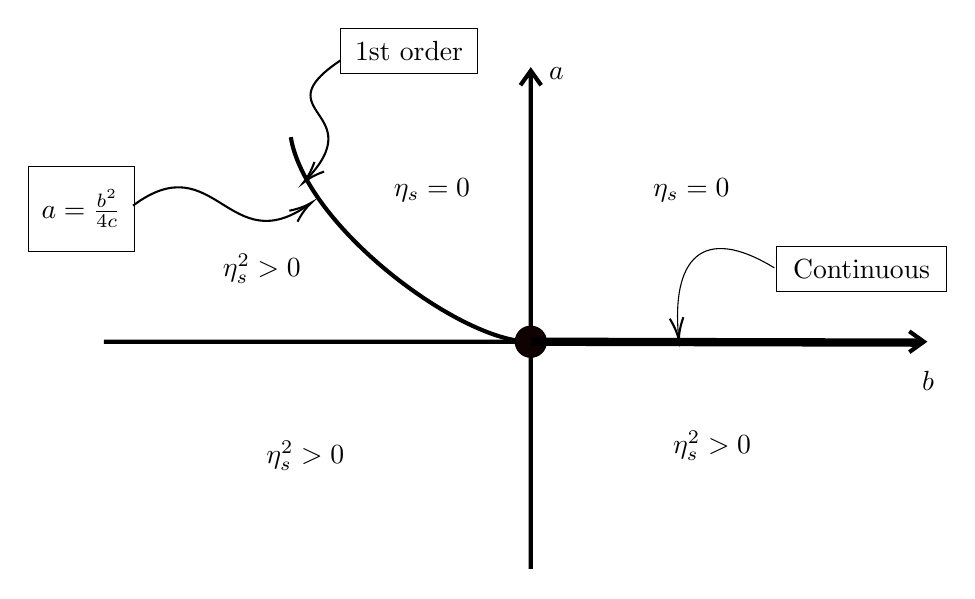
\begin{tikzpicture}[x=0.75pt,y=0.75pt,yscale=-1,xscale=1]
%uncomment if require: \path (0,300); %set diagram left start at 0, and has height of 300

%Shape: Axis 2D [id:dp49328105682435963] 
\draw [line width=1.5]  (135,160.04) -- (530,160.04)(340.64,29.47) -- (340.64,269.47) (523,155.04) -- (530,160.04) -- (523,165.04) (335.64,36.47) -- (340.64,29.47) -- (345.64,36.47)  ;
%Curve Lines [id:da5140430947735016] 
\draw [line width=1.5]    (225,61.47) .. controls (232,104.47) and (307,160.47) .. (340.64,160.04) ;


%Shape: Circle [id:dp6826221344791127] 
\draw  [fill={rgb, 255:red, 17; green, 2; blue, 2 }  ,fill opacity=1 ] (333.14,160.04) .. controls (333.14,155.9) and (336.49,152.54) .. (340.64,152.54) .. controls (344.78,152.54) and (348.14,155.9) .. (348.14,160.04) .. controls (348.14,164.19) and (344.78,167.54) .. (340.64,167.54) .. controls (336.49,167.54) and (333.14,164.19) .. (333.14,160.04) -- cycle ;
%Curve Lines [id:da752475905593098] 
\draw [line width=0.75]    (149,94.47) .. controls (188.6,64.77) and (194.88,121.84) .. (233.81,93.87) ;
\draw [shift={(235,93)}, rotate = 503.13] [color={rgb, 255:red, 0; green, 0; blue, 0 }  ][line width=0.75]    (10.93,-3.29) .. controls (6.95,-1.4) and (3.31,-0.3) .. (0,0) .. controls (3.31,0.3) and (6.95,1.4) .. (10.93,3.29)   ;

%Curve Lines [id:da1318138431983482] 
\draw [line width=0.75]    (249,24.47) .. controls (210.39,50.21) and (264.89,48.5) .. (232.02,82.43) ;
\draw [shift={(231,83.47)}, rotate = 315] [color={rgb, 255:red, 0; green, 0; blue, 0 }  ][line width=0.75]    (10.93,-3.29) .. controls (6.95,-1.4) and (3.31,-0.3) .. (0,0) .. controls (3.31,0.3) and (6.95,1.4) .. (10.93,3.29)   ;

%Curve Lines [id:da33663451695337276] 
\draw    (458,124.47) .. controls (422.54,102.8) and (408.42,120.91) .. (411.83,157.77) ;
\draw [shift={(412,159.47)}, rotate = 263.99] [color={rgb, 255:red, 0; green, 0; blue, 0 }  ][line width=0.75]    (10.93,-3.29) .. controls (6.95,-1.4) and (3.31,-0.3) .. (0,0) .. controls (3.31,0.3) and (6.95,1.4) .. (10.93,3.29)   ;

%Straight Lines [id:da5945398481130183] 
\draw [line width=3]    (527,160.47) -- (340.64,160.04) ;



% Text Node
\draw (532,179) node   {$b$};
% Text Node
\draw (353,31) node   {$a$};
% Text Node
\draw (293,87) node   {$\eta _{s} =0$};
% Text Node
\draw (418,87) node   {$\eta _{s} =0$};
% Text Node
\draw (428,210) node   {$\eta ^{2}_{s}  >0$};
% Text Node
\draw (232,215) node   {$\eta ^{2}_{s}  >0$};
% Text Node
\draw (211,125) node   {$\eta ^{2}_{s}  >0$};
% Text Node
\draw    (98.5,75.5) -- (149.5,75.5) -- (149.5,116.5) -- (98.5,116.5) -- cycle  ;
\draw (124,96) node   {$a=\frac{b^{2}}{4c}$};
% Text Node
\draw    (249,9) -- (315,9) -- (315,31) -- (249,31) -- cycle  ;
\draw (282,20) node  [align=left] {1st order};
% Text Node
\draw    (459,114) -- (541,114) -- (541,136) -- (459,136) -- cycle  ;
\draw (500,125) node  [align=left] {Continuous};


\end{tikzpicture}

When $\displaystyle a=0$ is approached with $\displaystyle b >0$, $\displaystyle \eta ^{2}_{s}$ is continuously reduced to zero. With $\displaystyle b< 0$, $\displaystyle \eta ^{2}_{s} =\frac{-b}{2c}$ on the line of $\displaystyle b^{2} =4ac$. Thus, the value of $\displaystyle \eta _{s}$ is changed abrubtly to $\displaystyle \eta _{s} =0$.



The origin in the plot above is a tricritical point because it can be reached by turing 3 variables, $\displaystyle t,\ p,$ and $\displaystyle h$ to 0 simultaneously.



(e) with $\displaystyle b=0$, we have $\displaystyle \mathcal{L}^{'} =a\eta +c\eta ^{5} -h=0$. At $\displaystyle h=0$ with $\displaystyle a< 0$, the solution is 

$\displaystyle \eta =( -a/c)^{1/4} =( -a_{1} t+a_{2} p/c)^{1/4} \Rightarrow \beta =\frac{1}{4}$

At $\displaystyle p=t=0$, the solution is $\displaystyle \eta =( h/c)^{1/5} \Rightarrow \delta =5$.

Thus susceptibility at $\displaystyle h=0$ is obtained by $\displaystyle \frac{\partial ^{2}\mathcal{L}}{\partial \eta ^{2}} |_{h=0}$:

$\displaystyle \left( a+5c\eta ^{4}\right)\frac{\partial \eta }{\partial h} -1=0\Rightarrow \frac{\partial \eta }{\partial h} =\frac{1}{a+5c\eta ^{4}} =\left\{\begin{matrix}
\frac{1}{a} & a >0\\
\frac{1}{-4a} & a< 0
\end{matrix}\right. \Rightarrow \gamma =\gamma ^{'} =1$



When $\displaystyle b=0$, we have $\displaystyle \mathcal{L} =\frac{1}{2} \eta ^{2}\left( a+\frac{1}{3} c\eta ^{4}\right)$. For $\displaystyle a >0,\eta =0\ and\ \mathcal{L} =0$. 

For $\displaystyle a< 0,\ \frac{\partial \mathcal{L}}{\partial \eta } =0,\ \eta =( -a/c)^{1/4} \ \ and\ \mathcal{L} =-\frac{1}{3} c\left( -\frac{a}{c}\right)^{3/2}$.

Because the heat capacity is the second derivative with respect to $\displaystyle t$, we have $\displaystyle \alpha =0,\ \alpha ^{'} =\frac{1}{2}$. Thus,

$\displaystyle \nu =\frac{2-\alpha }{d} =2/d$.

\section{Fluctuation and the Breakdown of Landau Theory}

\subsection{Breakdown of microscopic Landau theory}
In Landau theory, the term in the Hamiltonian of Ising model:
\begin{equation}
\sum_{i j} J_{i j} S_{i} S_{j}=\sum_{i} S_{i} \sum_{j} J_{i j}\left[\left\langle S_{j}\right\rangle+\left(S_{j}-\left\langle S_{j}\right\rangle\right)\right]
\end{equation}
by $\sum_{i j} S_{i} J_{i j}\left\langle S_{j}\right\rangle$. The fractional error implicit in this replacement can be quantified by the estimate:
\begin{equation}
E_{i j} \equiv \frac{\left|\left\langle S_{i} S_{j}\right\rangle-\left\langle S_{i}\right\rangle\left\langle S_{j}\right\rangle\right|}{\left\langle S_{i}\right\rangle\left\langle S_{j}\right\rangle}
\end{equation}
where all quantities are calculated using Landau theory for $T<T_{c}$. If we interested in estimate this error when $\left|\mathbf{r}_{\mathbf{i}}-\mathbf{r}_{\mathbf{j}}\right| \sim \boldsymbol{R},$ the range of the interaction. We have 
\begin{equation}
E_{R}=\frac{|G(R)|}{\eta_{s}^{2}}
\end{equation}
To calculate this, negligible fluctuation compared with the mean field is assumed. \bluep{if it should turn out that $\boldsymbol{E}_{\boldsymbol{R}} \geq 1$, then mean field theory would fail, because it would not be self-consistent, i.e. it would predict that a quantity is large when it was assumed initially to be small.}

\redp{Away from the critical point,} for $T \ll T_{c},$ the correlation length $\xi \sim R$, and 
\begin{equation}
\begin{aligned} \boldsymbol{E}_{\boldsymbol{R}} &=\boldsymbol{g} \times O(1) \sim \frac{k_{B} T}{\gamma} \xi^{2-d} \\ & \approx \frac{T}{T_{c}} \cdot \frac{\boldsymbol{a}^{d}}{R^{2}} \cdot R^{2-d} \approx\left(\frac{T}{T_{c}}\right)\left(\frac{\boldsymbol{a}}{R}\right)^{d} \end{aligned}
\end{equation}
Now $(R / a)^{d}$ is essentially the coordination number $z>1 ;$ hence, $E_{R}<1$
and mean field theory is self-consistent.

In summary, \redp{mean field theory works well when the co-ordination number is large.}

\redp{Near the critical point,}
\begin{equation}
E_{R} \sim \frac{1}{|t|^{2 \beta}}\left(\frac{a}{R}\right)^{d}
\end{equation}
which tends to \redp{infinity as the critical point is approached.}

\subsection{Breakdown of phenomenological Landau theory}
The criterion that $E_{LG}$ be small for the applicability of Landau theory is often referred to as the \textbf{Ginzburg criterion}\index{Ginzburg criterion}.
\begin{equation}
E_{L G}=\frac{\left|\int_{V} d^{d} \mathbf{r} G(\mathbf{r})\right|}{\int_{V} d^{d} \mathbf{r} \eta(\mathbf{r})^{2}}=\frac{k_{B}}{4 \Delta C \xi(1)^{d}} \frac{1}{|t|^{2-d / 2}}
\end{equation}
where $V$ is taken to be the correlation volume: $V=\xi(T)^{d}$. The condition that Landau theory be self-consistent, \textit{i.e.,}$E_{L G} \ll 1,$ requires that 
\begin{equation}
|t|^{(4-d) / 2} \gg \frac{k_{B}}{4 \Delta C \xi(1)^{d}} \equiv t_{L G}^{(4-d) / 2}
\end{equation}

From above, \redp{$\mathbf{d}>\mathbf{4} :$ As $t \rightarrow \mathbf{0},$ the Ginzburg criterion is always satisfied. $\mathbf{d}<\mathbf{4} :$ As $t \rightarrow \mathbf{0},$ the Ginzburg criterion is not satisfied.}

A useful way of stating the above conclusions is that for $d<4$, the quartic term proportional to $\eta^4$ in $\mathcal{L}$ becomes increasingly important as $t\rightarrow 0$, whilst the quartic term is negligible as $t\rightarrow 0$ for $d>4$.

In particular, whilst it is often (but not always) true that there is a dimensionality above which Landau theory is self-consistent, that dimension is \redp{not always d = 4}. This special dimension is called the \redp{upper critical dimension}\index{upper critical dimension} and
\begin{equation}
\frac{2 \beta+\gamma}{\nu} \equiv d_{c}
\end{equation}

\redp{The actual temperature $T_c$ at which the phase transition occurs must be lower than this temperature,} as can be seen by following argument: \tealp{In Landau theory, the long wavelength fluctuations are neglected, and the transition occurs at some $T_{c}^{0}$ where the short range fluctuations dominate the energy. Now imagine the same system at the same temperature as before, but including fluctuations of the order parameter i.e. the long wavelength fluctuations. Since there are more fluctuations, the entropy will be higher, and the system more disordered. At a given temperature, the real system is more disordered than as described by Landau theory. Consequently, the temperature at which the entropy begins to dominate the energy is lower than in Landau theory.}

\redp{The size of the critical region increases by lowering the dimensionality.}

\subsection{The Gaussian Approximation}
In this approximation, the fluctuations
turn out to be non-interacting i.e. independent random variables. This is why the Gaussian approximation is exactly soluble.

For a statistical mechanical system with one degree of freedom $q$ and Hamiltonian $H(q),$ the probability distribution for $q$ is:
\begin{equation}
P(q) \propto e^{-\beta H(q)} \approx e^{-\beta H\left(q_{0}\right)-\frac{1}{2}\left(q-\varphi_{0}\right)^{2} / \lambda^{2}}
\end{equation}
where we have performed a Taylor expansion about the maximum of $P(q)$:
\begin{equation}
H(q)=H\left(q_{0}\right)+\left.\frac{1}{2} \frac{\partial^{2} H}{\partial q^{2}}\right|_{q0}\left(q-q_{0}\right)^{2}
\end{equation}
and $\frac{1}{\lambda^{2}}=\beta \frac{\partial^{2} H}{\partial q^{2}}\left(q_{0}\right)$. Since $H(q_0)$ is just some constant, we can say that $(q-q_0)$--the fluctuation--is distributed normally. Hence:
\begin{equation}
\begin{aligned}\langle q\rangle &=\int_{-\infty}^{\infty} P(q) q d q=q_{0} \\\left\langle\left(q-q_{0}\right)^{2}\right\rangle &=\left\langle q^{2}\right\rangle- q_{0}^{2}=\left\langle q^{2}\right\rangle-\langle q\rangle^{2}=\lambda^{2} \end{aligned}
\end{equation}
\redp{The condition that the probability distribution be sharply peaked about its mean value is just the Ginzburg criterion}:
\begin{equation}
E_{G} \equiv \frac{\left\langle q^{2}\right\rangle-\langle q\rangle^{2}}{\langle q\rangle^{2}}=\frac{\lambda^{2}}{q_{0}^{2}} \ll 1
\end{equation}
The free energy is easily calculated in the Gaussian approximation:
\begin{equation}
\begin{array}{c}{e^{-F / k_{B} T}=\int_{-\infty}^{\infty} d q e^{-H(q) / k_{B} T}} \\ {=e^{-\beta H\left(q_{0}\right)} \sqrt{2 \pi \lambda^{2}}} \\ {F=H\left(q_{0}\right)-\frac{1}{2} k_{B} T \log \left(2 \pi \lambda^{2}\right)}\end{array}
\end{equation}

The extension of the above argument to \bluep{N degree of freedom} is straightforward. For $\mathbf{q}=\left(\boldsymbol{q}_{\mathbf{1}}, \boldsymbol{q}_{2}, \ldots, \boldsymbol{q}_{N}\right)$:
\begin{equation}
H(\mathbf{q})=H\left(\mathbf{q}_{0}\right)+\left.\frac{1}{2}\left(q_{\alpha}-q_{\alpha}^{0}\right) \frac{\partial^{2} H}{\partial q_{\alpha} \partial q_{\beta}}\right|_{\mathbf{q}=\mathbf{q}_{0}}\left(q_{\beta}-q_{\beta}^{0}\right)+\cdots
\end{equation}
The fluctuation matrix:
\begin{equation}
\left.M_{\alpha \beta} \equiv \frac{\partial^{2} H}{\partial q_{\alpha} \partial q_{\beta}}\right|_{q=q_{0}}
\end{equation}
can be diagonalized by finding its eigenvalues $\hat{\lambda}_{i}$ and eigenvectors $\mathbf{v}^{(i)}$:
\begin{equation}
\begin{array}{c}{M_{\alpha \beta} v_{\beta}^{(i)}=\hat{\lambda}_{i} v_{\alpha}^{(i)}} \\ {\frac{1}{\lambda_{i}^{2}} \equiv \beta \hat{\lambda}_{i}}\end{array}
\end{equation}
then
\begin{equation}
\beta H(\mathbf{q})=\beta H\left(\mathbf{q}_{0}\right)+\frac{1}{2} \sum_{i=1}^{N} q_{i}^{\prime 2} / \lambda_{i}^{2}
\end{equation}
where the $q_i^{\prime}$ are the components of the normal coordinates, i.e. the eigenvectors. The calculation of the free energy is:
\begin{equation}
\begin{aligned} e^{-\beta F} &=\int_{-\infty}^{\infty} \prod_{i=1}^{N} d q_{i} e^{-\beta H(\mathbf{q})} \\ & \simeq e^{-\beta H\left(\mathbf{q}_{0}\right)} \int_{-\infty}^{\infty} \prod_{i=1}^{N} d q_{i} e^{-\frac{1}{2} \beta\left(q_{\alpha}-q_{\alpha}^{0}\right) M_{\alpha \beta}\left(q_{\beta}-q_{\alpha}^{0}\right)}  \end{aligned}
\end{equation}
$=e^{-\beta H\left(\mathbf{q}_{0}\right)} \int \prod_{i=1}^{N} d q_{i}^{\prime} e^{-\frac{1}{2} \sum_{i=1}^{N} q_{i}^{\prime 2} / \lambda_{i}^{2}}$
$=e^{-\beta H\left(\mathbf{q}_{0}\right)} \prod_{i=1}^{N}\left[\int_{-\infty}^{\infty} d q_{i}^{\prime} e^{-\frac{1}{2} q_{i}^{\prime 2} / \lambda_{i}^{2}}\right]$

Performing the final integrations yields
\begin{equation}
F=H\left(\mathbf{q}_{0}\right)-\frac{1}{2} k_{B} T \sum_{i=1}^{N} \log \left(2 \pi \lambda_{i}^{2}\right)
\end{equation}
\subsubsection{Infinite Number of DOF}
We evaluate the functional integral:
\begin{equation}
e^{-\beta F}=\int D \eta e^{-\beta L\{\eta(\mathrm{r})\}}
\end{equation}
with
\begin{equation}
L=\int_{V} d^{d} r\left[\frac{1}{2} \gamma(\nabla \eta)^{2}+a t \eta^{2}+\frac{1}{2} b \eta^{4}-H \eta\right]+a_{0} V
\end{equation}
In the spirit of the Gaussian approximation, we shall:

\redp{(1)Find the uniform configuration which minimises $L .$ For $T>T_{c},$ this is $\eta=0,$ whereas for $T<T_{c},$ this is $\eta=\pm \sqrt{-a t / b} .$}

\redp{(2) Expand $L$ about the appropriate minimum to quadratic order in the fluctuation. Here, we will work above Tc, so we simply neglect the quartic terms in equation above.}

We begin by writing L in Fourier space, after dropping the quartic terms (define $\eta(r)=\frac{1}{V}\sum_k\eta_k e^{ik\cdot r}$):
\begin{equation}
\begin{aligned} L &=\int d^{d} \mathbf{r}\left[\frac{1}{2} \gamma(\nabla \eta)^{2}+a t \eta^{2}\right]+a_{0} V \\ &=\sum_{\mathbf{k} \mathbf{k}^{\prime}} \int \frac{d^{d} \mathbf{r}}{V^{2}}\left[\left(\frac{1}{2} \gamma\left(-\mathbf{k} \cdot \mathbf{k}^{\prime}\right)+a t\right) \eta_{\mathbf{k}} \eta_{\mathbf{k}^{\prime}}\right] e^{i\left(\mathbf{k}+\mathbf{k}^{\prime}\right) \cdot \mathbf{r}}+a_{0} V \end{aligned}
\end{equation}
\begin{equation}
=\frac{1}{V} \sum_{\mathbf{k}} \frac{1}{2}\left|\eta_{\mathbf{k}}\right|^{2}\left[\mathbf{2} a t+\gamma \boldsymbol{k}^{2}\right]+\boldsymbol{a}_{\mathbf{0}} V
\end{equation}

The free energy is given by
\begin{equation}
\begin{aligned} e^{-\beta F} &=\int_{-\infty}^{\infty} \prod_{\mathbf{k}}^{\prime} d \eta_{\mathbf{k}} e^{-\beta L} \\ &=\prod_{\mathbf{k}}^{\prime} \int_{-\infty}^{\infty} d \eta_{\mathbf{k}} e^{-\beta\left(2 a t+\gamma k^{2}\right)|\eta_k |^{2} / 2 V} \cdot e^{-\beta a_{0} V} \end{aligned}
\end{equation}
Writing $x \equiv \operatorname{Re} \eta_{\mathbf{k}}, y \equiv \operatorname{Im} \eta_{\mathbf{k}}$, each integral is of the form:
\begin{equation}
\int_{-\infty}^{\infty} d x d y e^{-A\left(x^{2}+y^{2}\right)}=\frac{\pi}{A}
\end{equation}
Taking account of the fact that $\eta(r)$ is real:
\begin{equation}
\begin{aligned} e^{-\beta F} &=\left(\prod_{\mathbf{k}} \frac{2 \pi V k_{B} T}{2 a t+\gamma k^{2}}\right) e^{-\beta a_{0} V} \\ &=\exp \left\{\frac{1}{2} \sum_{|\mathbf{k}|<\Lambda} \log \left[\frac{2 \pi V k_{B} T}{2 a t+\gamma k^{2}}\right]\right\} e^{-\beta a_{0} V} \end{aligned}
\end{equation}
where the $\Sigma_{k}$ in eqn. $(6.46)$ is over all $k$ -space, and so a factor of 1$/ 2$ has been inserted. Thus
\begin{equation}
F=a_{0} V-\frac{1}{2} k_{B} T \sum_{|\mathbf{k}|<\Lambda} \log \frac{2 \pi V k_{B} T}{2 a t+\gamma k^{2}}
\end{equation}
\subsubsection{Two-point Correlation Function Revisited}
We can calculate the two-point correlation function by using the \bluep{equipartition of energy}\index{equipartition of energy}. Thus,
\begin{equation}
\left\langle\left|\eta_{k}\right|^{2}\right\rangle \frac{2 a t+\gamma k^{2}}{V}=2 \times \frac{k_{B} T}{2}
\end{equation}
\bluep{The theorem of the equipartition of energy states that if a degree of freedom makes only a quadratic contribution to the Hamiltonian, then the average energy of the corresponding term in the Hamiltonian is $k_BT/2$.} Hence
\begin{equation}
\left\langle\left|\eta_{k}\right|^{2}\right\rangle=\frac{k_{B} T V}{2 a t+\gamma k^{2}}
\end{equation}
and 
\begin{equation}
\begin{aligned}\left\langle\left|\eta_{\mathbf{k}}\right|^{2}\right\rangle &=\int d^{d} \mathbf{x} d^{d} \mathbf{y} e^{i \mathbf{k} \cdot(\mathbf{y}-\mathbf{x})}\langle\eta(\mathbf{y}) \eta(\mathbf{x})\rangle \\ &= V \hat{G}(\mathbf{k}) \end{aligned}
\end{equation}
\begin{equation}
\hat{G}(\mathbf{k})=\frac{k_{B} T}{2 a t+\gamma k^{2}}=\frac{k_{B} T}{\gamma} \cdot \frac{1}{k^{2}+\xi_{>}^{-2}}
\end{equation}

\subsection{Solutions to Exercises}
6-1 (a)

For $\displaystyle T< T_{c}$, the minimum of Landau free energy is at $\displaystyle \eta _{s} =\sqrt{a/b| t|}$. Becuase $\displaystyle \nabla \eta _{s} =0$, we can expand Landau free energy as:

$\displaystyle  \begin{array}{l}
L=\int d^{d} r\left\{at\eta ^{2}_{s} +\frac{1}{2} b\eta ^{4}_{s}\right\} +a_{0} V+\int d^{d} r\left\{\frac{1}{2} \gamma \nabla \phi \cdot \nabla \phi +at\phi ^{2} +3b\eta ^{2}_{s} \phi ^{2}\right\}\\
=\left( a_{0} -\frac{a^{2}}{2b} t^{2}\right) V+\int d^{d} r\left\{\gamma \nabla \phi \cdot \nabla \phi +2a|t|\phi ^{2}\right\}
\end{array}$

Where the quartic term is neglected. Let $\displaystyle \phi \left(\vec{r}\right) =\frac{1}{V}\sum _{k} \eta _{k} e^{i\vec{k} \cdot \vec{r}}$, following the process in the book, we find:

$\displaystyle L=\left( a_{0} -\frac{a^{2}}{2b} t^{2}\right) V+\sum _{\vec{k}}\frac{1}{2}\left( \gamma k^{2} +4a|t|\right) |\eta _{\vec{k}} |^{2}$



(b) The partition function is now:

$\displaystyle Z=\int \mathcal{D} \phi e^{-\beta L} =e^{-\beta F}$

By following the equations on the book from (6.43) to (6.47), The free energy is:

$\displaystyle F=\left( a_{0} -\frac{a^{2}}{2b} t^{2}\right) -\frac{1}{2} k_{B} T\sum _{|\vec{k} |< \Lambda } log\frac{2\pi Vk_{B} T}{\gamma k^{2} +4a|t|}$

Because $\displaystyle \sum _{|\vec{k} |< \Lambda } =V\int _{|\vec{k} |< \Lambda }\frac{d^{d} k}{( 2\pi )^{d}}$ at the continuum limit, we find

$\displaystyle c_{-} =\frac{T_{c} k_{B} T_{c} V}{2V}\int _{|\vec{k} |< \Lambda }\frac{d^{d} k}{( 2\pi )^{d}}\frac{\left( -\frac{4a}{T_{c}}\right)^{2}}{\left( \gamma k^{2} +2a|t|^{2}\right)} =k_{B}\frac{16a^{2} \pi ^{d/2}}{\gamma ^{2}( 2\pi )^{d} \Gamma ( d/2)}\int ^{\Lambda }_{0} dk\frac{k^{d-1}}{\left( k^{2} +\xi ^{-2}\right)^{2}}$

where $\displaystyle \xi ^{2} =\frac{\gamma }{4a|t|}$. For $\displaystyle \Lambda \rightarrow \infty $, we have

$\displaystyle c_{-} =k_{B}\frac{16}{( 4\pi )^{d/2} \Gamma ( d/2)}\frac{a^{2}}{\gamma ^{2}}\int ^{\infty }_{0} dk\frac{k^{d-1}}{\left( k^{2} +\xi ^{-2}\right)^{2}} =k_{B}\frac{8\Gamma ( 2-d/2)}{( 4\pi )^{d/2}}\frac{a^{2}}{\gamma ^{2}} \xi ^{4-d}$

Thus, the most singular contribution to the integral as $t\rightarrow 0$ is proportional to $(4a|t|)^{d/2-2}$. 

From the book, we know that 

$\displaystyle c_{+} =k_{B}\frac{4}{( 4\pi )^{d/2} \Gamma ( d/2)}\frac{a^{2}}{\gamma ^{2}}\int ^{\infty }_{0} dk\frac{k^{d-1}}{\left( k^{2} +\xi ^{-2}\right)^{2}}$, where $\displaystyle \xi ^{2} =\frac{\gamma }{2at}$.

Now, the ratio becomes:

$\displaystyle \frac{c_{+}}{c_{-}} =\frac{1}{4} 2^{2-d/2} =2^{-d/2}$, and it is a constant for a certain dimensionality.

\section{Anomalous Dimensions}
\subsection{Dimensional analysis of Landau theory}
Now we can show that for $d>4$, perturbatively including the interaction of the fluctuations leads to no new singular behaviour as $t \rightarrow 0$. On the other hand, for $d<4$, this perturbation theory is divergent: the perturbing parameter grows unboundedly as $T\rightarrow T_c$.

First, we need to \tealp{identify the single parameter in which a systematic expansion can be attempted.} We start with:
\begin{equation}
\begin{array}{c}{Z=\int D \eta e^{-\beta L}} \\ {L=\int d^{d} \mathbf{r}\left\{\frac{1}{2} \gamma(\nabla \eta)^{2}+a t \eta^{2}+\frac{1}{2} b \eta^{4}-H \eta\right\}}\end{array}
\end{equation}
rescale $\eta$ as:
\begin{equation}
\phi \equiv(\beta \gamma)^{1 / 2} \eta ; \quad \frac{r_{0}}{2} \equiv \frac{a t}{\gamma} \equiv \frac{1}{2} \overline{a} t ; \quad \frac{u_{0}}{4} \equiv \frac{1}{2} \frac{b}{\beta \gamma^{2}}
\end{equation}
With H=0, we have
\begin{equation}
H_{\mathrm{eff}}\{\phi\} \equiv L \beta=\int d^{d} \mathbf{r}\left[\frac{1}{2}(\nabla \phi)^{2}+\frac{1}{2} r_{0} \phi^{2}+\frac{1}{4} u_{0} \phi^{4}\right]
\end{equation}

\tealp{Now we identify the dimensions of the various quantities:}
\begin{equation}
\begin{array}{c}{\left[\int d^{d} \mathbf{r}(\nabla \phi)^{2}\right]=1 \Longrightarrow L^{d} \cdot L^{-2}[\phi]^{2}=1} \\ {[\phi]=L^{1-d / 2}}\end{array}
\end{equation}
\begin{equation}
\begin{array}{c}{\left[\int d^{d} \mathbf{r}_{0} \phi^{2}\right]=\left[\int d^{d} \mathbf{r} u_{0} \phi^{4}\right]=1} \\ {\left[r_{0}\right]=L^{-2} ; \quad\left[u_{0}\right]=L^{d-4}}\end{array}
\end{equation}

\tealp{Then, we rewrite $H_{eff}$ in terms of dimensionless variables:$\varphi, \overline{u}_{0},$ which are $\phi$ and $u_0$ scaled by the appropriate powers of $r_0$}. Since $\xi\sim t^{-1/2}$ and $r_0\propto (T-T_c)$, we know that within the Gaussian approximation (order parameter contribute to L up to quadratic term): $r_{0} \propto 1 / \xi(T)^{2} .$ Using $r_{0}^{-1 / 2}$ as the length scale is equivalent to measuring lengths in units of the correlation length $\xi(T)$. To do Gaussian functional integral, we define the following dimensionless variables:
\begin{equation}
\varphi \equiv \frac{\phi}{L^{1-d / 2}} ; \quad \mathbf{x} \equiv \frac{\mathbf{r}}{L} ; \quad \overline{u}_{0} \equiv \frac{u_{0}}{L^{d-4}} ; \quad L \equiv r_{0}^{-1 / 2}
\end{equation}
Now the partition function becomes:
\begin{equation}
\begin{aligned} Z\left(\overline{u}_{0}\right) &=\int D \varphi \exp \left[-H_{0}\{\varphi\}-H_{\text {int }}\{\varphi\}\right] \\ H_{0} &=\int d^{d} \mathbf{x}\left\{\frac{1}{2}(\nabla \varphi)^{2}+\frac{1}{2} \varphi^{2}\right\} \\ H_{\text {int }} &=\int d^{d} \mathbf{x}\left\{\frac{1}{4} \overline{u}_{0} \varphi^{4}\right\} \end{aligned}
\end{equation}
If $H_{\mathrm{int}}=0,$ the integral is just the Gaussian approximation.\tealp{The partition function has, however, a contribution from the interactions, $H_{int}$.} We might imagine that if $\bar u_0 \ll 1$, then we could use \bluep{perturbation theory}\index{perturbation ! theory}:
\begin{equation}
\begin{aligned} Z &=\int D \varphi e^{-H_{0}} e^{-H_{\mathrm{int}}} \\ &=\int D \varphi e^{-H_{0}}\left(1-H_{\mathrm{int}}+\frac{1}{2 !}\left(H_{\mathrm{int}}\right)^{2}-\cdots\right) \end{aligned}
\end{equation}
\redp{The partition function depends on one dimensionless parameter $\bar u_0$}; this is the \redp{perturbation parameter}\index{perturbation!parameter}:
\begin{equation}
\overline{u}_{0}=u_{0} r_{0}^{(d-4) / 2}=u_{0} \overline{a}^{(d-4 / 2)} t^{(d-4) / 2}
\label{u_0_bar}
\end{equation}
\tealp{As $t \rightarrow 0,$ for $d<4, \overline{u}_{0} \rightarrow \infty$ and perturbation theory becomes meaningless. On the other hand, for $d>4, \pi_{0} \rightarrow 0$ as $t \rightarrow 0,$ and mean field becomes increasingly accurate as $T \rightarrow T_{c}^{+}$.}

Now, it is reasonable that \bluep{perturbation theory will break down when the expansion parameter is of order unity.} Thus, the critical region is the range of $t$ for which $\overline{u}_{0} \geq O(1)$. From the equation\ref{u_0_bar} we have:
\begin{equation}
t^{(4-d) / 2} \geq \frac{b}{a^{2}} \frac{1}{\xi(1)^{d}}
\end{equation}
Because we only show that each term in the perturbation theory are divergent as $t\rightarrow 0$, \tealp{this does not mean necessarily that the actual perturbation series is divergent, when summed.}\bluep{Resummations of apparently divergent series form the basis for the most accurate estimates of critical exponents.}

For $d>4$, it's also not true that perturbation theory necessarily converges.(smallness of expansion parameter$\neq$convergence) What happens to $Z$ if we make the transformation $\overline{u}_{0} \rightarrow-\overline{u}_{0} ?$
\begin{equation}
Z\left(-\overline{u}_{0}\right)=\int D \varphi e^{-\int d^{d} x\left[\frac{1}{2}(\nabla \varphi)^{2}+\frac{1}{2} \varphi^{2}\right]+\int d^{d} x \overline{x}_{0} \varphi^{4}}
\end{equation}
which is divergent due to the sign of the quartic term. On the other hand
\begin{equation}
Z\left(\overline{u}_{0}\right)=\int D \varphi e^{-\int d^{d} x\left[\frac{1}{2}(\nabla \phi)^{2}+\frac{1}{2} \varphi^{2}\right]-\int d^{4} x \overline{v}_{0} \varphi^{4}}
\end{equation}
is convergent. Thus $\bar u_0$ is not a regular point.
\subsection{Dimensional Analysis and Critical Exponents}
Now we show that \tealp{it is impossible for the critical exponents to have values different from those predicted by Landau theory}.

First, we perform dimensional analysis for the two-point correlation function:
\begin{equation}
G\left(\mathbf{r}-\mathbf{r}^{\prime}\right) \equiv\left\langle\phi(\mathbf{r}) \phi\left(\mathbf{r}^{\prime}\right)\right\rangle=\frac{\int D \phi e^{-H_{\mathrm{eff}}\{\phi\}} \phi(\mathbf{r}) \phi\left(\mathbf{r}^{\prime}\right)}{\int D \phi e^{-H_{\mathrm{eff}}\{\phi\}}}
\end{equation}
Thus, 
\begin{equation}
\begin{array}{c}{\left[G\left(\mathbf{r}-\mathbf{r}^{\prime}\right)\right]=[\phi]^{2}=L^{2-d}} \\ {\hat{G}(\mathbf{k})=\frac{1}{V} \int d^{d} \mathbf{x} d^{d} \mathbf{y} e^{-i \mathbf{k} \cdot(x-y)} G(\mathbf{x}-\mathbf{y})}\end{array}
\end{equation}
Because $\langle|\eta|^2\rangle=V\hat G(\textbf{k})$, we have
\begin{equation}
[\hat{G}(\mathbf{k})]=L^{-d} L^{2 d} \cdot L^{2-d}=L^{2}
\end{equation}
if we make a change of the units of length by a factor of $\epsilon$ from $L$ to $L^{\prime} \equiv \epsilon L,$ then $\hat{G}$ should transform according to the rule that $\hat{G}^{\prime} L^{\prime 2}=$ $\hat{G} L^{2}$, which implies that 
\begin{equation}
\label{DA_eta}
\hat{G}^{\prime}\left(\mathbf{k}^{\prime}\right)=\epsilon^{-2} \hat{G}(\mathbf{k})
\end{equation}
We are using the convention that a physical quantity $Q_p$ represented by the symbol $Q_p=Q[Q]$. The symbol $[Q]$ designates the units that must be appended to $Q$. Under a change of unit, Q changes, whilst $Q_p$ is invariant.

With $\mathbf{k}^{\prime}=\epsilon \mathbf{k}$, this result must always be true: it follows simply from the definition of the two point function.

At $T_c$, in defining the critical exponent $\eta$, we have asserted that at long wavelengths $(\boldsymbol{k} \rightarrow \mathbf{0})$:
\begin{equation}
\label{critical_eta}
\hat{G}\left(\mathbf{k}, T_{c}\right) \sim k^{-2+\eta}
\end{equation}
Under a change of length scale
\begin{equation}
\hat{G}^{\prime}\left(\mathbf{k}^{\prime}\right) \sim \epsilon^{-2+\eta} \hat{G}(\mathbf{k})
\end{equation}
\bluep{Unless $\eta=0$, the value given by Landau theory, this clearly disagrees with our preceding general dimensional considerations.}

\redp{This is, the central mystery of critical phenomena: any value for the critical exponents other than that given by Landau theory seems to violate dimensional analysis.}

How could the equation \ref{DA_eta} and \ref{critical_eta} both be correct?\redp{ There must be another length scale which comes into the dimensional analysis, apart from the correlation length.} The only other length scale
in the problem is the \bluep{microscopic length scale - the lattice spacing $a$, or the short distance cut-off given by $\Lambda^{-1}$}. And they must be included in the dimensional analysis.

For the correlation length, if we redo the dimensional analysis taking into account the microscopic length scale $a$, we have the relations:
\begin{equation}
[\xi]=L ; \quad[a]=L ; \quad\left[r_{0}\right]=L^{-2}
\end{equation}
As $r_0\propto t$, we conclude that
\begin{equation}
\xi=r_{0}^{-1 / 2} f\left(r_{0} a^{2}\right)
\end{equation}
When $t \rightarrow 0,$ the argument of $f$ tends to zero. If it so happens that
\begin{equation}
f(x) \sim x^{\theta}, \quad \text { as } x \rightarrow 0
\end{equation}
for some $\theta$ to be determined, then as $t\rightarrow 0$,
\begin{equation}
\xi \sim t^{-1 / 2+\theta} a^{2 \theta}
\end{equation}
Thus the critical exponent governing the divergence of the correlation length is
\begin{equation}
\nu=\frac{1}{2}-\theta
\end{equation}
The difference between this result and that of Landau theory is the so-called \textbf{\bluep{anomalous dimension $\theta$}}\index{anomalous dimension}.

\tealp{How does the microscopic length scale affect correlations at macroscopic distances?} Suppose that we are
interested in some quantity $F$ that depends in principle on $a$ and $\xi$. Then, it is only legitimate to replace $a/\xi$ by 0 in the function $F(A/\xi)$ if $F(x)$ is not singular in the limit $x\rightarrow 0$. There are three possibilities for this limit:
(1) $F(x) \rightarrow 0$ as $x \rightarrow 0 .$

(2) $F(x) \sim x^{-\sigma} \Phi(x)$ as $x \rightarrow 0,$ with $\sigma>0$ and $\Phi(x)$ regular in the limit that $x \rightarrow 0 .$

(3) None of the above.

\tealp{From the preceding discussion, it follows that critical phenomena are in case (2) above.}

\subsection{Renormalization and Anomalous Dimensions}
Now, we briefly discuss the notion of \textbf{renormalization} in \textbf{field theory}\index{field theory}. \redp{Field theory is a term used to denote any model system described by a functional integral}.

In quantum field theory, however, the time variable t is first analytically continued from the real axis to the imaginary axis $\tau ( \tau = -it)$, in order that the functional integral be convergent. Such field theories are sometimes known as Euclidean, because after the analytic continuation has been performed, the metric of space-time, with interval s given by $ds^2 = dr^2 + dr^2$ , describes a flat (Euclidean) manifold rather than the original curved manifold of Minkowski space, in which $ds^2 = dr^2 - dt^2$.

In quantum field theory, however, where we have assumed that there is no microscopic physics to contribute a cut-off $\Lambda$, we must try to make sense of the divergence that we have found. The procedure that is followed - renormalisation - consists of a sequence of steps. First, an artificial cut-off $\Lambda$ is introduced into the theory; this is sometimes known as regularisation. Next, the desired calculation is performed, and is perfectly finite. Finally, the limit $\Lambda\rightarrow \infty$ is taken, absorbing the resultant infinities into a redefinition of the parameters in $H_{eff}$, such as $r_0$ and $u_0$.

\redp{The essential point is that the renormalisation
procedure introduces a new length scale into the problem.}

\subsection{Solution to Exercises}
(a) A stationary configuration $\varphi_s$ must minimize $L$, and is constant. Thus, the stationary equation is:

$r_{0} \phi+\frac{1}{(n-1) !} u_{n} \phi^{n-1}-0$

If $r_0<0$, we have a nonegative solution:

$\phi_{s}=\left(\frac{(n-p) !\left|r_{0}\right|}{u_{n}}\right)^{\frac{1}{n-2}}$

The correlation length can be obtained by setting $\phi(\vec{x})=\phi_{s}+\psi(\vec{x})$ and expanding $L$ to second order in $\psi$:

$\begin{aligned} L=& \int d^{d} x\left(\frac{1}{2} r_{0} \phi_{s}^{2}+\frac{1}{n !} u_{n} \phi_{s}^{n}\right) \\ &+\int d^{d} x\left(\frac{1}{2} \nabla \psi \cdot \nabla \psi+\frac{1}{2} r_{0} \psi^{2}+\frac{1}{2(n-2)!} u_{n} \phi_{s}^{n-2} \psi^{2}\right) \end{aligned}$

$\begin{aligned}=& V\left(\frac{1}{2} r_{0} t_{s}^{2}-\frac{r_{0}}{n} k_{s}^{2}\right) \\ &+\int d^{d} x\left(\frac{1}{2} \nabla \psi \cdot \nabla \psi+\frac{1}{2} \xi^{-2} \psi^{2}\right) \end{aligned}$

The correlation length is now given by:

$\begin{aligned} \xi^{-2} &=r_{0}+\frac{1}{(n-2) !} u_{n} \phi_{s}^{n-2} \\ &=r_{0}+(n-1)\left|r_{0}\right| \\ &=(n-2)\left|r_{0}\right| \end{aligned}$

The Ginzburg criterion is

$\int d^{2} r G(r)\ll \int d^{d} r\left\langle\phi^{2}\right\rangle$

With $\gamma=1$, we know $2 a t=\xi^{-2}$. Now the integral of $G(r)$ is:$\int d^{d} r G(r)=k T \xi^{2}$. If we further set $\left\langle \phi^{2}\right\rangle-\phi_{s}^{2}$, we have:

$\int d^{d} r\left\langle\phi^{2}\right\rangle \approx \xi^{d} \cdot \phi_{s}^{2}$

Now the criterion is reduced to:$k T_{c} \xi^{2}<\varepsilon_{d} \cdot \phi_{s}^{2}$. Expand $\xi$ and $\phi_s$, we obtain:

$k T_{c} \cdot \frac{1}{(n-2)\left|r_{0}\right|}\ll\left(\frac{1}{(n-2)\left|r_{0}\right|}\right)^{d / 2}\left(\frac{(n-1) !(r_0)}{u_{n}}\right)^{\frac{2}{n-2}}$

Thus, $\left|r_{0}\right|^{\frac{d-2}{2}-\frac{2}{n-2}}<<\frac{1}{k T_{c}\left(u_{n}\right)^{2 /(n-2)}}$. Now, the criterion is satisfied as $t\rightarrow 0$ (i.e., $r_0=at$) only if $\frac{d-2}{2}-\frac{2}{n-2}>0$, which gives the critical dimension $d=2+\frac{4}{n-2}=\frac{2n}{n-2}$.

\section{Scaling Laws}
Are critical exponents independent? No.

\textbf{Rushbrooke scaling law}, an example of thermodynamic scaling laws:
\begin{equation}
\begin{array}{c}{\alpha+2 \beta+\gamma=2} \\ {\beta \gamma=\beta+\gamma}\end{array}
\end{equation}

There are also scaling laws for the correlation function exponents, \textbf{Josephson scaling law}:
\begin{equation}
2-\alpha=\nu d
\end{equation}
where the law involves the dimensionality directly, and is an example of a \textbf{hyperscaling law}\index{hyperscaling law}.

\subsection{Small Time-Dependent Fluctuations}
In equilibrium, the spatial configuration of the order parameter is given by
\begin{equation}
\frac{\delta L}{\delta \eta(\mathbf{r})}=0
\end{equation}
\begin{equation}
L=\int d^{d} \mathbf{r}\left\{\frac{1}{2} \gamma(\nabla \eta)^{2}+\tilde{a} \eta^{2}+\frac{1}{2} b \eta^{4}-H \eta\right\}
\end{equation}
If the system is slightly out of equilibrium, it is not unnatural to guess that \bluep{the rate at which the system relaxes back to equilibrium is proportional to the deviation from equilibrium.} This assumption of linear response is purely phenomenological, and leads to the following equation for the rate of change of the order parameter:
\begin{equation}
\frac{\partial \eta(\mathbf{r})}{\partial t}=-\Gamma \frac{\boldsymbol{\delta} L}{\delta \boldsymbol{\eta}(\mathbf{r})}
\end{equation}
where $\Gamma$ is a phenomenological parameter, which we will assume to be independent of $\eta$, and weakly temperature dependent (i.e. it has no singular temperature dependence).

This equation (known as the \textbf{time-dependent Ginzburg-Landau equation} in the theory of superconductivity) cannot possibly be a correct description of the approach to the equilibrium state, because the equilibrium state is actually a global minimum of L. \bluep{The Equation above will cause the order parameter to evolve towards local minima, but not necessarily the global minimum.}

To ensure that the system approaches the global
minimum, we must remember that actually the order parameter dynamics is not purely relaxational, but may exhibit fluctuations, arising from the microscopic degrees of freedom. These "\bluep{thermal fluctuations}" will sometimes cause the order parameter to \bluep{move further away from equilibrium
during its time evolution, and thus prevent the system from becoming trapped in any metastable minima of L that may be present.} This state of affairs may be modelled by introducing a noise term $\xi$ to give:
\begin{equation}
\frac{\partial \eta(\mathbf{r})}{\partial t}=-\Gamma \frac{\delta L}{\delta \eta(\mathbf{r})}+\zeta(\mathbf{r}, t)
\end{equation}
where the noise is assumed to be a Gaussian random function, with a probability distribution:
\begin{equation}
P_{\zeta}(\{\zeta(\mathbf{r}, t)\}) \propto \exp \left[-\frac{1}{2 D} \int d t d^{d} \mathbf{r} \zeta(\mathbf{r}, t)^{2}\right]
\end{equation}
and the variance of the distribution being D:
\begin{equation}
\langle\zeta(\mathbf{r}, t)\rangle_{\zeta}=0 ; \quad\left\langle\zeta(\mathbf{r}, t) \zeta\left(\mathbf{r}^{\prime}, t^{\prime}\right)\right\rangle_{\zeta}=D \delta\left(\mathbf{r}-\mathbf{r}^{\prime}\right) \delta\left(t-t^{\prime}\right)
\end{equation}
The notation $\langle\cdots\rangle_{\xi}$ denotes averaging with respect to the probability dis-
tribution $P_{\xi} .$ In order that the stochastic differential equation above, usually known as the Langevin equation\index{Langevin equation}, leads to the correct equilibrium probability distribution $P_{\eta}^e$ for $\eta$, the amplitude of the noise must be related to the temperature of the system.

The probability of finding the order parameter in the configuration $\eta(\mathbf{r})$ is a function of time, and is given by:
\begin{equation}
P_{\eta}(\{\eta(\mathbf{r})\}, t)=\langle\delta[\eta(\mathbf{r})-\overline{\eta}(\mathbf{r}, t,\{\zeta\})]\rangle_{\zeta}
\end{equation}
where $\overline{\eta}(\mathbf{r}, t,\{\zeta\})$ is a solution of the Langevin equation. The time evolution of $P_{\eta}$ may be found by differentiating the equation above, giving \textbf{Fokker-Plank equation}\index{Fokker-Plank equation}:
\begin{equation}
\partial_{t} P_{\eta}(\{\eta(\mathbf{r})\}, t)=\int d^{d} \mathbf{r}^{\prime} \frac{\delta}{\delta \eta\left(\mathbf{r}^{\prime}\right)}\left[\Gamma \frac{\delta L}{\delta \eta\left(\mathbf{r}^{\prime}\right)} P_{\eta}+\frac{D}{2} \frac{\delta P_{\eta}}{\delta \eta\left(\mathbf{r}^{\prime}\right)}\right]
\end{equation}
As $t \rightarrow \infty,$ the solution to the Fokker-Planck equation approaches the equalibrium solution
\begin{equation}
P_{\eta}^{\mathrm{e}}\{\eta(\mathbf{r})\} \propto \exp \left(-\frac{2 \Gamma L\{\eta(\mathbf{r})\}}{D}\right)
\end{equation}
\bluep{which should be the Boltzmann distribution}. For this to be the case, the strength of the fluctuations D must be related to the temperature T and the strength of the dissipation $\Gamma$ by:
\begin{equation}
D=2 \Gamma k_{B} T
\end{equation}
An example of the \textbf{fluctuation-dissipation theorem}\index{fluctuation-dissipation theorem}.

\printindex
\end{document}
